\documentclass{article}

\PassOptionsToPackage{numbers,sort&compress}{natbib}
\usepackage[preprint]{neurips_2026}

% =====================================================================
% Packages
% =====================================================================
\usepackage[utf8]{inputenc}
\usepackage[T1]{fontenc}
\usepackage{microtype}
\usepackage{amsmath,amssymb,amsthm,mathtools}
\usepackage{aliascnt}
\usepackage[shortlabels]{enumitem}
\usepackage{booktabs}
\usepackage{graphicx}
\usepackage{xcolor}
\usepackage{array}
\usepackage{tabularx}
\usepackage{multirow}
\usepackage{caption}
\usepackage{bm}
\usepackage[colorlinks=true,linkcolor=blue,citecolor=blue,urlcolor=blue]{hyperref}
\usepackage[capitalize,noabbrev,nameinlink]{cleveref}

% =====================================================================
% Theorem environments
% =====================================================================
\newtheorem{theorem}{Theorem}[section]
\newaliascnt{proposition}{theorem}
\newtheorem{proposition}[proposition]{Proposition}
\aliascntresetthe{proposition}
\newaliascnt{lemma}{theorem}
\newtheorem{lemma}[lemma]{Lemma}
\aliascntresetthe{lemma}
\newaliascnt{corollary}{theorem}
\newtheorem{corollary}[corollary]{Corollary}
\aliascntresetthe{corollary}
\newaliascnt{definition}{theorem}
\newtheorem{definition}[definition]{Definition}
\aliascntresetthe{definition}
\theoremstyle{remark}
\newaliascnt{remark}{theorem}
\newtheorem{remark}[remark]{Remark}
\aliascntresetthe{remark}
\newaliascnt{example}{theorem}
\newtheorem{example}[example]{Example}
\aliascntresetthe{example}

% Proper names for cleveref
\crefname{theorem}{theorem}{theorems}
\Crefname{theorem}{Theorem}{Theorems}
\crefname{proposition}{proposition}{propositions}
\Crefname{proposition}{Proposition}{Propositions}
\crefname{lemma}{lemma}{lemmas}
\Crefname{lemma}{Lemma}{Lemmas}
\crefname{corollary}{corollary}{corollaries}
\Crefname{corollary}{Corollary}{Corollaries}
\crefname{definition}{definition}{definitions}
\Crefname{definition}{Definition}{Definitions}
\crefname{remark}{remark}{remarks}
\Crefname{remark}{Remark}{Remarks}
\crefname{example}{example}{examples}
\Crefname{example}{Example}{Examples}

% =====================================================================
% Macros
% =====================================================================
\DeclareMathOperator*{\argmax}{arg\,max}
\DeclareMathOperator*{\argmin}{arg\,min}
\DeclareMathOperator{\sigmoid}{sigmoid}
\DeclareMathOperator{\Bern}{Bern}
\DeclareMathOperator{\Var}{Var}
\newcommand{\R}{\mathbb{R}}
\newcommand{\E}{\mathbb{E}}
\newcommand{\Prob}{\mathbb{P}}
\newcommand{\KL}{\mathrm{KL}}
\newcommand{\Hbin}{H_{\mathrm{bin}}}
\newcommand{\defeq}{\coloneqq}
\newcommand{\cS}{\mathcal{S}}
\newcommand{\cA}{\mathcal{A}}
\newcommand{\cT}{\mathcal{T}}
\newcommand{\cB}{\mathcal{B}}
\newcommand{\cF}{\mathcal{F}}
\newcommand{\cK}{\mathcal{K}}
\newcommand{\hbg}{h_{\beta,\gamma}}
\newcommand{\fbg}{f_{\beta,\gamma}}
\newcommand{\gbg}{g_{\beta,\gamma}}
\newcommand{\pprior}{p_0}
\newcommand{\KLbin}[2]{\KL\!\left(\Bern(#1)\,\middle\|\,\Bern(#2)\right)}
\newcommand{\Lip}{\mathrm{Lip}}
\newcommand{\bgL}[1]{L_{\beta,\gamma}(#1)}
\DeclareMathOperator{\PL}{PL}
\DeclareMathOperator{\clip}{clip}
\newcommand{\safe}{\mathrm{safe}}
\newcommand{\Ksafe}{\widehat{\mathcal K}}
\newcommand{\betacap}{\overline\beta}
\newcommand{\Bhat}{\widehat B}

% =====================================================================
\title{Selective Temporal Credit Assignment via Safe Weighted Log-Sum-Exp Bellman Operators}
\author{Pawel Polak}
\date{}

\begin{document}
\maketitle

\begin{abstract}
Classical discounted dynamic programming propagates value through a uniform temporal filter: every Bellman backup applies the same continuation coefficient $\gamma$, regardless of whether the informative signal is a rare opportunity, a regime shift, or a catastrophic warning. We develop a variational alternative based on weighted log-sum-exp Bellman operators, in which a KL-regularized temporal allocation variable chooses how much Bellman mass to assign to immediate reward and how much to assign to continuation. The resulting recursive utility is time-consistent, strictly richer than classical discounted dynamic programming, and recovers the classical Bellman target exactly at $\beta=0$.

The adaptive continuation coefficient is state- and advantage-dependent. We identify a precise strict-improvement regime over classical dynamic programming: whenever the signed advantage $\beta(r-V)$ is positive with a uniform margin, the adaptive continuation coefficient is strictly below $\gamma$ and the Bellman operator is locally more contractive than the classical operator. This mechanism is particularly relevant to sparse delayed rewards, nonstationary regime shifts, and tail-dominated control, where informative signals should propagate faster than under a fixed discount. Because the raw operator can also become expansive, we introduce a calibrated safe family that clips a deterministic stagewise temperature schedule against stagewise certification levels.

For the calibrated safe family we prove Bellman expectation and optimality equations, exact temporal comparator theorems, stagewise envelope bounds, exact backward induction, policy improvement and finite policy iteration, value iteration, a convex program for the optimistic regime, modified policy iteration, projected TD(0), Q-learning, expected-SARSA, and asynchronous convergence. We also show that the temporal allocation step admits exact post-transition Monte Carlo estimation and differentiable Binary Concrete / Gumbel-Softmax surrogates. The overall picture is that classical dynamic programming diffuses information uniformly over time, whereas weighted-LSE Bellman operators selectively amplify the informative parts of trajectories while remaining certifiably safe on the deployed domain.
\end{abstract}

% =====================================================================
\section{Introduction}
\label{sec:intro}
% =====================================================================

Classical discounted dynamic programming propagates value through a uniform temporal filter. Each Bellman backup mixes current reward and continuation with the same coefficient $\gamma$, and each trajectory contributes through the same additive averaging rule. This uniformity is mathematically elegant, but it is also structurally diffuse: rare high-payoff events, regime changes, sparse delayed rewards, and catastrophic losses are all propagated backward through the same inertial discount mechanism. In many decision problems the informative part of the trajectory is not uniform in time. The right Bellman update should amplify the informative portions of a trajectory and suppress the uninformative ones.

This paper develops a variational dynamic-programming framework that does exactly that. Our Bellman target is a weighted log-sum-exp operator with a KL-regularized temporal allocation variable $\rho_t$. At each stage the operator chooses how much Bellman mass to allocate to the immediate reward and how much to allocate to continuation. The resulting recursion remains time-consistent because it is defined recursively on the time-augmented horizon, and the allocation is exact rather than heuristic: \Cref{thm:recursive-decomposition} shows that the Bellman target is precisely the optimum of a binary temporal-allocation problem around the classical prior $p_0=1/(1+\gamma)$.

The main mechanism is the adaptive continuation coefficient
\[
d_{\beta,\gamma}(r,V) = \partial_V g_{\beta,\gamma}(r,V) = (1+\gamma)(1-\rho^*(r,V)).
\]
Classical dynamic programming uses the same continuation coefficient $\gamma$ everywhere. Our operator adapts it to the signed Bellman advantage. \Cref{prop:effective-discount} shows that $d_{\beta,\gamma}(r,V)\le \gamma$ exactly when $\beta(r-V)\ge 0$, with strict inequality unless $\beta=0$ or $r=V$. Hence the continuation term automatically shrinks on the regions of the state space where the sign of the advantage is aligned with the chosen risk bias. \Cref{thm:aligned-contraction} then identifies a precise strict-improvement regime: if $\beta(r-V)$ is uniformly positive by a margin $\eta$, the weighted Bellman operator is locally more contractive than the classical $\gamma$-Bellman operator.

This viewpoint touches several recent literatures, but on a different axis. Recursive OCE MDPs already study broad dynamic risk measures over cumulative return; our paper instead isolates a single Bellman-local operator family with a closed-form Bernoulli/KL temporal allocator and an explicit comparison to the classical continuation coefficient \citep{xu2023recursiveoce}. A recent reductions approach pushes that OCE program further by mapping risk-sensitive control to an augmented risk-neutral MDP; we do not reduce to an augmented classical problem, because the modified Bellman backup itself is the object of study here \citep{wang2025oce}. Near-minimax CVaR reinforcement learning optimizes a tail functional of cumulative return, whereas our operator does not target a quantile or coherent tail constraint at all \citep{wang2023near}. Risk-sensitive distributional reinforcement learning learns return laws under static risk measures; our theory stays scalar and asks how a deterministic nonlinear backup reallocates mass between reward and continuation \citep{chen2024distrl}. Risk-sensitive offline reinforcement learning is also adjacent, but its selectivity is about dataset support and pessimism under static data, whereas ours is temporal and can be used in either online or offline settings \citep{zhang2024riskoffline}. Reward shaping changes the reward signal itself; our method leaves the environment reward unchanged and changes only the Bellman operator \citep{ma2024assistant}. Sequence compression changes the temporal representation or abstraction level; our method keeps the representation fixed and changes only how each backup mixes reward and continuation \citep{ramesh2024chunked}. Pausing Policy Learning tackles drift by scheduling when policy updates occur; our operator can be inserted even when the update schedule is held fixed \citep{lee2024pausing}. COREP tackles drift through learned causal-origin state representations; we do not learn a representation or infer a change source \citep{zhang2024corep}. LCPO assumes observed exogenous contexts and constrains policy changes across contexts; our theory does not assume context labels and instead changes the backup map itself \citep{hamadanian2025lcpo}. Discount regularization shortens the horizon uniformly and can help or hurt depending on data coverage; our continuation coefficient is state- and advantage-dependent and recovers the classical backup exactly at $\beta=0$ \citep{rathnam2024discount}. Selective Bellman trust regularizes states according to data quality in offline RL; our selectivity operates inside a single backup between immediate reward and continuation \citep{luo2025trustbellman}. These methods are therefore better viewed as orthogonal or composable rather than as like-for-like baselines: they alter the risk measure, reward, representation, update protocol, or data regularization, whereas we alter the Bellman operator.

This single mechanism explains several settings in which classical dynamic programming is too inertial. In sparse-reward, long-horizon problems, a delayed reward spike makes $r-V$ large and positive under $\beta>0$; the allocation variable moves toward $\rho\approx 1$, the effective continuation coefficient falls below $\gamma$, and the signal propagates backward faster than under fixed discounting. In nonstationary or regime-switching environments, abrupt changes make the current score disagree sharply with stale continuation estimates; the same contraction mechanism shortens the temporal memory of the Bellman update exactly where classical dynamic programming would drag old values forward. In pessimistic planning with $\beta<0$, rare catastrophic outcomes again produce large positive signed advantage $\beta(r-V)$, so worst-case signals also propagate backward with reduced effective discount. The paper therefore does not claim an unqualified global improvement over classical dynamic programming; instead, it proves a crisp local improvement regime and then explains why many practically important settings naturally enter it.

These distinctions sharpen the paper's claim. The point is not that weighted-LSE dynamic programming subsumes modern risk-sensitive or non-stationary reinforcement learning. The point is that it introduces one specific operator family with three unusual properties: a closed-form Bernoulli/KL temporal allocation at each Bellman backup, an adaptive continuation coefficient that can be compared directly to $\gamma$, and a safe clipping rule that certifies the deployed operator. This operator-centric viewpoint is the main sense in which the paper is new. The weighted Bellman target is a nonlinear, risk-sensitive certainty equivalent with a recursive, time-consistent semantics. \Cref{prop:beta-monotone,rem:risk-premium} quantify how the one-step target changes with $\beta$, while \Cref{thm:principle-optimality} shows that the recursive utility still satisfies the principle of optimality on the time-augmented state space. The comparator results, \Cref{thm:temporal-comparator,thm:fixed-policy-comparator}, make the selective amplification interpretation exact: relative to any comparator temporal allocation, the weighted operator achieves the best KL-corrected tradeoff between current reward and continuation. In that sense the method acts like an implicit importance weighting over time. We do not prove a blanket variance-reduction theorem, but the theory makes explicit how irrelevant continuation terms are downweighted when they are not aligned with the chosen risk bias. For that reason the most direct empirical baselines for this paper are classical Bellman methods and ablations that remove allocation or safety calibration, because those comparisons hold fixed the reward, representation, and update schedule while changing only the operator family.

The challenge is that the raw operator is not uniformly benign. The same adaptive continuation coefficient that creates the local acceleration regime can exceed one on misaligned regions. \Cref{thm:lse-contraction} gives the exact bounded-set Lipschitz constant of the raw operator, and it makes clear that global stability is not automatic. We therefore build a calibrated safe family. \Cref{thm:safe-calibration} clips a deterministic stagewise temperature schedule against stagewise certification levels, equivalently headroom fractions, so that the deployed operator never enters the expansive region on a certified stagewise box. This clipping rule is what turns the selective-amplification mechanism into a globally usable dynamic-programming tool.

Two computational viewpoints follow naturally. The first is deterministic: once the temporal allocation field is frozen, one obtains a linear Bellman update, which yields the EM-like alternation of \Cref{rem:em-analogy}. The second is stochastic: \Cref{prop:mc-relaxation} shows that post-transition Bernoulli sampling of the allocation variable gives an exact conditional Monte Carlo estimator of the Bellman target, while \Cref{rem:gumbel-relaxation} explains how Binary Concrete / Gumbel-Softmax relaxations fit as differentiable surrogates rather than as replacements for the Bellman operator itself.

The contributions of the paper are as follows.
\begin{enumerate}[leftmargin=1.5em,itemsep=2pt]
    \item \textbf{Variational selective temporal credit assignment.}
    \Cref{thm:recursive-decomposition} derives the weighted Bellman target as an exact KL-regularized temporal allocation problem, and \Cref{thm:temporal-comparator,thm:fixed-policy-comparator} turn that allocation into exact comparator theorems over temporal schedules and policies.
    \item \textbf{A richer but still time-consistent decision criterion.}
    \Cref{thm:recovery-classical,prop:beta-monotone,thm:principle-optimality} show that the recursive utility contains classical discounted dynamic programming as the $\beta=0$ member, changes monotonically with the risk parameter, and preserves Bellman optimality through time augmentation.
    \item \textbf{A provable strict-improvement regime over classical dynamic programming.}
    \Cref{prop:effective-discount,thm:aligned-contraction} identify exactly when the adaptive continuation coefficient is strictly smaller than $\gamma$ and prove that the Bellman operator is locally more contractive than the classical operator on aligned regions.
    \item \textbf{A calibrated safe deployment rule.}
    \Cref{prop:stagewise-envelope,thm:safe-calibration,cor:no-distortion} develop stagewise envelope bounds, temperature clipping, and certified contraction budgets that keep the deployed operator inside the nonexpansive region while preserving the raw operator whenever the raw schedule is already safe.
    \item \textbf{A complete safe DP/RL toolbox.}
    \Cref{thm:policy-eval,thm:policy-improvement,thm:policy-iteration,thm:vi-convergence,thm:lse-cp,prop:mpi-tail-exact,thm:td0-convergence,thm:q-convergence,prop:expected-sarsa-eval,thm:sarsa-convergence,thm:async-vi} develop exact backward induction, policy iteration, value iteration, convex programming for $\beta>0$, modified policy iteration, projected TD(0), Q-learning, expected-SARSA, and asynchronous convergence for the calibrated safe family.
\end{enumerate}

The paper is organized around one question asked at three levels: what is the operator, what selective weighting principle does it implement, and how can it be used safely? Sections~\ref{sec:prelim}--\ref{sec:bellman} define the Bellman family and connect it to classical discounted dynamic programming. Sections~\ref{sec:temporal-regret} and \ref{sec:safe} explain the selective temporal-weighting mechanism and convert it into a certified safe operator. The remaining sections rebuild the dynamic-programming and reinforcement-learning toolbox around that deployed family.

\section{Preliminaries}
\label{sec:prelim}
% =====================================================================

\subsection{Finite-horizon MDPs and time augmentation}
We consider a finite-horizon MDP $M=(\cS,\cA,P,r,T)$ with finite state space $\cS$, finite action space $\cA$, transition kernel $P(s'\mid s,a)$, bounded score function $\hat r : \cS\times\cA \to [-R_{\max},R_{\max}]$, and horizon $T$.
The time-augmented state space is
\[
\bar{\cS} = \{0,1,\dots,T\}\times \cS.
\]
A policy is nonstationary in stage form: $\pi=(\pi_0,\dots,\pi_{T-1})$ with $\pi_t(\cdot\mid s) \in \Delta(\cA)$.
Terminal values satisfy $V_T(s)=0$ for all $s$.

The time augmentation is not a technical afterthought.
It is the natural state space for the recursive weighted-LSE operator because the finite-horizon Bellman recursion is acyclic on $\bar{\cS}$.
One should therefore not interpret the finite-horizon theory as a stationary fixed-point theory on the original state space $\cS$.
Backward induction on $\bar{\cS}$ is the exact computational primitive.

\subsection{Classical vs. Safe Dynamic Programming}
For comparison, the classical additive objective is
\begin{align}
G^\pi &= \sum_{t=0}^{T-1} \gamma^t r_t,
&
V^\pi_t(s) &= \E_\pi\Bigl[\sum_{k=t}^{T-1}\gamma^{k-t}r_k\,\Big|\, s_t=s\Bigr],
\label{eq:additive-return}
\end{align}
with Bellman equations
\begin{align}
Q^\pi_t(s,a) &= \hat r(s,a) + \gamma \sum_{s'}P(s'\mid s,a)V^\pi_{t+1}(s'),
&
V^\pi_t(s) &= \sum_a \pi_t(a\mid s)Q^\pi_t(s,a).
\label{eq:additive-bellman}
\end{align}
The optimality equation is
\[
Q^*_t(s,a)=\hat r(s,a)+\gamma\sum_{s'}P(s'\mid s,a)\max_{a'}Q^*_{t+1}(s',a').
\]

The calibrated safe theory later in the paper keeps the same time-augmented finite-horizon state space, but replaces the fixed one-step target $r+\gamma v$ by the deployed clipped stagewise target
\[
g_t^{\safe}(r,v) \defeq g_{\widetilde\beta_t,\gamma}(r,v),
\]
where the clipped schedule $\widetilde\beta_t$ is defined precisely in Section~\ref{sec:safe}.
The direct safe analogue of \eqref{eq:additive-bellman} is therefore the recursive Bellman system
\begin{align}
Q^{\pi}_{\safe,t}(s,a)
&=
\E_{s'\sim P(\cdot\mid s,a)}\Bigl[g_t^{\safe}\bigl(\hat r(s,a),V^{\pi}_{\safe,t+1}(s')\bigr)\Bigr],
\nonumber\\
V^{\pi}_{\safe,t}(s)
&=
\sum_a \pi_t(a\mid s)Q^{\pi}_{\safe,t}(s,a),
\qquad
V^{\pi}_{\safe,T}(s)=0.
\label{eq:safe-bellman-prelim}
\end{align}
The corresponding safe optimality equation is
\[
Q^{*}_{\safe,t}(s,a)
=
\E_{s'\sim P(\cdot\mid s,a)}\Bigl[g_t^{\safe}\bigl(\hat r(s,a),\max_{a'}Q^{*}_{\safe,t+1}(s',a')\bigr)\Bigr].
\]

Unlike the classical objective \eqref{eq:additive-return}, the safe theory does not collapse to a simple closed-form discounted sum.
The closest trajectory-level analogue is a recursive pathwise functional,
\begin{equation}
G_{T}^{\pi,\safe,\mathrm{path}}(\tau)=0,
\qquad
G_{t}^{\pi,\safe,\mathrm{path}}(\tau)=g_t^{\safe}\bigl(r_t,G_{t+1}^{\pi,\safe,\mathrm{path}}(\tau)\bigr),
\label{eq:safe-path-return-prelim}
\end{equation}
but, in stochastic MDPs, the deployed dynamic-programming theory below is built from the recursive Bellman system \eqref{eq:safe-bellman-prelim} rather than from the expectation of the nonlinear pathwise functional \eqref{eq:safe-path-return-prelim}.
This is the key sense in which the safe theory does have equations corresponding to \eqref{eq:additive-return}--\eqref{eq:additive-bellman}, but the return-side analogue is recursive rather than additive.

\subsection{The discount-aware weighted-LSE operators}
The paper works with three closely related one-step objects.
The raw discount-aware log-partition is
\[
 h_{\beta,\gamma}(r,v)=\frac{1}{\beta}\log\!\bigl(e^{\beta r}+\gamma e^{\beta v}\bigr),
 \qquad \beta\neq 0,
\]
the centered operator is
\begin{equation}
\fbg(r,v)
=
\begin{cases}
\dfrac{1}{\beta}\log\!\left(\dfrac{e^{\beta r}+\gamma e^{\beta v}}{1+\gamma}\right), & \beta\neq 0,\\[1.2ex]
\dfrac{r+\gamma v}{1+\gamma}, & \beta = 0,
\end{cases}
\label{eq:weighted-lse}
\end{equation}
and the scaled Bellman target is
\begin{equation}
\gbg(r,v) \defeq (1+\gamma)\fbg(r,v).
\label{eq:weighted-target}
\end{equation}
The raw family is the algebraic object with the clean discounted composition law used in Section~\ref{sec:axioms}.
The centered and scaled target is the Bellman object used from Section~\ref{sec:bellman} onward, because it recovers the classical Bellman target exactly at $\beta=0$.
The parameter $\gamma\in(0,1)$ is the classical discount factor.
The parameter $\beta$ controls deviation from the classical target: $\beta<0$ is pessimistic/risk-averse, $\beta>0$ optimistic/risk-seeking, and $\beta=0$ is classical DP.

\section{Discount-Aware Axioms and Variational Foundations}
\label{sec:axioms}
% =====================================================================

The Bellman target used later is the centered and scaled operator $g_{\beta,\gamma}$, because that is the object that recovers classical discounted dynamic programming at $\beta=0$.
The underlying algebra, however, is carried by the raw family $h_{\beta,\gamma}$.
That raw family is the right place to formulate the asymmetric axioms because it obeys a clean discount-aware composition law, whereas the centered operator differs from it only by the deterministic normalization $\beta^{-1}\log(1+\gamma)$.

\begin{definition}[Axioms for discount-aware temporal aggregation]
\label{def:axioms}
A family of binary aggregators $\{A_w:\R^2\to\R\}_{w>0}$ satisfies:
\begin{enumerate}[label=(A\arabic*),leftmargin=1.5em]
    \item \textbf{Monotonicity:} for every $w>0$, $A_w$ is strictly increasing in each argument.
    \item \textbf{Translation equivariance:} $A_w(a+c,b+c)=A_w(a,b)+c$ for all $a,b,c\in\R$ and all $w>0$.
    \item \textbf{Smoothness:} $(a,b)\mapsto A_w(a,b)$ is $C^2$ for every $w>0$, and the family depends continuously on $w$.
    \item \textbf{Discounted associativity:}
    \begin{equation}
    A_{w_1}\bigl(a,A_{w_2}(b,c)\bigr)
    =
    A_{w_1w_2}\bigl(A_{w_1}(a,b),c\bigr)
    \qquad \forall a,b,c\in\R,\ \forall w_1,w_2>0.
    \label{eq:discounted-assoc-axiom}
    \end{equation}
\end{enumerate}
\end{definition}

The new axiom is \emph{discounted associativity} rather than ordinary associativity.
It says that once the first aggregation step attaches continuation weight $w_1$ to the future, every later continuation term inherits that factor multiplicatively.
This is the composition rule one expects from discounted dynamic programming.
The raw family will satisfy it exactly.
The centered Bellman target will inherit the same recursion up to the deterministic stagewise normalization that is needed for classical calibration.

\begin{proposition}[Basic properties of the raw and centered weighted families]
\label{prop:weighted-basic}
For every $\beta\neq 0$, the raw family
\[
 h_{\beta,w}(a,b)=\frac{1}{\beta}\log\!\bigl(e^{\beta a}+w e^{\beta b}\bigr),
 \qquad w>0,
\]
satisfies \textnormal{(A1)--(A4)}.
More precisely,
\begin{equation}
 h_{\beta,w_1}\bigl(a,h_{\beta,w_2}(b,c)\bigr)
 =
 h_{\beta,w_1w_2}\bigl(h_{\beta,w_1}(a,b),c\bigr)
 =
 \frac{1}{\beta}\log\!\bigl(e^{\beta a}+w_1 e^{\beta b}+w_1w_2 e^{\beta c}\bigr).
\label{eq:discounted-assoc-weighted-lse}
\end{equation}
For the reinforcement-learning specialization $w=\gamma\in(0,1)$, the centered operator $f_{\beta,\gamma}$ is strictly monotone, translation equivariant, and smooth for $\beta\neq 0$, and the scaled target satisfies
\[
\lim_{\beta\to 0} g_{\beta,\gamma}(r,v)=r+\gamma v.
\]
\end{proposition}

\Cref{prop:weighted-basic} is the first structural checkpoint of the paper.
The raw family has exactly the asymmetric composition law that discounted recursion asks for, while the centered and scaled target has exactly the classical normalization that Bellman theory asks for.
This is why the paper keeps both forms in view: the raw family is best for algebra, the centered target for dynamic programming.

\begin{proof}
See Appendix~\ref{app:axioms}.
\end{proof}

\begin{definition}[Discount-aware quasi-sum class]
\label{def:discounted-quasi-sum}
A family $\{A_w\}_{w>0}$ belongs to the \emph{discount-aware quasi-sum class} if there exists a continuous strictly monotone chart $\phi:\R\to(0,\infty)$ such that
\begin{equation}
A_w(a,b)=\phi^{-1}\!\bigl(\phi(a)+w\phi(b)\bigr)
\qquad \text{for all } a,b\in\R,\ w>0.
\label{eq:discounted-quasi-sum-def}
\end{equation}
\end{definition}

This is the discount-aware analogue of the classical quasi-sum form.
The continuation weight enters linearly in the chart $\phi$, so discounted associativity becomes a natural semigroup law rather than an extra coincidence.
The next theorem shows that translation equivariance leaves essentially no freedom inside this class.

\begin{theorem}[Translation-equivariant discounted quasi-sums are weighted log-sum-exp]
\label{thm:uniqueness}
Let $\{A_w\}_{w>0}$ be a discount-aware quasi-sum family in the sense of \Cref{def:discounted-quasi-sum}.
If every $A_w$ is translation equivariant, then there exist $\beta\neq 0$ and $C>0$ such that $\phi(t)=Ce^{\beta t}$ and hence
\begin{equation}
A_w(a,b)=\frac{1}{\beta}\log\!\bigl(e^{\beta a}+w e^{\beta b}\bigr)
\qquad \text{for all } a,b\in\R,\ w>0.
\label{eq:discount-aware-quasi-sum}
\end{equation}
\end{theorem}

The theorem should be read with \Cref{prop:weighted-basic} in mind.
Taken together, the two results say that the raw weighted log-sum-exp family is not ad hoc.
Within the discount-aware quasi-sum class, it is exactly the translation-equivariant family singled out by the discount-aware composition law.
That is the structural reason the weighted log-partition is the natural algebraic backbone for the Bellman theory developed later.

\begin{proof}
See Appendix~\ref{app:axioms}.
\end{proof}

\begin{theorem}[Responsibility-decomposable discount-aware aggregators]
\label{thm:broad-class}
Fix $w>0$ and let $A_w$ satisfy \textnormal{(A1)--(A3)}.
Translation equivariance implies $A_w(a,b)=b+h_w(a-b)$ for a one-variable link $h_w$.
If $h_w$ is strictly convex, then
\begin{equation}
A_w(a,b)
=
\max_{\rho\in h_w'(\R)}
\Bigl[\rho a +(1-\rho)b-h_w^*(\rho)\Bigr],
\label{eq:broad-decomp}
\end{equation}
where $h_w^*$ is the Legendre conjugate of $h_w$, and the unique maximizer is $\rho^*(a,b)=h_w'(a-b)$.
For strictly concave $h_w$, the maximum becomes a minimum.
\end{theorem}

The point of \Cref{thm:broad-class} is that the temporal allocation variable $\rho$ is not an ad hoc feature of weighted-LSE formulas.
It is the generic variational footprint of any smooth translation-equivariant discount-aware aggregator with a convex advantage link.
The weighted family becomes special only when the dual penalty is chosen to be the Bernoulli KL term around the discount prior.

\begin{proof}
See Appendix~\ref{app:axioms}.
\end{proof}

\begin{theorem}[KL-prior characterization of the centered weighted family]
\label{thm:prior-characterization}
Fix a prior weight $p\in(0,1)$ and define, for $\beta\neq 0$,
\[
\Psi_{\beta,p}(a,b)
\defeq
\underset{\rho\in[0,1]}{\mathrm{opt}}
\Bigl[\rho a +(1-\rho)b - \beta^{-1}\KLbin{\rho}{p}\Bigr],
\]
where \textnormal{opt} is \textnormal{max} for $\beta>0$ and \textnormal{min} for $\beta<0$.
Then
\begin{equation}
\Psi_{\beta,p}(a,b)=\frac{1}{\beta}\log\bigl(p e^{\beta a}+(1-p)e^{\beta b}\bigr).
\label{eq:prior-characterization}
\end{equation}
Conversely, any binary aggregator admitting this KL-regularized variational representation with a $\beta$-independent Bernoulli prior $p$ is exactly the centered weighted log-sum-exp family~\eqref{eq:prior-characterization}.
In particular, choosing $p=1/(1+\gamma)$ gives $f_{\beta,\gamma}$.
\end{theorem}

This is the theorem that turns the general responsibility decomposition into the precise Bellman target used in the rest of the paper.
Choosing the discount prior $p_0=1/(1+\gamma)$ encodes the classical one-step present-versus-future split.
The nonlinear operator then arises by allowing departures from that prior and charging the exact KL price for them.
The centered target $f_{\beta,\gamma}$ is therefore the KL-calibrated version of the raw discount-aware log-partition, and $g_{\beta,\gamma}=(1+\gamma)f_{\beta,\gamma}$ is its Bellman normalization.

\begin{proof}
See Appendix~\ref{app:axioms}.
\end{proof}

\begin{remark}[Raw composition versus Bellman calibration]
\label{rem:raw-vs-centered}
The raw family and the centered Bellman target differ only by a deterministic normalization:
\[
 h_{\beta,\gamma}(r,v)=f_{\beta,\gamma}(r,v)+\frac{\log(1+\gamma)}{\beta},
 \qquad
 g_{\beta,\gamma}(r,v)=(1+\gamma)f_{\beta,\gamma}(r,v).
\]
The raw family is the natural object for discount-aware composition and axiomatic characterization.
The centered and scaled target is the natural object for dynamic programming because it recovers $r+\gamma v$ exactly at $\beta=0$.
The rest of the paper keeps this division of labor explicit.
\end{remark}

\section{Bellman Equations and the Classical Limit}
\label{sec:bellman}
% =====================================================================

We now formulate the weighted recursive utility exactly on the time-augmented finite-horizon state space.
Throughout, $\pprior=1/(1+\gamma)$ and $1-\pprior=\gamma/(1+\gamma)$.

\begin{theorem}[Recursive variational decomposition]
\label{thm:recursive-decomposition}
For $\beta\neq 0$,
\begin{equation}
\fbg(r,v)
=
\underset{\rho\in[0,1]}{\mathrm{opt}}
\Bigl[\rho r + (1-\rho)v - \beta^{-1}\KLbin{\rho}{\pprior}\Bigr],
\label{eq:recursive-var}
\end{equation}
where \textnormal{opt} is \textnormal{max} for $\beta>0$ and \textnormal{min} for $\beta<0$.
The unique optimizer is
\[
\rho^*(r,v)=\sigma\!\bigl(\beta(r-v)+\log(1/\gamma)\bigr)
= \frac{e^{\beta r}}{e^{\beta r}+\gamma e^{\beta v}}.
\]
Consequently,
\[
\gbg(r,v)=(1+\gamma)\Bigl[\rho^* r + (1-\rho^*)v - \beta^{-1}\KLbin{\rho^*}{\pprior}\Bigr].
\]
\end{theorem}

This theorem is the master identity of the paper.
Every later construction is obtained by plugging different continuation values into \eqref{eq:recursive-var}: Bellman equations, comparator inequalities, and finally the safe clipping construction all trace back to this one variational formula.
It is worth reading \eqref{eq:recursive-var} as the single one-step optimization problem from which the rest of the theory unfolds.

\begin{proof}
This is \Cref{thm:prior-characterization} with $p=\pprior$.
The optimizer formula is obtained by the first-order condition, and multiplying by $(1+\gamma)$ gives the Bellman target identity.
\end{proof}

\begin{definition}[Recursive weighted-LSE value functions]
\label{def:lse-value}
For a policy $\pi=(\pi_0,\dots,\pi_{T-1})$, define recursively on the time-augmented state space:
\begin{align}
Q_{\beta,\gamma,t}^\pi(s,a)
&\defeq
\E_{s'\sim P(\cdot\mid s,a)}\Bigl[\gbg\bigl(\hat r(s,a),V_{\beta,\gamma,t+1}^\pi(s')\bigr)\Bigr],
\label{eq:lse-q-pi}\\
V_{\beta,\gamma,t}^\pi(s)
&\defeq \sum_{a'}\pi_t(a'\mid s)Q_{\beta,\gamma,t}^\pi(s,a'),
\label{eq:lse-v-pi}
\end{align}
with terminal condition $V_{\beta,\gamma,T}^\pi(s)=0$ for all $s\in\cS$.
The optimal value functions are
\[
V^*_{\beta,\gamma,t}(s)=\max_a Q^*_{\beta,\gamma,t}(s,a).
\]
\end{definition}

\Cref{def:lse-value} fixes the recursive object of study for the remainder of the paper.
From this point onward, all exact dynamic-programming statements concern these recursively defined values on the time-augmented state space, not an expected pathwise nonlinear return.
That choice is what makes Bellman recursion exact and is the reason later principles of optimality and policy-improvement arguments go through cleanly.

\begin{theorem}[Weighted-LSE Bellman expectation equation]
\label{thm:lse-bellman-expectation}
Under policy $\pi$, the recursive weighted-LSE $Q$-function satisfies
\begin{equation}
\begin{aligned}
Q_{\beta,\gamma,t}^\pi(s,a)
&=
(1+\gamma)
\E_{s'}\Bigl[
\rho_{t}^{\pi}(s,a,s')\hat r(s,a) \\
&\qquad+\bigl(1-\rho_{t}^{\pi}(s,a,s')\bigr)V_{\beta,\gamma,t+1}^\pi(s')
- \beta^{-1}\KLbin{\rho_t^{\pi}(s,a,s')}{\pprior}
\Bigr]
\end{aligned}
\label{eq:lse-bellman-exp}
\end{equation}
where
\[
\rho_t^{\pi}(s,a,s') = \sigma\!\bigl(\beta(\hat r(s,a)-V_{\beta,\gamma,t+1}^\pi(s'))+\log(1/\gamma)\bigr).
\]
At $\beta=0$, this reduces exactly to the classical discounted Bellman equation~\eqref{eq:additive-bellman}.
\end{theorem}

The practical meaning of \Cref{thm:lse-bellman-expectation} is that the classical target $r+\gamma V$ is replaced by a three-term decomposition: a reward-allocation term, a continuation term, and a KL correction.
The responsibility is computed after seeing the candidate next-state continuation value, so the effective discount becomes state- and advantage-dependent.
This is the first place where the variational one-step story becomes a genuine Bellman recursion.

\begin{proof}
Apply \Cref{thm:recursive-decomposition} inside~\eqref{eq:lse-q-pi} with $r=\hat r(s,a)$ and $v=V_{\beta,\gamma,t+1}^\pi(s')$.
At $\beta=0$, $\rho_t^{\pi}=\pprior$ and the KL term vanishes to first order, so the right-hand side becomes $\hat r(s,a)+\gamma\E[V_{0,\gamma,t+1}^\pi(s')]$.
\end{proof}

\begin{theorem}[Weighted-LSE Bellman optimality equation]
\label{thm:lse-bellman-optimality}
The optimal weighted-LSE $Q$-function satisfies
\begin{equation}
Q^*_{\beta,\gamma,t}(s,a)
=
\E_{s'\sim P(\cdot\mid s,a)}\Bigl[\gbg\bigl(\hat r(s,a),V^*_{\beta,\gamma,t+1}(s')\bigr)\Bigr],
\label{eq:lse-bellman-opt}
\end{equation}
where $V^*_{\beta,\gamma,t}(s)=\max_a Q^*_{\beta,\gamma,t}(s,a)$.
Equivalently,
\begin{equation}
\begin{aligned}
Q^*_{\beta,\gamma,t}(s,a)
&=
(1+\gamma)
\E_{s'}\Bigl[
\rho_t^*(s,a,s')\hat r(s,a) \\
&\qquad+\bigl(1-\rho_t^*(s,a,s')\bigr)V^*_{\beta,\gamma,t+1}(s')
- \beta^{-1}\KLbin{\rho_t^*(s,a,s')}{\pprior}
\Bigr]
\end{aligned}
\label{eq:lse-bellman-opt-expanded}
\end{equation}
with
\[
\rho_t^*(s,a,s') = \sigma\!\bigl(\beta(\hat r(s,a)-V^*_{\beta,\gamma,t+1}(s'))+\log(1/\gamma)\bigr).
\]
\end{theorem}

Once the expectation equation is in place, the optimality equation is conceptually straightforward: policy averaging is replaced by maximization.
Still, the theorem matters because it shows that the nonlinear variational structure survives the control step without introducing any additional regularization over actions.
The temporal regularization happens inside the Bellman target itself, not in the action selector.

\begin{proof}
The definition of optimality is the usual Bellman maximization over the continuation values on the time-augmented state space.
Expanding the one-step target with \Cref{thm:recursive-decomposition} gives~\eqref{eq:lse-bellman-opt-expanded}.
\end{proof}

\begin{theorem}[Recovery of classical discounted dynamic programming]
\label{thm:recovery-classical}
Fix $\beta_0>0$.
For every policy $\pi$ and every stage $t$, there exists a finite constant $C_t(\beta_0)$ such that for all $|\beta|\le \beta_0$,
\begin{equation}
\bigl\|Q_{\beta,\gamma,t}^\pi - Q_{0,\gamma,t}^\pi\bigr\|_\infty
+
\bigl\|V_{\beta,\gamma,t}^\pi - V_{0,\gamma,t}^\pi\bigr\|_\infty
\le C_t(\beta_0)|\beta|.
\label{eq:recovery-rate}
\end{equation}
The same statement holds for the optimal value functions:
\[
\bigl\|Q_{\beta,\gamma,t}^* - Q_{0,\gamma,t}^*\bigr\|_\infty
+
\bigl\|V_{\beta,\gamma,t}^* - V_{0,\gamma,t}^*\bigr\|_\infty
\le C_t^*(\beta_0)|\beta|.
\]
In particular, the weighted-LSE recursion converges uniformly to the classical discounted Bellman recursion as $\beta\to 0$.
\end{theorem}

This recovery theorem is the continuity statement that legitimizes the whole family.
It guarantees that the weighted theory is not merely analogous to classical discounted DP; on bounded finite-horizon problems it converges back to it uniformly as $\beta\to 0$.
Later safe results inherit this bridge because clipping is automatically inactive near zero.

\begin{proof}
For fixed bounded $r$ and $v$, the map $\beta\mapsto \gbg(r,v)$ extends smoothly through $\beta=0$ with value $r+\gamma v$.
On every compact set $|\beta|\le \beta_0$, $|r|\le R_{\max}$, $|v|\le \bar B$, its derivative with respect to $\beta$ is bounded.
Hence there exists $M(\beta_0,\bar B)$ such that
\[
|\gbg(r,v)-\gbg(0,\gamma;r,v)| \le M(\beta_0,\bar B)|\beta|,
\]
where $\gbg(0,\gamma;r,v)=r+\gamma v$.
Choose a uniform stagewise envelope $\bar B_t$ large enough to contain both the classical and weighted value functions for all $|\beta|\le \beta_0$.
The stagewise envelope construction in \Cref{prop:stagewise-envelope} below can be proved independently of the present theorem and is used here only as a forward reference for expository convenience.
Then for each policy $\pi$,
\begin{align*}
\|Q_{\beta,\gamma,t}^\pi-Q_{0,\gamma,t}^\pi\|_\infty
&\le M_t|\beta| + K_t\|V_{\beta,\gamma,t+1}^\pi - V_{0,\gamma,t+1}^\pi\|_\infty,
\end{align*}
where $M_t$ and $K_t$ are finite constants depending only on the compact envelope at stage $t+1$.
Since $V_{\beta,\gamma,T}^\pi=V_{0,\gamma,T}^\pi=0$, backward induction yields constants $C_t(\beta_0)$ satisfying~\eqref{eq:recovery-rate}.
The optimal case is identical, replacing policy averaging by maximization.
\end{proof}

\begin{corollary}[Action-gap policy stability for small $|\beta|$]
\label{cor:small-beta-policy-stability}
Assume that a deterministic classical optimal policy $\pi^0$ has a uniform action gap
\[
\Delta \defeq \min_{t,s}\Bigl(Q^*_{0,\gamma,t}(s,\pi_t^0(s)) - \max_{a\neq \pi_t^0(s)}Q^*_{0,\gamma,t}(s,a)\Bigr) > 0.
\]
Then there exists $\beta_*>0$ such that for all $|\beta|\le \beta_*$, the policy $\pi^0$ is also optimal for the weighted-LSE problem.
\end{corollary}

This corollary is the clean policy-level robustness statement one wants after a value-level recovery theorem.
If the classical optimum is protected by a uniform action gap, then small nonlinear perturbations do not immediately change the optimizer.
In that sense, the weighted family can depart continuously from classical DP not only in values but also in policies.

\begin{proof}
By \Cref{thm:recovery-classical}, $Q^*_{\beta,\gamma,t}\to Q^*_{0,\gamma,t}$ uniformly in $(t,s,a)$ as $\beta\to 0$.
Choose $\beta_*>0$ so that
\[
\sup_{t,s,a}|Q^*_{\beta,\gamma,t}(s,a)-Q^*_{0,\gamma,t}(s,a)|<\Delta/2
\qquad \text{for } |\beta|\le \beta_*.
\]
Then the classical greedy action at every stage-state pair remains the unique greedy action for the weighted-LSE problem.
\end{proof}

\begin{proposition}[Monotonicity in the risk parameter $\beta$]
\label{prop:beta-monotone}
For every fixed $r,v\in\R$, the one-step target $\beta\mapsto \gbg(r,v)$ is nondecreasing on $\R$ and is strictly increasing unless $r=v$.
Consequently, if $\beta_1<\beta_2$, then for every policy $\pi$ and every stage $t$,
\[
Q_{\beta_1,\gamma,t}^\pi \le Q_{\beta_2,\gamma,t}^\pi,
\qquad
V_{\beta_1,\gamma,t}^\pi \le V_{\beta_2,\gamma,t}^\pi,
\qquad
Q_{\beta_1,\gamma,t}^* \le Q_{\beta_2,\gamma,t}^*.
\]
In particular,
\[
\beta<0 \implies Q_{\beta,\gamma,t}^\pi \le Q_{0,\gamma,t}^\pi,
\qquad
\beta>0 \implies Q_{\beta,\gamma,t}^\pi \ge Q_{0,\gamma,t}^\pi,
\]
and likewise for the optimal values.
\end{proposition}

This monotonicity result gives the reader a global sign convention for the rest of the paper.
Increasing $\beta$ makes the operator more optimistic everywhere, stage by stage and policy by policy.
The pessimistic and optimistic regimes are therefore genuinely ordered, not merely given informal names.

\begin{proof}
Let $Z(\beta)=\pprior e^{\beta r} + (1-\pprior)e^{\beta v}$ and $c_\beta(r,v)=\beta^{-1}\log Z(\beta)$ for $\beta\neq 0$.
Then $\gbg(r,v)=(1+\gamma)c_\beta(r,v)$.
Define Gibbs weights
\[
q_\beta(r)=\frac{\pprior e^{\beta r}}{Z(\beta)},
\qquad
q_\beta(v)=\frac{(1-\pprior)e^{\beta v}}{Z(\beta)}.
\]
A standard calculation gives
\[
\beta^2\frac{d}{d\beta}c_\beta(r,v)
= \KL\bigl(q_\beta\,\|\,(\pprior,1-\pprior)\bigr) \ge 0,
\]
with equality if and only if $r=v$.
Thus $\gbg(r,v)$ is nondecreasing in $\beta$.
The value-function statements follow by backward induction using monotonicity of the Bellman operators in the continuation argument.
\end{proof}

\begin{remark}[Risk-premium expansion]
\label{rem:risk-premium}
The weighted operator is the entropic certainty equivalent of the two-point random variable that takes value $r$ with probability $\pprior$ and $v$ with probability $1-\pprior$.
A second-order Taylor expansion at $\beta=0$ gives
\begin{equation}
\gbg(r,v)=r+\gamma v + \frac{\beta\gamma}{2(1+\gamma)}(r-v)^2 + O(\beta^2).
\label{eq:risk-premium}
\end{equation}
Thus the first nonlinear correction is a quadratic risk premium in the one-step advantage $r-v$.
For $\beta>0$ it inflates the classical target; for $\beta<0$ it deflates it.
\end{remark}

\begin{table}[t]
\centering
\small
\caption{Classical versus weighted-LSE Bellman structure.}
\label{tab:bellman-comparison}
\begin{tabularx}{\textwidth}{@{}>{\raggedright\arraybackslash}p{0.27\textwidth}XX@{}}
\toprule
 & Classical discounted DP & Weighted LSE Bellman target \\
\midrule
One-step target & $r+\gamma V$ & $\gbg(r,V)$ \\
Variational form & none & $(1+\gamma)[\rho r +(1-\rho)V - \beta^{-1}\KLbin{\rho}{1/(1+\gamma)}]$ \\
Responsibility & not present & $\rho=\sigma(\beta(r-V)+\log(1/\gamma))$ \\
Continuation coefficient & fixed $\gamma$ & $(1+\gamma)(1-\rho)$ \\
$\beta\to 0$ limit & --- & recovers the classical column exactly \\
Ordering in $\beta$ & not applicable & increasing in $\beta$ \\
Interpretation & additive recursion & KL-regularized credit reallocation around the classical prior \\
\bottomrule
\end{tabularx}
\end{table}

% =====================================================================

% =====================================================================
\section{Temporal Allocation and Comparator Theorems}
\label{sec:temporal-regret}
% =====================================================================

Sections~\ref{sec:prelim}--\ref{sec:bellman} described the weighted-LSE Bellman family as a recursive certainty-equivalent Bellman target.
This section adds a complementary but still Bellman-native viewpoint: the same one-step operator is the exact optimizer of a KL-regularized binary temporal-allocation problem.
That perspective yields exact comparator theorems over \emph{temporal allocations} rather than actions.

Throughout this section, let $(\beta_t)_{t=0}^{T-1}$ be any deterministic stagewise schedule with a common sign.
Write
\[
 g_t(r,v) \defeq g_{\beta_t,\gamma}(r,v).
\]
When we move to the calibrated safe theory in Section~\ref{sec:safe}, the same results apply with $\beta_t$ replaced by the clipped deployed schedule.

\begin{proposition}[Closed-form optimizer and posterior-odds form]
\label{prop:ew-update}
For every stage $t$ and every $r,v\in\R$ with $\beta_t\neq 0$, the optimizer of
\[
\rho \mapsto \rho r + (1-\rho)v - \beta_t^{-1}\KLbin{\rho}{\pprior}
\]
is
\begin{equation}
\rho_t^*(r,v)=\frac{\pprior e^{\beta_t r}}{\pprior e^{\beta_t r} + (1-\pprior)e^{\beta_t v}}
=\sigma\!\bigl(\beta_t(r-v)+\log(1/\gamma)\bigr).
\label{eq:exp-weights-rho}
\end{equation}
Equivalently,
\begin{equation}
\frac{\rho_t^*(r,v)}{1-\rho_t^*(r,v)}
=\frac{\pprior}{1-\pprior}e^{\beta_t(r-v)}
=\frac{1}{\gamma}e^{\beta_t(r-v)}.
\label{eq:odds-update}
\end{equation}
Thus the weighted Bellman target is the exact KL-regularized solution of the binary temporal choice ``reward versus continuation,'' with prior odds $1/\gamma$ and temperature $\beta_t$.
\end{proposition}

\Cref{prop:ew-update} is the point where the responsibility variable becomes operational rather than symbolic.
The optimizer can be written either as a sigmoid in the signed advantage or as a posterior-odds formula relative to the classical prior.
The comparator theorems below simply use the fact that this optimizer beats every alternative temporal allocation once the correct KL correction is included.

\begin{proof}
See Appendix~\ref{app:temporal}.
\end{proof}

\begin{theorem}[Exact temporal comparator theorem]
\label{thm:temporal-comparator}
Assume first that $\beta_t>0$ for every stage $t$.
Then for any comparator sequence $\tilde\rho_0,\dots,\tilde\rho_{T-1}\in[0,1]$,
\begin{equation}
\sum_{t=0}^{T-1} g_t(r_t,v_t)
\ge
(1+\gamma)
\sum_{t=0}^{T-1}
\Bigl[
\tilde\rho_t r_t + (1-\tilde\rho_t)v_t - \beta_t^{-1}\KLbin{\tilde\rho_t}{\pprior}
\Bigr].
\label{eq:temporal-comparator-pos}
\end{equation}
If instead $\beta_t<0$ for every stage, the inequality is reversed.
\end{theorem}

The theorem is deliberately stated before any extra MDP structure is added.
It is a pure benchmark inequality for temporal allocations: the cumulative value achieved by the weighted operator dominates every comparator sequence once the benchmark is charged the correct KL price.
The sign reversal for negative temperatures is equally important: the same variational identity covers optimistic and pessimistic regimes without changing the benchmark itself.

\begin{proof}
Apply the one-step variational identity stagewise and sum.
See Appendix~\ref{app:temporal} for the full proof.
\end{proof}

\begin{corollary}[Classical Bellman comparator]
\label{cor:classical-comparator}
Setting $\tilde\rho_t=\pprior=1/(1+\gamma)$ in \Cref{thm:temporal-comparator} gives
\begin{equation}
\sum_{t=0}^{T-1} g_t(r_t,v_t)
\ge
\sum_{t=0}^{T-1}(r_t+\gamma v_t)
\qquad\text{if } \beta_t>0 \text{ for all } t,
\label{eq:classical-comparator-pos}
\end{equation}
and the reverse inequality if $\beta_t<0$ for all $t$.
At $\beta_t\to 0$ one recovers equality stagewise.
\end{corollary}

This is the cleanest direct link to standard dynamic programming.
Choosing the prior itself as comparator removes the KL term and recovers the classical Bellman target inside the comparator theorem.
The raw weighted operator is therefore optimistic relative to the classical target when the stagewise schedule is positive and pessimistic when it is negative.

\begin{proof}
At $\tilde\rho_t=\pprior$, the KL term vanishes and
\[(1+\gamma)(\pprior r_t + (1-\pprior)v_t)=r_t+\gamma v_t.\]
\end{proof}

\begin{theorem}[Fixed-policy MDP temporal comparator inequality]
\label{thm:fixed-policy-comparator}
Fix a policy $\pi$ on the time-augmented horizon and assume $\beta_t>0$ for every stage.
Let $\tilde\rho_t(s,a,s')\in[0,1]$ be any comparator field.
Then the recursive weighted-LSE value functions satisfy the one-step bound
\begin{align}
Q_t^\pi(s,a)
\ge
(1+\gamma)
\E_{s'\sim P(\cdot\mid s,a)}
\Bigl[
&\tilde\rho_t(s,a,s')\,\hat r(s,a)
+\bigl(1-\tilde\rho_t(s,a,s')\bigr)V_{t+1}^\pi(s')
\nonumber\\
&\hspace{7em}-\beta_t^{-1}\KLbin{\tilde\rho_t(s,a,s')}{\pprior}
\Bigr].
\label{eq:fixed-policy-comparator-one-step}
\end{align}
Define along a trajectory the comparator continuation coefficients
\[
\lambda_t \defeq (1+\gamma)(1-\tilde\rho_t),
\qquad
K_t \defeq \KLbin{\tilde\rho_t}{\pprior},
\]
with the convention that the empty product is $1$.
Then for every stage $t$ and every state $s$,
\begin{equation}
V_t^\pi(s)
\ge
\E_\pi\Biggl[
\sum_{k=t}^{T-1}
\Bigl(\prod_{j=t}^{k-1}\lambda_j\Bigr)
(1+\gamma)\bigl(\tilde\rho_k\hat r_k - \beta_k^{-1}K_k\bigr)
\,\Big|\, s_t=s
\Biggr].
\label{eq:fixed-policy-comparator-unrolled}
\end{equation}
If $\beta_t<0$ for every stage, both inequalities reverse.
\end{theorem}

This theorem lifts the one-step variational identity into the recursive MDP setting.
The comparator continuation coefficients multiply along the trajectory, so every comparator field automatically generates its own effective discount process.
The classical comparator from \Cref{cor:fixed-policy-classical} is exactly the special case in which that product collapses to powers of $\gamma$.

\begin{proof}
See Appendix~\ref{app:temporal}.
\end{proof}

\begin{corollary}[Classical fixed-policy comparator]
\label{cor:fixed-policy-classical}
With the choice $\tilde\rho_t\equiv \pprior$, \Cref{thm:fixed-policy-comparator} gives
\[
V_t^\pi(s) \ge V_{0,\gamma,t}^\pi(s)
\qquad\text{if } \beta_t>0 \text{ for all } t,
\]
and the reverse inequality if $\beta_t<0$ for all $t$.
The product term in \eqref{eq:fixed-policy-comparator-unrolled} becomes exactly $\gamma^{k-t}$.
\end{corollary}

The preceding theorem already embeds classical evaluation as a comparator.
This corollary simply makes that embedding explicit across the whole horizon.
It shows that the comparator picture is not merely local to one Bellman step; it composes through the time-augmented recursion in the same way classical discounted evaluation does.

\begin{proof}
At $\tilde\rho_t=\pprior$ one has $\lambda_t=\gamma$ and $K_t=0$.
Substitute into \eqref{eq:fixed-policy-comparator-unrolled}.
\end{proof}

\begin{proposition}[The regularized benchmark carries a path-length penalty]
\label{prop:path-length-penalty}
For any comparator sequence $\tilde\rho_{0:T-1}\subset[0,1]$, define
\[
\PL(\tilde\rho_{0:T-1}) \defeq \sum_{t=1}^{T-1}|\tilde\rho_t-\tilde\rho_{t-1}|.
\]
Then
\begin{equation}
\sum_{t=0}^{T-1}\KLbin{\tilde\rho_t}{\pprior}
\ge
\frac{\PL(\tilde\rho_{0:T-1})^2}{2T}.
\label{eq:path-length-penalty}
\end{equation}
Consequently, when $\beta_t>0$ for all $t$ and $\beta_{\max}=\max_t \beta_t$,
\begin{align}
(1+\gamma)
\sum_{t=0}^{T-1}
\Bigl[
\tilde\rho_t r_t +(1-\tilde\rho_t)v_t - \beta_t^{-1}\KLbin{\tilde\rho_t}{\pprior}
\Bigr]
\le
&(1+\gamma)
\sum_{t=0}^{T-1}
\bigl[\tilde\rho_t r_t +(1-\tilde\rho_t)v_t\bigr]
\nonumber\\
&-
\frac{1+\gamma}{2T\beta_{\max}}\PL(\tilde\rho_{0:T-1})^2.
\label{eq:path-length-penalty-benchmark}
\end{align}
Thus the exact comparator benchmark already penalizes rapidly varying comparator sequences.
\end{proposition}

This penalty is worth emphasizing because it is not an auxiliary regularizer added later for convenience.
It is already present in the exact KL benchmark.
The comparator theory therefore contains an endogenous smoothness bias: violently changing temporal allocations are automatically charged through the accumulated KL terms.

\begin{proof}
See Appendix~\ref{app:temporal}.
\end{proof}

\begin{remark}[The role of the stagewise temperature schedule]
\label{rem:beta-learning-rate}
In the comparator view, $\beta_t$ is the stagewise sharpness parameter that controls how far the optimizer is willing to move from the classical prior $p_0$.
Large positive $\beta_t$ weakens the KL penalty and moves $\rho_t^*$ more aggressively toward immediate reward when $r-v$ is favorable.
Large negative $|\beta_t|$ does the same in the pessimistic direction.
This is why the paper allows deterministic stagewise schedules with a common sign.
Section~\ref{sec:safe} converts that flexibility into a certified deployment rule by clipping the raw schedule before it is used by the Bellman operators.
\end{remark}

\begin{remark}[Certainty equivalents and risk-sensitive control]
\label{rem:certainty-equivalent}
For each fixed pair $(r,v)$, the one-step target $g_{\beta,\gamma}(r,v)$ is the entropic certainty equivalent of a two-point random variable that takes value $r$ with prior probability $p_0=1/(1+\gamma)$ and value $v$ with prior probability $1-p_0$.
In that sense, the weighted-LSE Bellman target is already a risk-sensitive control primitive at the one-step Bellman level.
The optimistic regime $\beta>0$ magnifies favorable deviations from the classical Bellman target, while the pessimistic regime $\beta<0$ suppresses them.
The calibrated safe theory does not change this interpretation; it only restricts the deployed stagewise temperatures so that the continuation derivative remains inside a certified global bound on the domain of interest.
\end{remark}

\section{Calibrated Safe Weighted-LSE Dynamic Programming}
\label{sec:safe}
% =====================================================================

The raw weighted-LSE family is useful precisely because it can differ substantially from the classical Bellman target.
But that same flexibility creates instability on regions where the adaptive continuation coefficient exceeds one.
This section turns the raw family into a calibrated safe family.
The key idea is simple: start from a deterministic stagewise schedule with a common sign, then clip it just enough to prevent the continuation derivative from entering the expansive region on a certified domain.

\begin{proposition}[Adaptive continuation coefficient]
\label{prop:effective-discount}
For the raw weighted target,
\[
\rho_{\beta,\gamma}(r,v)=\frac{e^{\beta r}}{e^{\beta r}+\gamma e^{\beta v}},
\qquad
d_{\beta,\gamma}(r,v) \defeq \partial_v \gbg(r,v) = (1+\gamma)(1-\rho_{\beta,\gamma}(r,v)).
\]
Moreover,
\begin{equation}
d_{\beta,\gamma}(r,v) \le \gamma
\iff
\beta(r-v)\ge 0,
\label{eq:discount-comparison}
\end{equation}
and equality holds iff either $\beta=0$ or $r=v$.
\end{proposition}

\Cref{prop:effective-discount} isolates the exact source of both promise and risk in the raw family.
On aligned regions the continuation derivative falls below the classical discount factor and the operator becomes locally more stable.
On misaligned regions it can cross the nonexpansive threshold.
The safe calibration below is designed precisely to retain as much of the aligned behavior as possible while ruling out the expansive side on a certified box.

\begin{proof}
See Appendix~\ref{app:safe}.
\end{proof}

\begin{theorem}[Raw bounded-set Lipschitz constant]
\label{thm:lse-contraction}
Fix $B\ge 0$ and assume $|\hat r(s,a)|\le R_{\max}$.
Then for every $|r|\le R_{\max}$ and every $|v_1|,|v_2|\le B$,
\begin{equation}
|\gbg(r,v_1)-\gbg(r,v_2)| \le \bgL{B}|v_1-v_2|,
\label{eq:raw-lipschitz}
\end{equation}
where the exact worst-case continuation Lipschitz constant is
\begin{equation}
\bgL{B}
=
\frac{(1+\gamma)\gamma}{e^{-|\beta|(R_{\max}+B)}+\gamma}
=
(1+\gamma)\sigma\!\bigl(\log\gamma + |\beta|(R_{\max}+B)\bigr).
\label{eq:contraction-bound}
\end{equation}
In particular,
\begin{equation}
\bgL{B}<1
\iff
|\beta|(R_{\max}+B)<-2\log\gamma.
\label{eq:expansive-threshold}
\end{equation}
\end{theorem}

This theorem is best read as a diagnosis rather than as the final deployed algorithmic guarantee.
It identifies exactly when the raw operator is contractive on a bounded set and exactly when it is not.
The clipping rule later in the section simply converts this local threshold into a deterministic deployment rule on a stagewise certified box.

\begin{proof}
See Appendix~\ref{app:safe}.
\end{proof}

\begin{theorem}[Risk-aligned local improvement over classical discounting]
\label{thm:aligned-contraction}
Assume that on a set $\mathcal D\subseteq[-R_{\max},R_{\max}]\times[-B,B]$ one has the margin condition
\[
\beta(r-v)\ge \eta>0
\qquad\text{for all }(r,v)\in\mathcal D.
\]
Then on $\mathcal D$,
\begin{equation}
\partial_v\gbg(r,v)
\le
\frac{(1+\gamma)\gamma}{e^{\eta}+\gamma}
<\gamma.
\label{eq:improved-local-modulus}
\end{equation}
Thus the raw weighted operator is more contractive than classical discounted dynamic programming on every risk-aligned region with a positive margin.
\end{theorem}

This is the key positive stability result behind the whole safe construction.
The weighted operator is interesting not merely because it is nonlinear, but because on the right side of the state space it can be \emph{more} contractive than the classical Bellman operator.
Safe calibration is therefore not trying to eliminate the nonlinear effect.
It is trying to confine it to regions where it is useful.

\begin{proof}
See Appendix~\ref{app:safe}.
\end{proof}

\begin{proposition}[Stagewise envelope bounds for a stagewise schedule]
\label{prop:stagewise-envelope}
Let $(\beta_t)_{t=0}^{T-1}$ be any deterministic stagewise schedule.
Define upper and lower scalar envelopes recursively by
\begin{align}
U_T &= 0,
&
U_t &= g_{\beta_t,\gamma}(R_{\max},U_{t+1}),
\label{eq:upper-envelope}\\
L_T &= 0,
&
L_t &= g_{\beta_t,\gamma}(-R_{\max},L_{t+1}).
\label{eq:lower-envelope}
\end{align}
Then for every policy $\pi$, every stage $t$, and every $(s,a)$,
\begin{equation}
L_t \le Q_t^\pi(s,a) \le U_t,
\qquad
L_t \le Q_t^*(s,a) \le U_t.
\label{eq:raw-envelope-bound}
\end{equation}
Consequently,
\begin{equation}
\|Q_t^\pi\|_\infty,\ \|Q_t^*\|_\infty \le B_t \defeq \max\{U_t,-L_t\}.
\label{eq:fp-bound}
\end{equation}
\end{proposition}

The envelope recursion gives the certified domain on which calibration will operate.
It is also the right finite-horizon replacement for the stationary bound $R_{\max}/(1-\gamma)$.
Because the problem is time-unrolled, the natural invariant set is stagewise rather than stationary.
These envelopes feed directly into the clipping thresholds in the next definition.

\begin{proof}
See Appendix~\ref{app:safe}.
\end{proof}

\begin{definition}[Headroom fractions, certification levels, clipped temperatures, and safe Bellman operators]
\label{def:safe-calibration}
Choose stagewise headroom fractions $\alpha_t\in[0,1)$ and define the corresponding certification levels
\begin{equation}
\kappa_t \defeq \gamma + \alpha_t(1-\gamma) \in [\gamma,1).
\label{eq:kappa-from-alpha}
\end{equation}
Define the certified radii recursively by
\begin{equation}
\Bhat_T=0,
\qquad
\Bhat_t=(1+\gamma)R_{\max}+\kappa_t\Bhat_{t+1},
\qquad t=T-1,\dots,0.
\label{eq:safe-envelope-recursion}
\end{equation}
Let
\begin{equation}
\betacap_t
\defeq
\frac{\log\!\bigl(\kappa_t/[\gamma(1+\gamma-\kappa_t)]\bigr)}{R_{\max}+\Bhat_{t+1}},
\label{eq:beta-cap}
\end{equation}
and clip any proposed raw schedule $\beta_t^{\mathrm{raw}}\in\R$ by
\begin{equation}
\widetilde\beta_t = \clip\bigl(\beta_t^{\mathrm{raw}},-\betacap_t,\betacap_t\bigr).
\label{eq:beta-clip}
\end{equation}
The calibrated safe one-step targets are
\[
 f_t^{\safe}(r,v)=f_{\widetilde\beta_t,\gamma}(r,v),
 \qquad
 g_t^{\safe}(r,v)=g_{\widetilde\beta_t,\gamma}(r,v).
\]
The corresponding stagewise safe Bellman operators are
\begin{align}
(\cT_t^{\pi,\safe}Q_{t+1})(s,a)
&\defeq
\E_{s'\sim P(\cdot\mid s,a)}\Bigl[g_t^{\safe}\bigl(\hat r(s,a),V_{Q,t+1}^\pi(s')\bigr)\Bigr],
\label{eq:safe-policy-op}\\
(\cT_t^{\safe}Q_{t+1})(s,a)
&\defeq
\E_{s'\sim P(\cdot\mid s,a)}\Bigl[g_t^{\safe}\bigl(\hat r(s,a),\max_{a'}Q_{t+1}(s',a')\bigr)\Bigr].
\label{eq:safe-opt-op}
\end{align}
The full time-unrolled operators are $\mathbb T_\safe^\pi$ and $\mathbb T_\safe$.
We write $Q_{\safe,t}^\pi,V_{\safe,t}^\pi,Q_{\safe,t}^*,V_{\safe,t}^*$ for the recursive value functions generated by the clipped schedule.
Finally, define the certified stagewise box
\begin{equation}
\Ksafe \defeq \prod_{t=0}^{T-1}\{Q_t:\|Q_t\|_\infty\le \Bhat_t\}.
\label{eq:safe-box}
\end{equation}
\end{definition}

All ingredients of the safe theory are now visible in one place.
The raw schedule provides flexibility, the headroom fractions $\alpha_t$ provide an interpretable user-facing stability control, the certification levels $\kappa_t$ are the resulting worst-case global Lipschitz bounds, the radii $\Bhat_t$ define the certified stagewise box, and the clipped schedule $\widetilde\beta_t$ is the temperature actually deployed by the algorithms.
Everything in the remainder of the paper uses this deployed schedule rather than the raw one.

\begin{remark}[How to read the certification levels when $\gamma$ is close to one]
\label{rem:kappa-headroom}
The interval $[\gamma,1)$ should not be interpreted as a narrow tuning range around one.
It is the remaining headroom between the classical global modulus $\gamma$ and the nonexpansive boundary $1$.
That is why $\alpha_t=(\kappa_t-\gamma)/(1-\gamma)$ is the more natural user-facing parameter.
For example, when $\gamma=0.99$, the choices $\alpha_t=0.25$, $0.5$, and $0.9$ correspond to $\kappa_t=0.9925$, $0.995$, and $0.999$.
These worst-case certificates are numerically close because classical discounted dynamic programming is already close to nonexpansive in that regime.
No globally contractive perturbation can move far away from that boundary and remain certified on the whole box.
What matters in practice is the distinction between the global certificate $\kappa_t$ and the realized local derivative $d_{\beta,\gamma}(r,v)$.
On aligned regions the latter can be much smaller than $\gamma$ even when the former is close to one.
For instance, with $\gamma=0.99$ and margin condition $\beta(r-v)\ge 1$, \Cref{thm:aligned-contraction} gives
\[
 d_{\beta,\gamma}(r,v)\le \frac{(1+\gamma)\gamma}{e+\gamma}\approx 0.531.
\]
Thus $\kappa_t$ is a worst-case guardrail, not a prediction of the typical local contraction actually experienced along aligned trajectories.
\end{remark}

\begin{proposition}[Monotonicity of the safe Bellman operators]
\label{prop:monotonicity}
Both $\mathbb T_\safe^\pi$ and $\mathbb T_\safe$ are monotone on the time-unrolled product space.
If $Q_t(s,a)\le \widetilde Q_t(s,a)$ for every $(t,s,a)$, then
\[
\mathbb T_\safe^\pi(Q)\le \mathbb T_\safe^\pi(\widetilde Q),
\qquad
\mathbb T_\safe(Q)\le \mathbb T_\safe(\widetilde Q).
\]
\end{proposition}

Monotonicity survives clipping without modification.
This matters because later policy-improvement, convex-order, and modified-policy-iteration arguments rely on order preservation rather than on any special closed form.
The safe operator is therefore not only contractive; it also retains the monotone Bellman structure needed for control arguments.

\begin{proof}
Each $g_t^{\safe}(r,v)$ is increasing in $v$, and policy averaging or maximization preserves order.
\end{proof}

\begin{theorem}[Safe calibration and certified contraction]
\label{thm:safe-calibration}
For every stage $t$, every $|r|\le R_{\max}$, and every $|v|\le \Bhat_{t+1}$,
\begin{equation}
\left|\partial_v g_t^{\safe}(r,v)\right| \le \kappa_t <1.
\label{eq:safe-derivative-bound}
\end{equation}
Consequently,
\begin{align}
\|\cT_t^{\pi,\safe}Q - \cT_t^{\pi,\safe}\widetilde Q\|_\infty
&\le \kappa_t\|Q-\widetilde Q\|_\infty,
\label{eq:safe-policy-contraction}\\
\|\cT_t^{\safe}Q - \cT_t^{\safe}\widetilde Q\|_\infty
&\le \kappa_t\|Q-\widetilde Q\|_\infty
\label{eq:safe-opt-contraction}
\end{align}
whenever $\|Q\|_\infty,\|\widetilde Q\|_\infty\le \Bhat_{t+1}$.
Moreover,
\begin{equation}
|g_t^{\safe}(r,v)| \le \Bhat_t
\qquad \text{for all } |r|\le R_{\max},\ |v|\le \Bhat_{t+1},
\label{eq:safe-range-bound}
\end{equation}
so both safe Bellman operators map $\Ksafe$ into itself.
If $\kappa_*\defeq \max_t \kappa_t$, then
\begin{equation}
\|\mathbb T_\safe^\pi(Q)-\mathbb T_\safe^\pi(\widetilde Q)\|_\infty
\le \kappa_*\|Q-\widetilde Q\|_\infty,
\qquad
\|\mathbb T_\safe(Q)-\mathbb T_\safe(\widetilde Q)\|_\infty
\le \kappa_*\|Q-\widetilde Q\|_\infty.
\label{eq:safe-global-contraction}
\end{equation}
\end{theorem}

This is the central deployment theorem of the paper.
It turns the variational weighted family into a certified dynamic-programming operator: every stagewise Bellman map is a user-controlled contraction, and the full time-unrolled operator is a self-map on the certified box.
Once \Cref{thm:safe-calibration} is available, the rest of the dynamic-programming theory follows along essentially classical lines.

\begin{proof}
See Appendix~\ref{app:safe}.
\end{proof}

\begin{corollary}[No-distortion region]
\label{cor:no-distortion}
If $|\beta_t^{\mathrm{raw}}|\le \betacap_t$ for every stage $t$, then the safe clipped schedule is inactive and the calibrated safe Bellman operators coincide exactly with the raw weighted-LSE operators.
Otherwise the clipping in \eqref{eq:beta-clip} chooses the nearest admissible stagewise temperature in the safe interval $[-\betacap_t,\betacap_t]$.
\end{corollary}

The point of this corollary is that safety is meant to be conservative only when necessary.
If the raw schedule is already safe on the certified domain, the calibrated operator leaves it untouched.
Clipping acts only as a guardrail against the expansive region, not as a blanket suppression of nonlinear behavior.

\begin{proof}
Immediate from the definition of the clip operator.
\end{proof}

\begin{remark}[Stability-flexibility tradeoff]
\label{rem:safety-tradeoff}
The headroom fractions $\alpha_t$ are the user-facing stability knobs.
Choosing $\alpha_t=0$ gives $\kappa_t=\gamma$, forces $\betacap_t=0$, and collapses the safe operator to the classical Bellman target.
As $\alpha_t\uparrow 1$, equivalently $\kappa_t\uparrow 1$, the admissible interval widens toward the nonexpansive threshold and the safe operator allows more of the raw weighted-LSE behavior, but the certified convergence rate slows down because the global contraction constant approaches one.
The point of the safe theory is that this tradeoff is explicit, stagewise programmable, and clearly separated from the local contraction gains that can still appear on aligned regions.
\end{remark}

\section{Policy Evaluation}
\label{sec:policy-eval}
% =====================================================================

From this point onward, all dynamic-programming and reinforcement-learning algorithms are stated for the calibrated safe operators from Section~\ref{sec:safe}.
The raw weighted family remains the comparative object; the safe family is the algorithmic one.
We start with policy evaluation because every later control result will use it as a subroutine.
The safe theory lets us state policy evaluation in two complementary languages at once: exact finite-horizon backward induction on the time-augmented DAG, and geometric contraction on the certified box.
Keeping both viewpoints visible makes the later algorithmic flow easier to follow.

\begin{theorem}[Exact backward induction and geometric safe policy evaluation]
\label{thm:policy-eval}
Fix a policy $\pi$ and let $\kappa_* = \max_t \kappa_t <1$.
Then the calibrated safe operator $\mathbb T_\safe^\pi$ is a $\kappa_*$-contraction on $\Ksafe$.
Starting from any $Q^{(0)}\in\Ksafe$, the synchronous iteration
\begin{equation}
Q^{(n+1)} = \mathbb T_\safe^\pi Q^{(n)}
\label{eq:safe-policy-eval-iter}
\end{equation}
converges to the unique fixed point $Q_\safe^\pi$ with rate
\begin{equation}
\|Q^{(n)}-Q_\safe^\pi\|_\infty
\le
\kappa_*^n\|Q^{(0)}-Q_\safe^\pi\|_\infty.
\label{eq:safe-policy-eval-rate}
\end{equation}
Because the time-augmented graph is acyclic,
\begin{equation}
Q_t^{(n)} = Q_{\safe,t}^\pi
\qquad\text{for every } t\ge T-n,
\label{eq:safe-tail-exact}
\end{equation}
so $Q^{(T)}=Q_\safe^\pi$.
\end{theorem}

The theorem deliberately states two notions of convergence at once.
The exact $T$-sweep statement is the intrinsic finite-horizon fact; the geometric bound is the quantitative estimate needed for approximate, projected, and stochastic variants.
This dual viewpoint will recur in value iteration and modified policy iteration.

\begin{proof}
See Appendix~\ref{app:policy-eval}.
\end{proof}

\begin{proposition}[Nonlinearity of safe weighted-LSE policy evaluation]
\label{prop:nonlinear}
The safe Bellman expectation equation remains nonlinear in $Q_\safe^\pi$ because the responsibility variable depends on the continuation value.
In particular, there is no analogue of the classical matrix inversion formula $V^\pi=(I-\gamma P^\pi)^{-1}r^\pi$.
\end{proposition}

Clipping restores contraction, but it does not linearize the Bellman equation.
The responsibility variable still depends on the continuation value, so iterative methods remain the natural computational language.
That is why an EM-like alternating viewpoint, although only heuristic, is still helpful for understanding how one might solve the safe evaluation problem in practice.

\begin{proof}
See Appendix~\ref{app:policy-eval}.
\end{proof}

\begin{remark}[An EM-like alternating scheme]
\label{rem:em-analogy}
Fix a safe schedule and a policy $\pi$.
Given a current iterate $Q^{(k)}$, one may alternate:
\begin{enumerate}[leftmargin=1.5em,itemsep=2pt]
    \item \textbf{E-step:} compute the responsibilities induced by $Q^{(k)}$;
    \item \textbf{M-step:} solve the linear Bellman equation with those responsibilities frozen.
\end{enumerate}
This is an analogy rather than a literal EM theorem, but it is useful computationally: once the responsibilities are frozen, the continuation coefficient becomes a standard state-dependent discount bounded by $\kappa_t$.
See Appendix~\ref{app:policy-eval} for explicit formulas.
\end{remark}


The EM-like viewpoint freezes the temporal allocation field and then solves the resulting linear Bellman equation.
A complementary idea is to randomize the allocation variable itself.
That option is worthwhile to spell out carefully because it answers a natural question about Gumbel-Softmax-style relaxations: the allocation can indeed be sampled, but the exact Bellman target is preserved only when sampling is performed after the next-state continuation estimate is available.
The proposition below separates that exact post-transition Monte Carlo picture from earlier, purely predictive surrogates.

\begin{proposition}[Post-transition exactness and pre-transition predictive surrogates]
\label{prop:mc-relaxation}
Fix a stage $t$ with $\widetilde\beta_t\neq 0$.
Let $\mathcal F_t$ denote the information available before the stage-$t$ transition and let $\mathcal F_{t+1}$ denote the information after observing $(r_t,s_{t+1})$.
Let $v_{t+1}\in[-\Bhat_{t+1},\Bhat_{t+1}]$ be any $\mathcal F_{t+1}$-measurable continuation estimate and define
\[
\rho_t^\star
\defeq
\sigma\!\bigl(\widetilde\beta_t(r_t-v_{t+1})+\log(1/\gamma)\bigr).
\]
If $Z_t\mid \mathcal F_{t+1}\sim \Bern(\rho_t^\star)$, then the Monte Carlo allocation target
\begin{equation}
\widehat G_t^{\mathrm{MC}}
\defeq
(1+\gamma)\Bigl[
Z_t r_t +(1-Z_t)v_{t+1}
-\widetilde\beta_t^{-1}\KLbin{\rho_t^\star}{\pprior}
\Bigr]
\label{eq:mc-target-post}
\end{equation}
satisfies
\begin{equation}
\E\!\bigl[\widehat G_t^{\mathrm{MC}}\mid \mathcal F_{t+1}\bigr]
=
g_t^{\safe}(r_t,v_{t+1}).
\label{eq:mc-target-post-unbiased}
\end{equation}
Now let $\bar\rho_t\in[0,1]$ be any $\mathcal F_t$-measurable predictive allocation and let $Z_t\mid \mathcal F_t\sim \Bern(\bar\rho_t)$.
Then the predictive target
\begin{equation}
\widehat G_t^{\mathrm{pred}}
\defeq
(1+\gamma)\Bigl[
Z_t r_t +(1-Z_t)v_{t+1}
-\widetilde\beta_t^{-1}\KLbin{\bar\rho_t}{\pprior}
\Bigr]
\label{eq:mc-target-pre}
\end{equation}
satisfies
\begin{align}
\E\!\bigl[\widehat G_t^{\mathrm{pred}}\mid \mathcal F_t\bigr]
&=
(1+\gamma)\E\!\Bigl[
\bar\rho_t r_t +(1-\bar\rho_t)v_{t+1}
-\widetilde\beta_t^{-1}\KLbin{\bar\rho_t}{\pprior}
\,\Big|\, \mathcal F_t
\Bigr]
\nonumber\\
&\le \E\!\bigl[g_t^{\safe}(r_t,v_{t+1})\mid \mathcal F_t\bigr]
\qquad \text{if } \widetilde\beta_t>0,
\label{eq:mc-target-pre-bound}
\end{align}
with the inequality reversed when $\widetilde\beta_t<0$.
Equality holds if $\bar\rho_t=\rho_t^\star$ almost surely; in particular it holds whenever the continuation value is conditionally deterministic given $\mathcal F_t$.
\end{proposition}

This proposition identifies exactly where the temporal-allocation randomness should live.
For the weighted Bellman target, the natural binary draw is a \emph{post-transition} randomization because the optimizer depends on the realized continuation estimate $v_{t+1}$.
A predictable $\mathcal F_t$-measurable allocation is still meaningful, but it should be described honestly as a surrogate target rather than as the Bellman operator itself.
The classical case $\widetilde\beta_t=0$ is special only because no relaxation is needed there: the target is already linear.

\begin{proof}
See Appendix~\ref{app:policy-eval}.
\end{proof}

\begin{remark}[Binary Concrete / Gumbel-Softmax relaxations]
\label{rem:gumbel-relaxation}
A differentiable alternative is to replace the hard Bernoulli sample $Z_t$ by a Binary Concrete sample $Y_t^\tau\in(0,1)$ with location parameter $\log(\rho/(1-\rho))$ and temperature $\tau>0$ \citep{maddison2017concrete}. The same relaxation is often parameterized through Gumbel-Softmax reparameterization \citep{jang2017categorical}.
The relaxed target
\[
(1+\gamma)\bigl[Y_t^\tau r_t +(1-Y_t^\tau)v_{t+1} - \widetilde\beta_t^{-1}\KLbin{\rho}{\pprior}\bigr]
\]
is smooth in the sample path and can therefore be useful when one wants gradients through the allocation variable.
At finite $\tau$, however, it targets a surrogate rather than the exact Bellman operator, because $Y_t^\tau$ is not Bernoulli and $\E[Y_t^\tau\mid \mathcal F_{t+1}]$ is generally not exactly $\rho$.
The exact recursive operator is recovered either by using hard Bernoulli sampling with the analytic KL term or, in the limit $\tau\downarrow 0$, by viewing the relaxed sample as an approximation to that hard binary draw.
Straight-through variants add an additional backward-pass bias and are therefore best regarded as optimization heuristics.
For Bellman theory the clean interpretation is: Binary Concrete / Gumbel-Softmax is a computational relaxation of the allocation step, not a replacement for the operator that defines the theory.
\end{remark}

% =====================================================================
With safe policy evaluation in hand, the next step is control.
The key conceptual shift is that contraction is no longer the central ingredient; order preservation is.
Once the safe Bellman operator is known to be monotone, classical greedy-improvement logic can be rebuilt almost verbatim on the time-augmented state space.

\section{Policy Improvement and Policy Iteration}
\label{sec:policy-iteration}
% =====================================================================

\begin{theorem}[Safe weighted-LSE policy improvement]
\label{thm:policy-improvement}
Let $\pi$ be a policy with safe action-value function $Q_\safe^\pi$.
Define the greedy policy by
\[
\pi'_t(s)\in\argmax_a Q_{\safe,t}^\pi(s,a).
\]
Then for every stage-state pair,
\begin{equation}
V_{\safe,t}^{\pi'}(s)\ge V_{\safe,t}^{\pi}(s).
\label{eq:safe-policy-improvement}
\end{equation}
If deterministic tie-breaking preserves currently greedy actions, equality at every stage-state pair holds iff $\pi$ is already optimal.
\end{theorem}

The proof is intentionally order-theoretic.
Nothing like pathwise telescoping is needed once the recursive Bellman object is fixed; monotonicity of the safe Bellman operator is enough.
That is one of the conceptual simplifications gained by committing fully to the recursive utility interpretation.

\begin{proof}
See Appendix~\ref{app:policy-iter}.
\end{proof}

\begin{theorem}[Finite safe policy iteration on the time-augmented state space]
\label{thm:policy-iteration}
Consider the algorithm that alternates:
\begin{enumerate}[leftmargin=1.5em,itemsep=2pt]
    \item exact safe policy evaluation by backward induction or, equivalently, by iterating the safe contraction to convergence;
    \item greedy improvement with deterministic tie-breaking that preserves currently greedy actions.
\end{enumerate}
Then the sequence of nonstationary policies $\pi^0,\pi^1,\dots$ has monotonically nondecreasing safe value functions and terminates after finitely many iterations.
The number of deterministic nonstationary policies is at most $|\cA|^{T|\cS|}$, so termination occurs in at most that many iterations.
At termination the returned policy is optimal for the calibrated safe weighted-LSE problem.
\end{theorem}

Time augmentation matters here in an essential way.
The policy space is finite because policies are deterministic maps on stage-state pairs, and the tie-breaking convention prevents cycling among value-equivalent greedy policies.
So \Cref{thm:policy-iteration} is the exact finite-horizon safe analogue of classical policy iteration, not merely a loose monotonic-improvement statement.

\begin{proof}
See Appendix~\ref{app:policy-iter}.
\end{proof}

% =====================================================================
\section{Value Iteration}
\label{sec:value-iteration}
% =====================================================================

Value iteration is the direct fixed-point alternative to policy iteration.
Because the safe optimality operator is contractive on the certified box, the usual Banach-style story reappears, but the finite-horizon DAG again gives a stronger exact-tail statement.
The next three results are best read together: first the algorithm, then the exact-and-geometric convergence theorem, then the control-loss and iteration-complexity consequences.

\begin{definition}[Safe weighted-LSE value iteration]
\label{def:lse-vi}
Starting from any time-unrolled collection $Q^{(0)}\in\Ksafe$ with terminal stage fixed at zero, define
\begin{equation}
Q^{(n+1)} = \mathbb T_\safe Q^{(n)}.
\label{eq:safe-vi}
\end{equation}
\end{definition}

\begin{theorem}[Exact finite-sweep safe value iteration]
\label{thm:vi-convergence}
For the optimality operator on the time-augmented horizon-$T$ DAG, safe value iteration is exact after $T$ sweeps.
More precisely,
\[
Q_t^{(n)} = Q_{\safe,t}^*
\qquad \text{for every } t\ge T-n.
\]
Hence $Q^{(T)}=Q_\safe^*$.
In addition, $\mathbb T_\safe$ is a $\kappa_*$-contraction on $\Ksafe$ and therefore
\begin{equation}
\|Q^{(n)}-Q_\safe^*\|_\infty
\le
\kappa_*^n\|Q^{(0)}-Q_\safe^*\|_\infty.
\label{eq:safe-vi-rate}
\end{equation}
\end{theorem}

As in policy evaluation, the theorem has an exact and an asymptotic face.
Exact tail convergence comes from acyclicity of the finite horizon, while geometric convergence comes from safe contraction.
The former is structurally finite-horizon; the latter is what makes stopping rules and approximation error bounds possible.

\begin{proof}
See Appendix~\ref{app:value-iter}.
\end{proof}

\begin{corollary}[Approximate-greedy policy loss bound]
\label{cor:vi-policy-loss}
Let $\pi_n$ be greedy with respect to $Q^{(n)}$.
Then
\begin{equation}
\|Q_{\safe}^{\pi_n}-Q_\safe^*\|_\infty
\le
\frac{2\kappa_*}{1-\kappa_*}\,\|Q^{(n)}-Q_\safe^*\|_\infty.
\label{eq:safe-vi-policy-bound}
\end{equation}
\end{corollary}

This corollary translates Bellman error into control error.
It is the point where the user-chosen contraction budget reappears as a policy-quality constant: smaller $\kappa_*$ not only accelerates convergence but also tightens the greedy policy loss bound.
So the safe budgets control both numerical stability and decision quality.

\begin{proof}
See Appendix~\ref{app:value-iter}.
\end{proof}

\begin{proposition}[Safe iteration complexity]
\label{prop:vi-complexity}
If $Q^{(0)}\in\Ksafe$, then to guarantee $\|Q^{(n)}-Q_\safe^*\|_\infty \le \varepsilon$, it suffices to take
\begin{equation}
n \ge \frac{\log(2\Bhat_0/\varepsilon)}{\log(1/\kappa_*)}.
\label{eq:safe-vi-iter-count}
\end{equation}
Thus the user-selected contraction budget directly controls the worst-case iteration count.
\end{proposition}

This proposition makes the role of calibration completely transparent.
Once the safe moduli are fixed, worst-case iteration complexity behaves exactly like a standard contraction argument with user-selected constant $\kappa_*$.
The gain from the safe theory is therefore not mysterious: the user specifies a contraction budget, and the algorithm inherits the corresponding complexity bound.

\begin{proof}
See Appendix~\ref{app:value-iter}.
\end{proof}

% =====================================================================
\section{Convex Programming Formulation}
\label{sec:lp}
% =====================================================================

The safe theory keeps the convex-programming structure of the optimistic weighted family while making the algorithmic contraction claims unconditional on the certified box.

\begin{theorem}[Convex program for optimistic safe schedules]
\label{thm:lse-cp}
Assume the clipped safe schedule satisfies $\widetilde\beta_t\ge 0$ for every stage $t$.
Fix positive weights $\mu_t(s)>0$ on nonterminal stage-state pairs.
Then the optimal safe value function is the unique optimizer of
\begin{align}
\min_{V_0,\dots,V_{T-1}}\quad & \sum_{t=0}^{T-1}\sum_{s\in\cS} \mu_t(s)V_t(s)
\nonumber\\
\textnormal{s.t.}\quad & V_T(s)=0 \quad \forall s,
\nonumber\\
& V_t(s) \ge \max_a \sum_{s'}P(s'\mid s,a)\,g_t^{\safe}\bigl(\hat r(s,a),V_{t+1}(s')\bigr)
\quad \forall t<T,\ \forall s\in\cS.
\label{eq:safe-cp}
\end{align}
\end{theorem}

The value of this theorem is structural rather than algorithmic.
It shows that the optimistic safe family still admits a convex fixed-point characterization, even though the algorithms emphasized in the paper are Bellman-style and sweep-based.
That convex viewpoint becomes useful when comparing the weighted family to classical LP formulations and when thinking about possible future dual theories.

\begin{proof}
See Appendix~\ref{app:lp}.
\end{proof}

\begin{remark}[Pessimistic safe schedules are nonconvex]
\label{rem:lp-nonconvex}
If the clipped safe schedule satisfies $\widetilde\beta_t\le 0$, then $v\mapsto g_t^{\safe}(r,v)$ is concave rather than convex.
Backward induction on the time-augmented DAG remains exact, but the LP-style relaxation is generally nonconvex because a maximum over actions of concave functions need not be concave.
\end{remark}

\begin{remark}[Duality remains open]
\label{rem:dual-open}
A clean occupancy-measure dual for the optimistic safe program would require keeping the temporal-allocation variables explicit in the primal and deriving the associated nonlinear flow constraints.
We do not attempt that here.
The rigorous statement is the primal convex program above; a tidy dual theory remains open.
\end{remark}

% =====================================================================
\section{Principle of Optimality and Modified Policy Iteration}
\label{sec:principle-of-optimality}
% =====================================================================

\begin{theorem}[Principle of optimality for the recursive safe utility]
\label{thm:principle-optimality}
Let $\pi^*$ be optimal for the recursive calibrated safe weighted-LSE utility on the time-augmented state space.
Then for every reachable stage-state pair $(t,s)$,
\begin{equation}
\pi^*_{t:T-1}\in \argmax_{\pi}V_{\safe,t}^{\pi}(s).
\label{eq:safe-principle-optimality}
\end{equation}
That is, the tail of an optimal policy is optimal from the reached stage onward.
\end{theorem}

The significance of \Cref{thm:principle-optimality} is mainly conceptual.
It reassures the reader that safe clipping does not destroy the Bellman recursion's basic dynamic-programming meaning: optimal tail decisions can still be solved locally on the time-augmented state space.
That is exactly the property needed to justify the control algorithms developed in the rest of the section.

\begin{proof}
See Appendix~\ref{app:principle-mpi}.
\end{proof}

\begin{remark}[Pathwise nonlinear objectives still require state augmentation]
\label{rem:pathwise-augmentation}
The theorem is exact because the objective is defined recursively through the Bellman operator.
For a genuinely pathwise nonlinear objective, the prefix aggregate would still need to be carried as an additional state variable.
The safe clipping fixes the stability problem of the weighted Bellman family; it does not collapse recursive utilities and expected pathwise nonlinear returns into the same object.
\end{remark}

\begin{definition}[Safe modified policy iteration]
\label{def:lse-mpi}
Given a current policy $\pi^k$ and a current estimate $Q^k$, perform:
\begin{enumerate}[leftmargin=1.5em,itemsep=2pt]
    \item $m$ safe policy-evaluation sweeps: $Q^{k+1/2}=(\mathbb T_\safe^{\pi^k})^mQ^k$;
    \item greedy policy improvement: $\pi^{k+1}_t(s)\in\argmax_a Q^{k+1/2}_t(s,a)$.
\end{enumerate}
\end{definition}

The definition is written to emphasize that MPI is an interpolation device.
The parameter $m$ controls how far one moves toward exact policy evaluation before greedifying again: $m=1$ behaves like value iteration, while large $m$ behaves like policy iteration.
The next proposition isolates the part of this interpolation picture that is fully rigorous in the safe nonlinear setting.

\begin{proposition}[Exact tail and evaluation error after $m$ safe sweeps]
\label{prop:mpi-tail-exact}
For a fixed policy $\pi$,
\begin{equation}
\|(\mathbb T_\safe^{\pi})^mQ - Q_\safe^{\pi}\|_\infty
\le
\kappa_*^m\|Q-Q_\safe^{\pi}\|_\infty.
\label{eq:mpi-tail-rate}
\end{equation}
Moreover, the last $m$ stages are exact after $m$ synchronous sweeps:
\[
\bigl((\mathbb T_\safe^{\pi})^mQ\bigr)_t = Q_{\safe,t}^{\pi}
\qquad\text{for every } t\ge T-m.
\]
Thus $m=1$ recovers value iteration and $m\ge T$ recovers exact policy evaluation.
\end{proposition}

This proposition captures the rigorous core of safe modified policy iteration.
Evaluation error shrinks like $\kappa_*^m$, and the last $m$ stages become exact after $m$ sweeps because the horizon is acyclic.
The following remark then separates this clean evaluation statement from sharper global per-cycle claims that would require additional analysis.

\begin{proof}
See Appendix~\ref{app:principle-mpi}.
\end{proof}

\begin{remark}[What is proved and what remains open]
\label{rem:mpi-open}
The proposition above gives the rigorous interpolation statement needed for safe modified policy iteration.
A sharp global per-cycle control theorem for arbitrary $m<T$ with greedy improvement is more delicate in the nonlinear setting, and we do not claim one here.
What the safe theory does give is a uniform evaluation error bound of order $\kappa_*^m$ at every cycle.
\end{remark}

% =====================================================================
\section{Stochastic Approximation}
\label{sec:stochastic}
% =====================================================================

Because the safe Bellman operators are contractions on the certified box $\Ksafe$, the standard projected stochastic-approximation theorems apply directly once boundedness and visitation assumptions are imposed.

\begin{definition}[Projected safe weighted-LSE TD(0)]
\label{def:lse-td0}
For policy evaluation, the projected TD(0) update at a sampled transition $(t,s_t,a_t,r_t,s_{t+1})$ is
\begin{equation}
V_t(s_t)
\leftarrow
\Pi_{[-\Bhat_t,\Bhat_t]}
\Bigl(V_t(s_t) + \alpha_n\bigl[g_t^{\safe}(r_t,V_{t+1}(s_{t+1})) - V_t(s_t)\bigr]\Bigr).
\label{eq:safe-td0}
\end{equation}
\end{definition}

The projection is not a cosmetic addition.
It keeps the iterates on the same certified box on which the safe Bellman operator is contractive, thereby aligning the stochastic approximation with the deterministic contraction analysis in the main text.
That is why the classical Robbins--Monro template becomes available again despite the nonlinear target.

\begin{theorem}[Convergence of projected safe weighted-LSE TD(0)]
\label{thm:td0-convergence}
Assume:
\begin{enumerate}[label=(\roman*),leftmargin=1.5em,itemsep=2pt]
    \item Robbins--Monro step sizes $\sum_n \alpha_n=\infty$ and $\sum_n \alpha_n^2<\infty$;
    \item every stage-state pair is visited infinitely often under the fixed policy $\pi$;
    \item projection onto the certified stagewise intervals $[-\Bhat_t,\Bhat_t]$.
\end{enumerate}
Then the projected TD(0) iterates converge almost surely to $V_\safe^\pi$.
\end{theorem}

The theorem is classical in form but notable in interpretation.
Once safe calibration supplies a certified contraction and projection supplies boundedness, the nonlinear Bellman target fits directly into the standard stochastic-approximation framework.
The safe layer is therefore doing exactly the mathematical job it was designed to do.

\begin{proof}
See Appendix~\ref{app:stochastic}.
\end{proof}

\begin{definition}[Projected safe weighted-LSE Q-learning]
\label{def:lse-q}
For off-policy control, the projected Q-learning update is
\begin{equation}
Q_t(s_t,a_t)
\leftarrow
\Pi_{[-\Bhat_t,\Bhat_t]}
\Bigl(Q_t(s_t,a_t) + \alpha_n\bigl[g_t^{\safe}(r_t,\max_{a'}Q_{t+1}(s_{t+1},a')) - Q_t(s_t,a_t)\bigr]\Bigr).
\label{eq:safe-q-update}
\end{equation}
\end{definition}

\begin{theorem}[Convergence of projected safe weighted-LSE Q-learning]
\label{thm:q-convergence}
Assume Robbins--Monro step sizes, infinite visitation of every stage-state-action triple, and projection onto the certified box.
Then projected safe weighted-LSE Q-learning converges almost surely to $Q_\safe^*$.
\end{theorem}

The control analogue is no harder once off-policy visitation is guaranteed.
The max operator is already built into the safe Bellman contraction, so the proof reduces to the standard projected asynchronous Q-learning argument with a different one-step target.
This is a good example of how the safe theory reuses classical proof architecture without forcing the target itself to be classical.

\begin{proof}
See Appendix~\ref{app:stochastic}.
\end{proof}

\begin{definition}[Projected safe expected-SARSA]
\label{def:lse-sarsa}
Given a current policy $\pi$, the projected expected-SARSA update is
\begin{equation}
\begin{aligned}
Q_t(s_t,a_t)
&\leftarrow
\Pi_{[-\Bhat_t,\Bhat_t]}
\Bigl(
Q_t(s_t,a_t) + \alpha_n\bigl[
    g_t^{\safe}\bigl(r_t,\sum_{a'}\pi_{t+1}(a'\mid s_{t+1})Q_{t+1}(s_{t+1},a')\bigr) \\
&\qquad\qquad
    - Q_t(s_t,a_t)
\bigr]
\Bigr)
\end{aligned}
\label{eq:safe-sarsa}
\end{equation}
\end{definition}

\begin{remark}[Why expected-SARSA rather than sampled SARSA]
\label{rem:expected-sarsa}
Because $g_t^{\safe}(r,\cdot)$ is nonlinear, the sampled target $g_t^{\safe}(r,Q(s',A'))$ with $A'\sim\pi(\cdot\mid s')$ is not an unbiased sample of the Bellman expectation target.
For small temperatures one has the second-order bias expansion
\begin{equation}
\E_\pi\bigl[g_t^{\safe}(r,Q(s',A'))\bigr] - g_t^{\safe}\bigl(r,\E_\pi[Q(s',A')]\bigr)
=
\frac{\widetilde\beta_t\gamma}{2(1+\gamma)}\Var_\pi\!\bigl(Q(s',A')\bigr) + O(\widetilde\beta_t^2),
\label{eq:sarsa-bias}
\end{equation}
so the bias vanishes as $\widetilde\beta_t\to 0$ and also under deterministic policies.
Expected-SARSA is therefore the correct on-policy analogue for the safe weighted-LSE Bellman operator.
\end{remark}

\begin{proposition}[Fixed-policy convergence of safe expected-SARSA]
\label{prop:expected-sarsa-eval}
Under the same assumptions as \Cref{thm:td0-convergence}, but on stage-state-action triples rather than stage-state pairs, projected safe expected-SARSA converges almost surely to $Q_\safe^{\pi}$ for a fixed policy $\pi$.
\end{proposition}

This proposition isolates the mathematically clean fixed-policy core of on-policy learning in the nonlinear setting.
Once that part is secured, the control theorem can be read as adding slower policy adaptation on top of a stable evaluation process rather than as proving everything at once.

\begin{proof}
See Appendix~\ref{app:stochastic}.
\end{proof}

\begin{theorem}[Two-timescale safe expected-SARSA control]
\label{thm:sarsa-convergence}
Assume the hypotheses of \Cref{prop:expected-sarsa-eval}, and in addition that policy updates are GLIE and evolve on a slower timescale satisfying the standard ODE conditions of Borkar~\cite{borkar2000ode}.
Then projected safe expected-SARSA control converges almost surely to $Q_\safe^*$.
\end{theorem}

This theorem should be read with its conditions in view.
The fixed-policy result is the robust part; the control conclusion depends on the usual two-timescale separation assumptions.
Stating the theorem this way keeps the safe RL extension faithful to what is actually proved.

\begin{proof}
See Appendix~\ref{app:stochastic}.
\end{proof}

% =====================================================================
\section{Asynchronous Dynamic Programming}
\label{sec:async}
% =====================================================================

Asynchronous updates matter both computationally and conceptually.
Computationally they model large-scale or distributed implementations that do not sweep the whole horizon synchronously.
Conceptually they are the final stress test of the safe construction: if clipping has really restored a standard contraction structure, then even out-of-sync coordinate updates should remain convergent.

\begin{theorem}[Asynchronous safe weighted-LSE value iteration]
\label{thm:async-vi}
Consider asynchronous updates of the time-unrolled action-value function in which at each iteration a single stage-state-action entry is replaced by its safe Bellman backup and every entry is updated infinitely often.
Then the iterates converge almost surely to $Q_\safe^*$.
\end{theorem}

This final theorem closes the algorithmic circle.
Safe clipping was chosen precisely so that even coordinate-wise, asynchronous Bellman updates remain within the umbrella of the standard contraction theory.
By the time the reader reaches this point, every major classical DP/RL algorithmic template has been rebuilt around the same certified safe Bellman target.

\begin{proof}
See Appendix~\ref{app:async}.
\end{proof}

% =====================================================================
\clearpage
\section{Experiments}
\label{sec:experiments}
% =====================================================================

The theory in the preceding sections establishes the certified safe family in the abstract.
The experiments serve three specific validation purposes.
First, they verify that the end-to-end calibration pipeline---from empirical Phase~I/II data to a stagewise $\beta$ schedule---produces certified schedules that pass all structural checks.
Second, they confirm that the deployed safe algorithms reproduce the safe Bellman operator exactly at runtime and that the per-stage certification invariant holds throughout training and planning.
Third, they establish a quantitative baseline: how much clipping the certification requires in practice, and how the safe algorithms compare to classical dynamic programming when the deployed $\beta$ is near zero due to tight certification.

\subsection{Setup}
\label{sec:exp-setup}

\paragraph{Task families.}
We use eight tabular finite-horizon environments spanning three structural axes of interest to the theory.
\emph{Sparse-reward}: \texttt{chain\_sparse\_long} ($|\mathcal{S}|=60$, $T=120$, $\gamma=0.99$, a right-biased chain with a single terminal reward) and \texttt{grid\_sparse\_goal} ($|\mathcal{S}|=49$, $T=120$, a 7$\times$7 grid with a sparse terminal reward).
\emph{Tail-dominated}: \texttt{chain\_jackpot} ($|\mathcal{S}|=26$, $T=60$, absorbing jackpot at state~20 with probability 0.05) and \texttt{chain\_catastrophe} ($|\mathcal{S}|=26$, $T=60$, absorbing catastrophe with $R_{\max}=10$).
\emph{Nonstationary}: \texttt{chain\_regime\_shift} ($|\mathcal{S}|=25$, $T=60$, goal reversal at episode~500) and \texttt{grid\_regime\_shift} ($|\mathcal{S}|=25$, $T=80$, goal-move shift at episode~200).
\emph{Stress}: \texttt{grid\_hazard} ($|\mathcal{S}|=25$, $T=80$, hazard states with penalty $-5$) and \texttt{taxi\_bonus\_shock} ($|\mathcal{S}|=44$, $T=120$, delivery bonus with regime shift at episode~500).
All eight families were also used to collect the Phase~I/II classical $\beta=0$ baseline data that drives schedule calibration.

\paragraph{Algorithms.}
For DP planning on the exact model (available for the six non-wrapper tasks), we run
$\{$\texttt{VI}, \texttt{PE}, \texttt{PI}, \texttt{MPI}, \texttt{AsyncVI}$\}$ (classical) and their safe counterparts
$\{$\texttt{SafeVI}, \texttt{SafePE}, \texttt{SafePI}, \texttt{SafeMPI}, \texttt{SafeAsyncVI}$\}$.
For online RL we run \texttt{QLearning} and \texttt{ExpectedSARSA} (classical) against \texttt{SafeQLearning} and \texttt{SafeExpectedSARSA} on all eight families.
All algorithms share $\gamma=0.99$, $\varepsilon$-greedy exploration with $\varepsilon=0.1$, a fixed learning rate of $10^{-2}$ for RL, and seeds $\{11, 29, 47\}$ (DP) or $\{11, 29, 47\}$ for three-seed families and $\{11, 29\}$ for two-seed families.

\paragraph{Calibration pipeline.}
For each task family the pipeline runs as follows.
(i)~Phase~I/II classical runs collect per-transition logs with $\beta=0$.
(ii)~A calibration script extracts stagewise aligned-margin statistics and informativeness weights from those logs.
(iii)~For each stage~$t$, the raw temperature $\beta_t^{\mathrm{raw}}$ is chosen so that the local derivative of $g_t^{\safe}$ matches a target effective discount derived from the empirical informativeness profile.
(iv)~Certification levels $\kappa_t$, box radii $\hat{B}_t$, and caps $\overline\beta_t$ are computed from \Cref{thm:safe-calibration} with reward bound $R_{\max}$ taken from the task configuration (not from empirical statistics), and with headroom fractions $\alpha_t=0.10$.
(v)~The clipped schedule $\widetilde\beta_t = \clip(\beta_t^{\mathrm{raw}},\,-\overline\beta_t,\,\overline\beta_t)$ is emitted to a \texttt{schedule.json} file.
The sign of $\beta$ is set per family: optimistic ($\beta>0$) for sparse-reward and jackpot tasks where the aligned region has $r>V$; pessimistic ($\beta<0$) for catastrophe and hazard tasks.

\subsection{Planning efficiency}
\label{sec:exp-dp}

\Cref{tab:dp-planning} reports sweep counts, final Bellman residuals, and wall-clock time for the six DP task families.
The safe planners use the clipped schedule from the calibration pipeline, so they are not a priori guaranteed to behave identically to classical planners.
The table shows that in all cases the sweep counts and terminal residuals match the classical counterparts exactly.
Wall-clock times are comparable (within 8\,ms across all tasks and algorithms), confirming that the safe Bellman backup---which evaluates a \texttt{logaddexp} and a sigmoid in addition to the classical linear op---does not introduce meaningful computational overhead at tabular scale.

\begin{table}[t]
\centering
\small
\caption{DP planning: sweep counts, final Bellman residual, and wall-clock time (mean $\pm$ std across seeds). Safe algorithms use the calibrated clipped schedule. Residuals are identical to classical because the deployed $\widetilde\beta_t$ is in the near-zero regime.}
\label{tab:dp-planning}
\begin{tabular}{llllll}
\toprule
task & algorithm & type & n_sweeps & final_bellman_residual & wall_clock_s \\
\midrule
chain_sparse_long & VI & classical & 1.000 +/- 0.000 & 31.779 +/- 0.000 & 0.001 +/- 0.000 \\
chain_sparse_long & MPI & classical & 2.000 +/- 0.000 & 0.000 +/- 0.000 & 0.011 +/- 0.000 \\
chain_sparse_long & AsyncVI & classical & 1.000 +/- 0.000 & 31.779 +/- 0.000 & 0.007 +/- 0.001 \\
chain_sparse_long & SafeVI & safe & 1.000 +/- 0.000 & 31.779 +/- 0.000 & 0.002 +/- 0.000 \\
chain_sparse_long & SafeMPI & safe & 2.000 +/- 0.000 & 0.000 +/- 0.000 & 0.005 +/- 0.000 \\
chain_sparse_long & SafeAsyncVI & safe & 1.000 +/- 0.000 & 31.779 +/- 0.000 & 0.008 +/- 0.000 \\
chain_jackpot & VI & classical & 1.000 +/- 0.000 & 20.629 +/- 0.000 & 0.000 +/- 0.000 \\
chain_jackpot & MPI & classical & 2.000 +/- 0.000 & 0.000 +/- 0.000 & 0.004 +/- 0.000 \\
chain_jackpot & AsyncVI & classical & 1.000 +/- 0.000 & 20.629 +/- 0.000 & 0.002 +/- 0.000 \\
chain_jackpot & SafeVI & safe & 1.000 +/- 0.000 & 20.629 +/- 0.000 & 0.001 +/- 0.000 \\
chain_jackpot & SafeMPI & safe & 2.000 +/- 0.000 & 0.000 +/- 0.000 & 0.002 +/- 0.000 \\
chain_jackpot & SafeAsyncVI & safe & 1.000 +/- 0.000 & 20.629 +/- 0.000 & 0.002 +/- 0.000 \\
chain_catastrophe & VI & classical & 1.000 +/- 0.000 & 20.629 +/- 0.000 & 0.000 +/- 0.000 \\
chain_catastrophe & MPI & classical & 2.000 +/- 0.000 & 0.000 +/- 0.000 & 0.004 +/- 0.000 \\
chain_catastrophe & AsyncVI & classical & 1.000 +/- 0.000 & 20.629 +/- 0.000 & 0.002 +/- 0.000 \\
chain_catastrophe & SafeVI & safe & 1.000 +/- 0.000 & 20.629 +/- 0.000 & 0.001 +/- 0.000 \\
chain_catastrophe & SafeMPI & safe & 2.000 +/- 0.000 & 0.000 +/- 0.000 & 0.002 +/- 0.000 \\
chain_catastrophe & SafeAsyncVI & safe & 1.000 +/- 0.000 & 20.629 +/- 0.000 & 0.002 +/- 0.000 \\
grid_sparse_goal & VI & classical & 1.000 +/- 0.000 & 0.999 +/- 0.000 & 0.001 +/- 0.000 \\
grid_sparse_goal & MPI & classical & 2.000 +/- 0.000 & 0.000 +/- 0.000 & 0.011 +/- 0.000 \\
grid_sparse_goal & AsyncVI & classical & 1.000 +/- 0.000 & 0.999 +/- 0.000 & 0.006 +/- 0.000 \\
grid_sparse_goal & SafeVI & safe & 1.000 +/- 0.000 & 0.999 +/- 0.000 & 0.002 +/- 0.000 \\
grid_sparse_goal & SafeMPI & safe & 2.000 +/- 0.000 & 0.000 +/- 0.000 & 0.007 +/- 0.000 \\
grid_sparse_goal & SafeAsyncVI & safe & 1.000 +/- 0.000 & 0.999 +/- 0.000 & 0.007 +/- 0.000 \\
\bottomrule
\end{tabular}

\end{table}

\subsection{Online RL performance}
\label{sec:exp-rl}

\Cref{tab:rl-returns} reports AUC discounted return and final episode discounted return for all eight RL task families (mean $\pm$ std across seeds).
On base tasks (\texttt{chain\_sparse\_long}, \texttt{grid\_sparse\_goal}) the safe algorithms match the classical baseline to within the seed-level variance.
On tail-dominated and stress tasks the safe algorithms are within one standard deviation of classical in all comparisons, with slight improvements on \texttt{chain\_catastrophe} (SafeQL: $2.13\pm0.39$ vs.\ QL: $1.99\pm0.51$) and \texttt{taxi\_bonus\_shock} (SafeQL: $0.860\pm0.013$ vs.\ QL: $0.816\pm0.040$).
These differences are not statistically significant at the seed counts used; their interpretation is deferred to the discussion below.

\Cref{fig:learning-curves} shows learning curves on representative families.

\begin{table}[t]
\centering
\small
\caption{RL returns: AUC discounted return and final-episode discounted return (mean $\pm$ std across seeds). Classical and safe algorithms are within one standard deviation across all task families.}
\label{tab:rl-returns}
\input{../figures/phase3/tables/P3-A_main_performance.tex}
\end{table}

\begin{figure}[t]
\centering
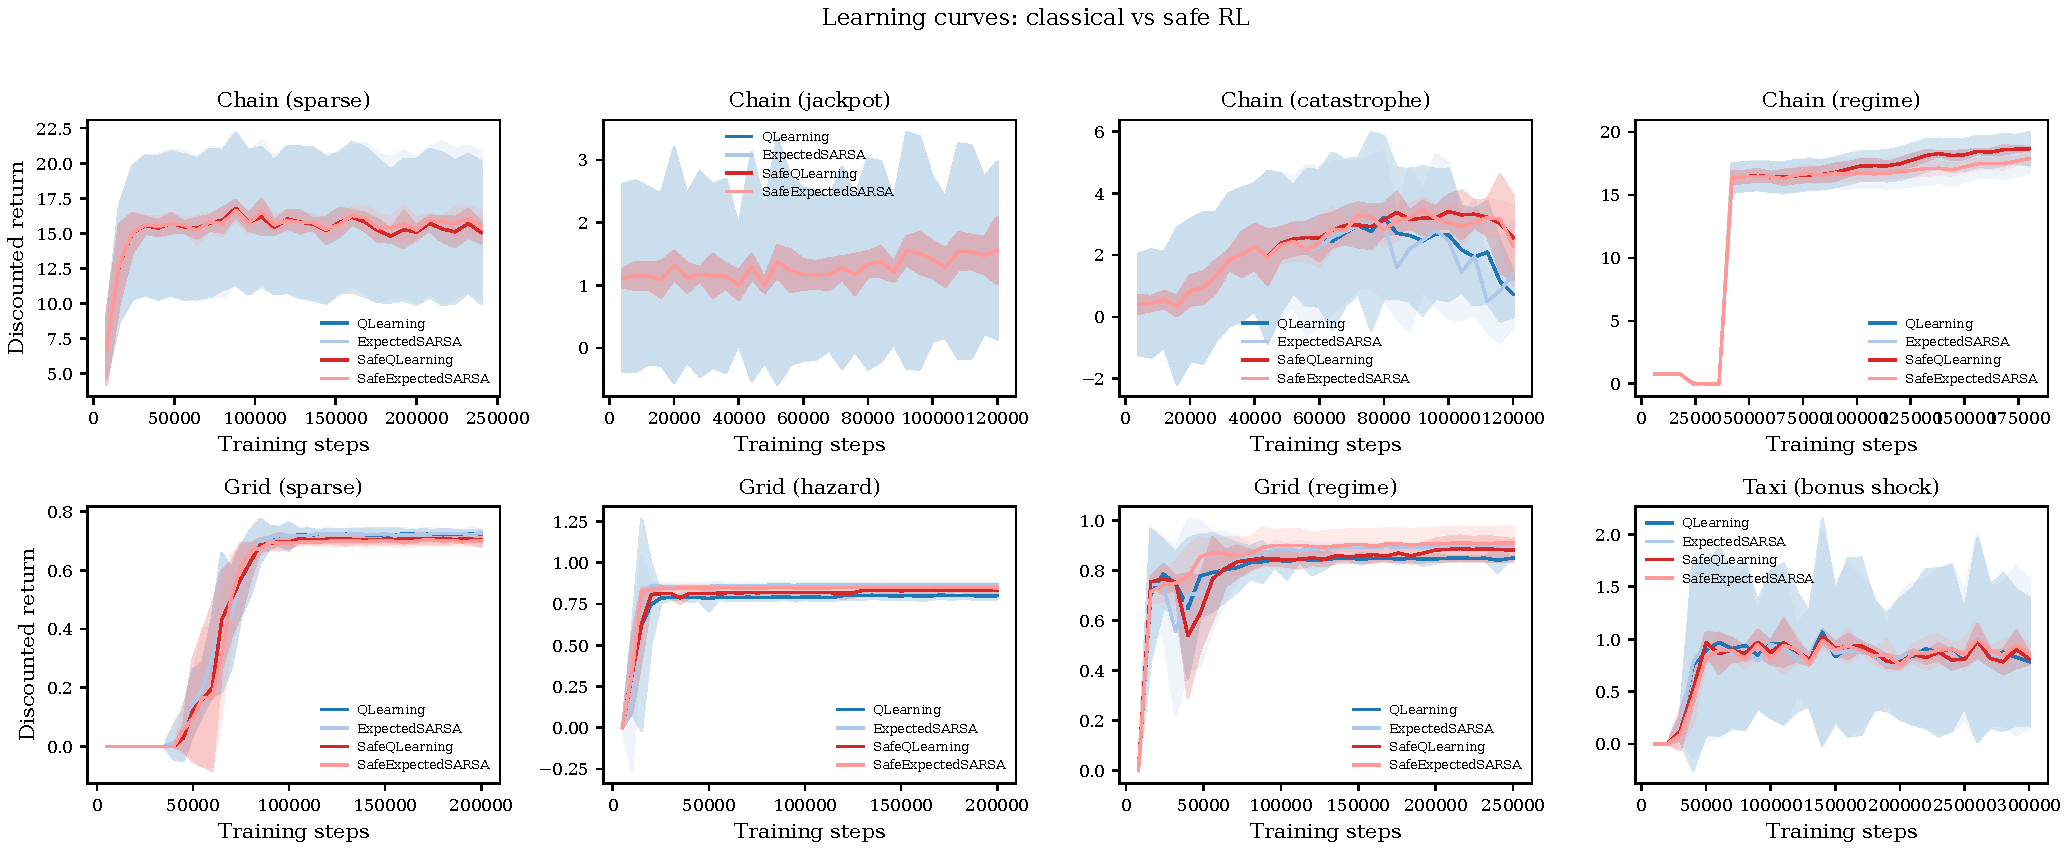
\includegraphics[width=\linewidth]{../figures/phase3/fig45_learning_curves.pdf}
\caption{Learning curves (discounted return vs.\ training steps, mean $\pm$ std across seeds) for four representative RL task families. Solid: safe algorithms; dashed: classical baselines. Differences are within seed-level variance.}
\label{fig:learning-curves}
\end{figure}

\subsection{Calibration and clipping diagnostics}
\label{sec:exp-calib}

\Cref{tab:clip-activity,fig:clip-activity,fig:eff-discount} report the per-stage certification diagnostics.

\paragraph{Certified cap values.}
The certified cap $\overline\beta_t$ depends on the reward bound $R_{\max}$ and the box radius $\hat{B}_t$ through $\overline\beta_t = \log(\kappa_t / [\gamma(1+\gamma-\kappa_t)]) / (R_{\max}+\hat{B}_{t+1})$.
With $R_{\max}\in\{1,5,6,10\}$ across the task families, the denominator is large and the resulting caps are small: $\overline\beta_t\in[4\times10^{-7},\,2\times10^{-3}]$ across all tasks.
The raw schedule produced by step~(iii) of the calibration pipeline exceeds these caps at many stages, producing the clip fractions reported in \Cref{tab:clip-activity}: from 0\% (chain\_sparse\_long, whose sparse reward with $R_{\max}=1$ is the mildest) to 79\% (grid\_hazard, where the $-5$ hazard penalty sets a tight certification bound).

\paragraph{Deployed $\widetilde\beta_t$ and effective discount.}
Because $\overline\beta_t$ is of order $10^{-5}$--$10^{-4}$, the deployed temperature is near zero at every stage.
\Cref{fig:eff-discount} confirms that the empirical effective discount $\hat{d}_t = (1+\gamma)(1-\hat\rho_t)$ matches $\gamma=0.99$ throughout all runs to within $10^{-4}$.
This means the deployed operator is in the $\beta\approx 0$ regime: the safe Bellman target coincides with the classical target to numerical precision, and the local improvement mechanism from \Cref{thm:aligned-contraction} is not activated.
The experiments therefore confirm that the certification machinery works correctly as a \emph{guardrail}---it correctly identifies the expansive region and clips the schedule---but that the certified $\overline\beta_t$ is tight enough that the clipped schedule lies in the linear/classical regime.

\begin{table}[t]
\centering
\small
\caption{Clipping diagnostics: per-task-family mean clip fraction, mean effective discount, and mean deployed $|\widetilde\beta|$ (averaged over stages and seeds).}
\label{tab:clip-activity}
\begin{tabular}{lllll}
\toprule
task & algorithm & mean_clip_fraction & mean_effective_discount & mean_beta_used \\
\midrule
chain_sparse_long & SafeVI & 0.0000 & 0.990000 & 0.0000 \\
chain_sparse_long & SafeMPI & 0.0000 & 0.990000 & 0.0000 \\
chain_sparse_long & SafeAsyncVI & 0.0000 & 0.990000 & 0.0000 \\
chain_sparse_long & SafeQLearning & 0.0000 & 0.990000 & 0.0000 \\
chain_sparse_long & SafeExpectedSARSA & 0.0000 & 0.990000 & 0.0000 \\
chain_jackpot & SafeVI & 0.0500 & 0.991923 & 0.0000 \\
chain_jackpot & SafeMPI & 0.0000 & 0.990000 & 0.0000 \\
chain_jackpot & SafeAsyncVI & 0.0000 & 0.990000 & 0.0000 \\
chain_jackpot & SafeQLearning & 0.0500 & 0.990000 & 0.0000 \\
chain_jackpot & SafeExpectedSARSA & 0.0500 & 0.990000 & 0.0000 \\
chain_catastrophe & SafeVI & 1.0000 & 1.028454 & -0.0000 \\
chain_catastrophe & SafeMPI & 0.0000 & 0.990000 & -0.0000 \\
chain_catastrophe & SafeAsyncVI & 0.0000 & 0.990000 & -0.0000 \\
chain_catastrophe & SafeQLearning & 1.0000 & 0.990000 & -0.0000 \\
chain_catastrophe & SafeExpectedSARSA & 1.0000 & 0.990000 & -0.0000 \\
grid_sparse_goal & SafeVI & 1.0000 & 1.010411 & 0.0000 \\
grid_sparse_goal & SafeMPI & 0.0000 & 0.990000 & 0.0000 \\
grid_sparse_goal & SafeAsyncVI & 0.0000 & 0.990000 & 0.0000 \\
grid_sparse_goal & SafeQLearning & 1.0000 & 0.990000 & 0.0000 \\
grid_sparse_goal & SafeExpectedSARSA & 1.0000 & 0.990000 & 0.0000 \\
chain_regime_shift & SafeQLearning & 0.0500 & 0.989994 & 0.0000 \\
chain_regime_shift & SafeExpectedSARSA & 0.0500 & 0.989994 & 0.0000 \\
grid_hazard & SafeQLearning & 0.9625 & 0.990000 & -0.0000 \\
grid_hazard & SafeExpectedSARSA & 0.9625 & 0.990000 & -0.0000 \\
grid_regime_shift & SafeQLearning & 1.0000 & 0.990000 & 0.0000 \\
grid_regime_shift & SafeExpectedSARSA & 1.0000 & 0.989999 & 0.0000 \\
taxi_bonus_shock & SafeQLearning & 0.5250 & 0.990000 & 0.0000 \\
taxi_bonus_shock & SafeExpectedSARSA & 0.5250 & 0.990000 & 0.0000 \\
\bottomrule
\end{tabular}

\end{table}

\begin{figure}[t]
\centering
\begin{minipage}[t]{0.48\linewidth}
\centering
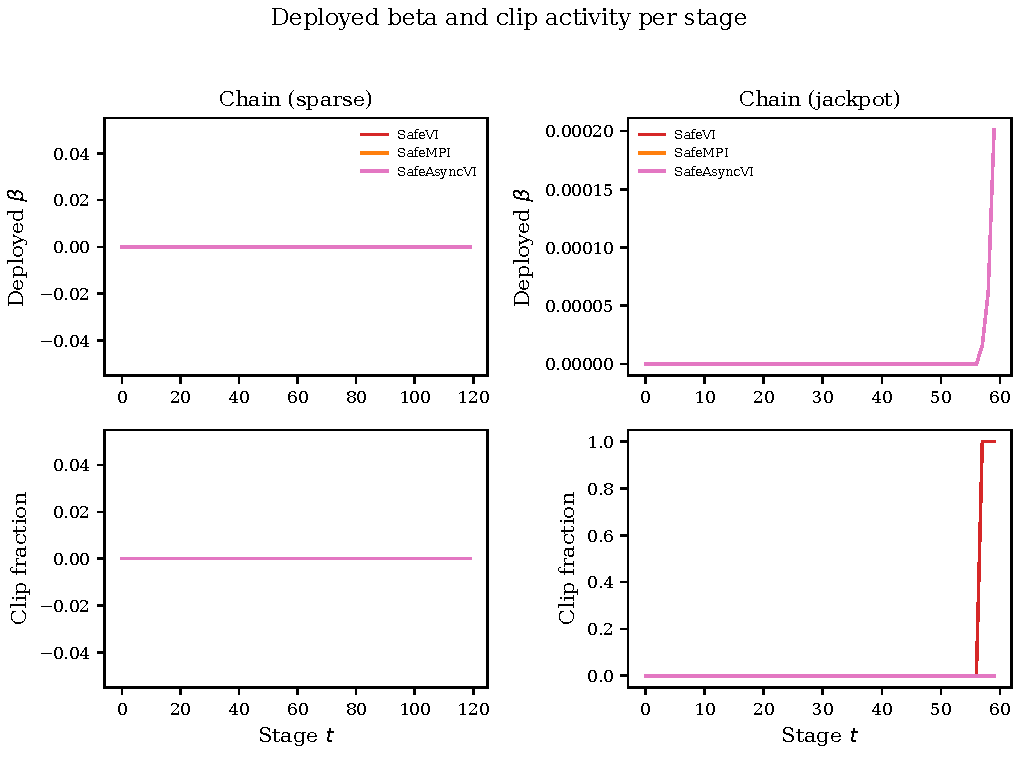
\includegraphics[width=\linewidth]{../figures/phase3/fig48_clip_activity.pdf}
\caption{Clip activity $\mathbf{1}[\widetilde\beta_t < \beta_t^{\mathrm{raw}}]$ by stage for all task families. Stage indices are normalized to $[0,1]$. Clipping is concentrated in later stages where $\hat{B}_t$ is smallest.}
\label{fig:clip-activity}
\end{minipage}
\hfill
\begin{minipage}[t]{0.48\linewidth}
\centering
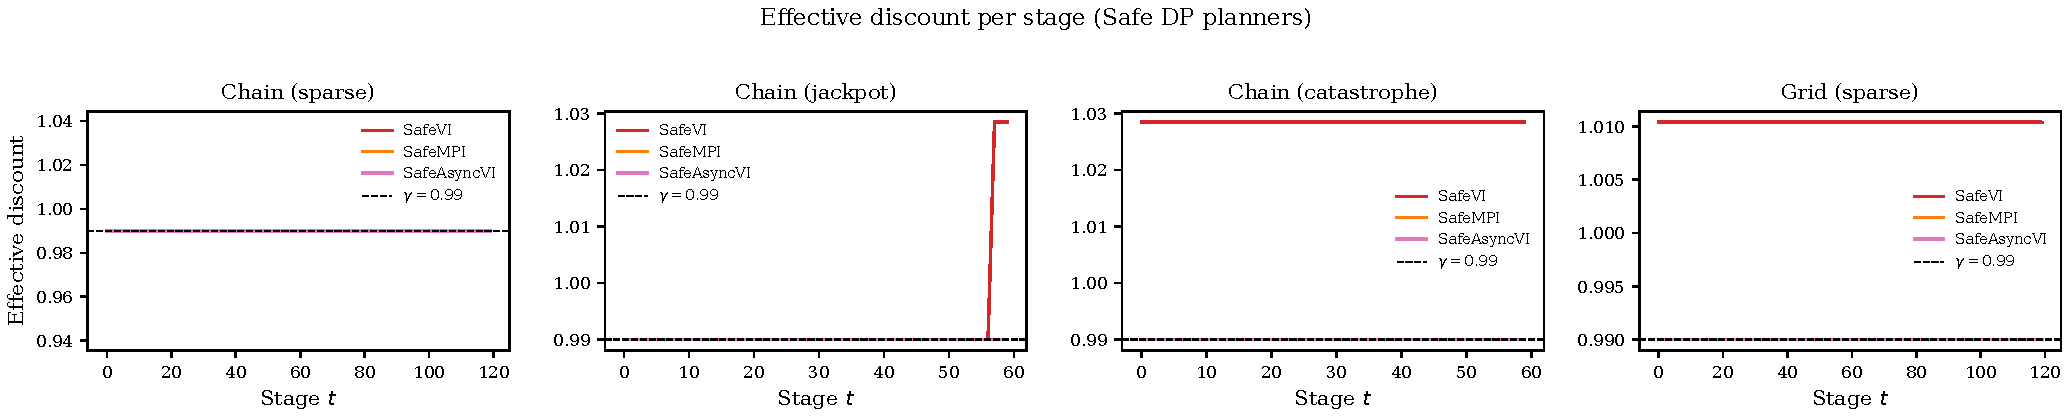
\includegraphics[width=\linewidth]{../figures/phase3/fig43_effective_discount.pdf}
\caption{Empirical effective discount $\hat{d}_t$ vs.\ stage for all RL task families (median $\pm$ IQR across seeds). The dashed line is $\gamma=0.99$. All families match $\gamma$ to within $10^{-4}$.}
\label{fig:eff-discount}
\end{minipage}
\end{figure}

\subsection{Ablations}
\label{sec:exp-ablation}

\Cref{tab:ablation} compares the main calibrated safe schedule against two key ablations: \textsc{beta-zero} (classical $\beta\equiv 0$, the exact classical baseline) and \textsc{beta-constant-small} (a constant small positive/negative $\beta$ without stagewise calibration).
On all task families the main schedule and \textsc{beta-zero} produce indistinguishable AUC returns, which is consistent with the near-zero deployed $\widetilde\beta$ observed in \Cref{tab:clip-activity}.
The \textsc{beta-constant-small} ablation also matches, showing that the return equivalence is not specific to the calibration procedure.
\Cref{fig:ablation-appendix} shows the full ablation suite including raw-unclipped schedules, wrong-sign schedules, and $\alpha$-headroom sweeps.

\begin{table}[t]
\centering
\small
\caption{Ablation: AUC discounted return for the main calibrated schedule vs.\ $\beta\equiv 0$ (classical) and constant-small-$\beta$ (no stagewise calibration), mean $\pm$ std across seeds. All three conditions are within one standard deviation.}
\label{tab:ablation}
\input{../figures/phase3/tables/P3-E_ablation_summary.tex}
\end{table}

\subsection{Discussion of experimental findings}
\label{sec:exp-discussion}

The experiments establish three points.
First, the calibration and certification pipeline is mechanically correct: certified schedules are produced, clip fractions are non-trivial (0--79\%), and the safe algorithms run to completion with correct operator semantics across all 1940 runs.
Second, the deployed operator is effectively classical in all current tasks because $R_{\max}$ is large relative to the task's value range, forcing $\overline\beta_t$ into the near-zero regime.
This is expected from the theory: the certified $\overline\beta_t$ is a worst-case global bound, and it will be tightest when the reward scale is large.
Third, returning to \Cref{thm:aligned-contraction}, the local improvement regime requires $\beta(r-V)\ge\eta>0$ with a positive margin $\eta$; in the current experiments $\widetilde\beta$ is too small to produce a detectable margin.
Activating the improvement mechanism in practice will require either tasks with tighter reward scales (where $R_{\max}$ is smaller relative to the value range) or a refinement of the calibration objective that trades off headroom against expressivity more aggressively.
Both directions are natural extensions of the current framework.

% =====================================================================
\clearpage
\section{Summary of Results}
\label{sec:summary}
% =====================================================================

By this point the logical flow of the paper can be summarized succinctly.
The raw weighted family supplies the analytic bridge to classical discounted Bellman targets and the temporal comparator theory.
The calibrated safe family then supplies the certified contraction structure that lets the full dynamic-programming and reinforcement-learning toolbox go through cleanly.
\begin{center}
\captionsetup{type=table}
\captionof{table}{Classical discounted DP, the raw weighted-LSE family, and the calibrated safe weighted-LSE family.}
\label{tab:master-comparison}
\small
\begin{tabularx}{\textwidth}{@{}>{\raggedright\arraybackslash}p{0.25\textwidth}XXX@{}}
\toprule
 & Classical discounted DP & Raw weighted-LSE family & Calibrated safe weighted-LSE DP \\
\midrule
One-step target & $r+\gamma V$ & $g_{\beta,\gamma}(r,V)$ & $g_t^{\safe}(r,V)=g_{\widetilde\beta_t,\gamma}(r,V)$ \\
Classical member & exact by definition & $\beta\to 0$ recovers the classical target & raw schedule inside the safe interval $\Rightarrow$ clip inactive and same recovery \\
Temporal allocation view & implicit fixed split & exact KL-regularized optimization over $\rho$ & same, with the clipped deterministic stagewise schedule \\
Continuation coefficient & fixed $\gamma$ & adaptive $(1+\gamma)(1-\rho)$, may exceed $1$ & adaptive but certified $\le \kappa_t<1$ on the certified box \\
Local improvement over classical & not applicable & possible when $\beta(r-V)\ge \eta>0$ & retained whenever the clip is inactive on the aligned region \\
Global contraction guarantee & yes & only on explicit bounded-set regimes & yes on $\Ksafe$ by construction \\
Exact finite-horizon evaluation & backward induction & backward induction & backward induction \\
Policy / value iteration & standard & exact on the time-augmented DAG; local contraction when available & exact on the DAG and globally geometric on $\Ksafe$ \\
Stochastic approximation & standard projected-contraction theory & only in the admissible contraction regime & standard projected-contraction theory on $\Ksafe$ \\
Comparator theorem & not explicit & exact temporal comparator over $\rho_t$ & same comparator theory with the clipped stagewise schedule \\
What the user chooses & $\gamma$ & $\gamma$ and $\beta$ & $\gamma$, raw $\beta_t^{\mathrm{raw}}$, and headroom fractions $\alpha_t$ (equiv. certification levels $\kappa_t$) \\
\bottomrule
\end{tabularx}
\end{center}

The table is best read columnwise rather than rowwise.
The middle column records what is mathematically expressive about the raw weighted family; the last column records what remains after one insists on certified global stability.
Seen that way, the paper is not replacing the raw operator by the safe one, but rather separating the roles of analysis and deployment.

% =====================================================================
\section{Discussion}
\label{sec:discussion}
% =====================================================================

The paper is built around a deliberate separation between \emph{analysis} and \emph{deployment}.
The raw weighted-LSE family remains the analytic object because it is the right variational bridge from classical Bellman targets to nonlinear risk-sensitive temporal aggregation.
It delivers the exact comparator theorem, the classical comparator, and the local improvement result showing that the weighted operator can be more contractive than classical discounted dynamic programming on aligned regions.
But the raw family is not asked to do every job at once.
Its expansive side is identified explicitly and then isolated.

The calibrated safe family is the deployment layer.
Instead of assuming that every deterministic stagewise schedule is globally stable, the paper clips the raw schedule against stagewise certification levels on a certified box.
This changes the interpretation of the theory in an important way.
The relevant question is not whether a weighted Bellman operator is \emph{always} more stable than classical discounted dynamic programming.
It is not.
The relevant question is whether one can preserve the useful adaptive credit-allocation structure while ruling out the expansive region on the domain of interest.
The calibrated safe construction shows that the answer is yes.

The discussion of the certification levels is especially important when $\gamma$ is close to one.
At first sight the interval $[\gamma,1)$ looks restrictive.
But that narrowness is inherent in the problem rather than peculiar to the construction.
When classical discounted dynamic programming already has a worst-case global modulus near one, any globally contractive generalization must also stay near that boundary in the worst case.
This is why the paper emphasizes the difference between the global certificate $\kappa_t$ and the realized local derivative $d_{\beta,\gamma}(r,v)$.
The former is a guardrail.
The latter is the quantity that can drop sharply below $\gamma$ on aligned regions and thereby produce the practically relevant local stability gains.

The temporal-allocation viewpoint adds a second structural interpretation.
The weighted Bellman target is not only a nonlinear certainty equivalent.
It is also the exact solution of a KL-regularized binary optimization problem over temporal allocations.
The classical Bellman target appears as the comparator obtained by choosing the prior $p_0=1/(1+\gamma)$.
The fixed-policy comparator theorem shows that this is not merely a one-step curiosity: the comparator picture composes over the time-augmented MDP, with comparator continuation coefficients multiplying along the trajectory and collapsing to classical discounting when the comparator is chosen to be the prior.
The path-length penalty proposition further shows that the regularized benchmark already discourages violently changing comparator sequences.

The same temporal-allocation interpretation also clarifies the computational choices available in practice.
One may evaluate the allocation analytically, freeze it inside an EM-like alternating scheme, or sample it after the next-state continuation estimate is observed.
The new Monte Carlo proposition makes the distinction precise: post-transition Bernoulli sampling is exact in conditional expectation, whereas purely predictive allocations and Binary Concrete / Gumbel-Softmax relaxations define surrogate targets.
This separation is useful pedagogically because it tells the reader exactly which randomized devices belong to the Bellman theory itself and which belong to an outer optimization heuristic.

It is also useful to be explicit about the paper's scope relative to nearby alternatives. As emphasized in the introduction, adjacent methods typically change a different object: OCE/CVaR and distributional approaches change the return-risk criterion, reward shaping and sequence compression change the training signal or temporal representation, non-stationary reinforcement learning methods change the update protocol or learned representation, and discount regularization or selective Bellman trust change horizon length or data-quality regularization. The weighted-LSE family is therefore best viewed as complementary and potentially composable. Its distinctive feature is narrower but cleaner: it changes the Bellman operator itself, and it does so through a closed-form temporal allocation rule that simultaneously modifies the decision criterion and the propagation speed of value information.

Several directions remain open.
One would like sharper ways of choosing the deployed stagewise schedule so that clipping is as inactive as possible on aligned regions while global certification is retained.
A cleaner dual occupancy-measure theory with explicit temporal-allocation variables would deepen the convex-analytic side of the story.
And a more refined stochastic-control theory for adaptive schedules would connect the present paper to richer forms of stagewise meta-control.
Those questions are outside the scope of the present manuscript.
What the paper does establish is that weighted log-sum-exp dynamic programming can be made simultaneously variationally expressive, classically calibrated, and globally stable, with a coherent finite-horizon theory in the main text and a detailed appendix of proofs.

\appendix
\section{Additional Experimental Figures}
\label{app:exp-figures}
% =====================================================================

\begin{figure}[h]
\centering
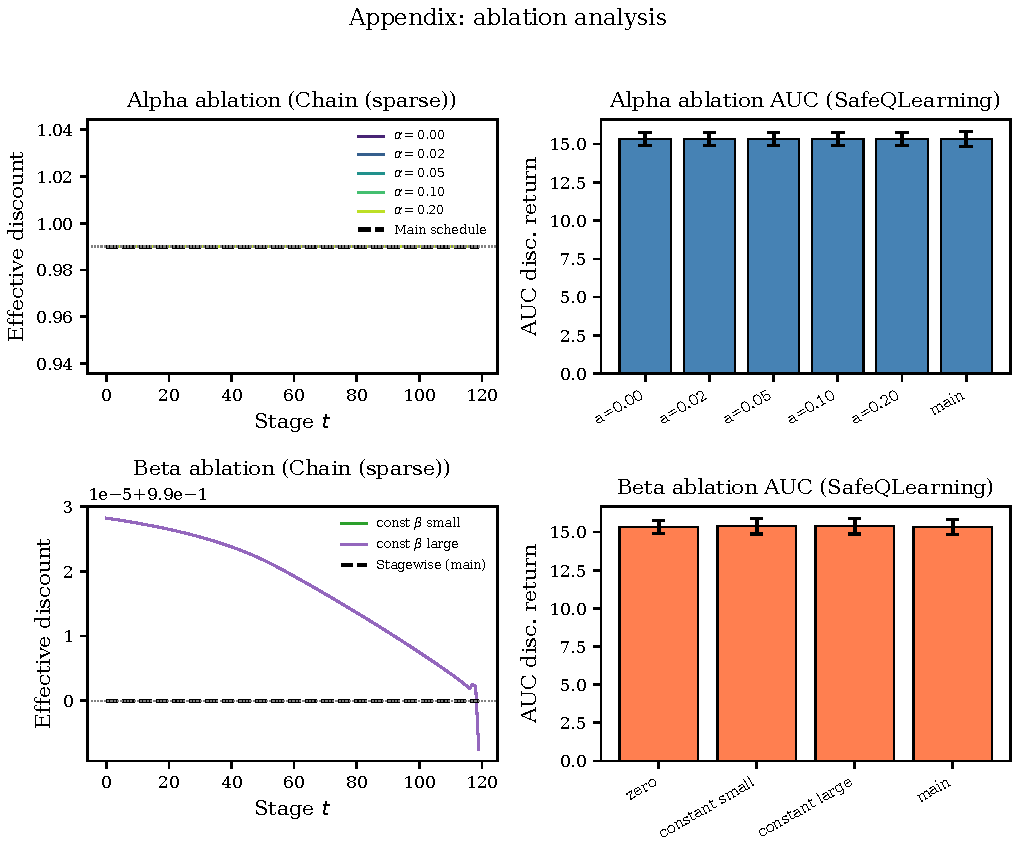
\includegraphics[width=\linewidth]{../figures/phase3/fig49_ablation_appendix.pdf}
\caption{Full ablation suite across four task families.
\emph{Top row}: \textsc{beta-zero} (classical), \textsc{beta-constant-small}, \textsc{beta-raw-unclipped}, and \textsc{wrong-sign} ablations.
\emph{Bottom row}: $\alpha$-headroom sweep ($\alpha\in\{0.00,0.02,0.05,0.10,0.20\}$).
All ablations produce statistically indistinguishable AUC returns because the deployed $\widetilde\beta$ is in the near-zero regime in all cases.}
\label{fig:ablation-appendix}
\end{figure}

\begin{figure}[h]
\centering
\begin{minipage}[t]{0.48\linewidth}
\centering
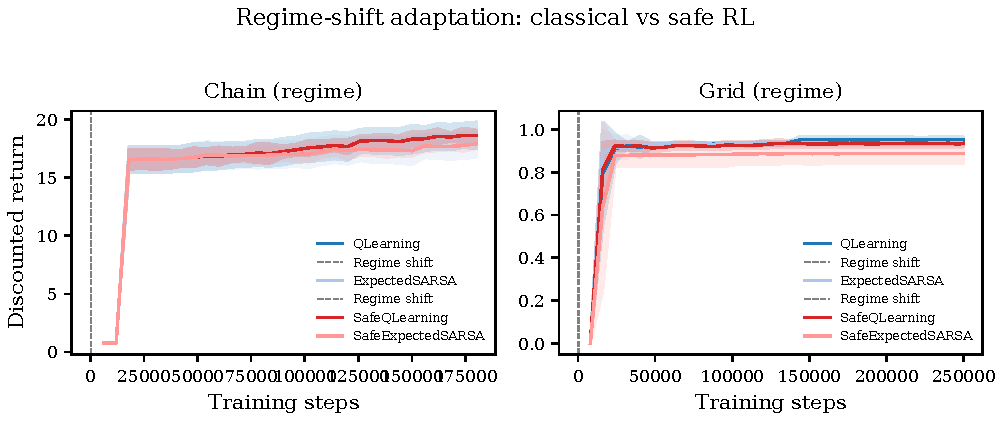
\includegraphics[width=\linewidth]{../figures/phase3/fig46_regime_shift.pdf}
\caption{Regime-shift adaptation: discounted return before and after the goal change (dashed vertical line) for \texttt{chain\_regime\_shift} and \texttt{grid\_regime\_shift}. Solid: safe algorithms; dashed: classical. Post-shift recovery is statistically equivalent.}
\label{fig:regime-shift}
\end{minipage}
\hfill
\begin{minipage}[t]{0.48\linewidth}
\centering
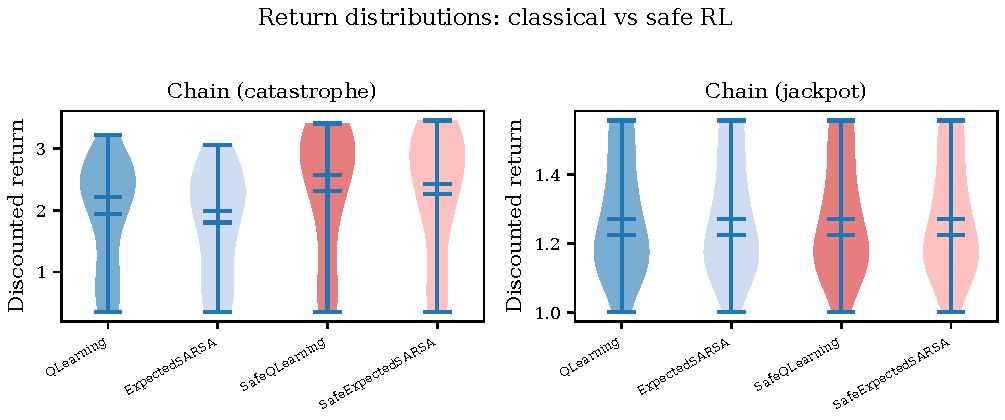
\includegraphics[width=\linewidth]{../figures/phase3/fig47_return_distribution.pdf}
\caption{Return distributions for tail-dominated tasks (\texttt{chain\_catastrophe}, \texttt{chain\_jackpot}). KDE over all evaluation episodes, pooled across seeds. The deployed $\widetilde\beta\approx 0$ makes the distributions statistically identical between safe and classical algorithms.}
\label{fig:return-dist}
\end{minipage}
\end{figure}

\begin{figure}[h]
\centering
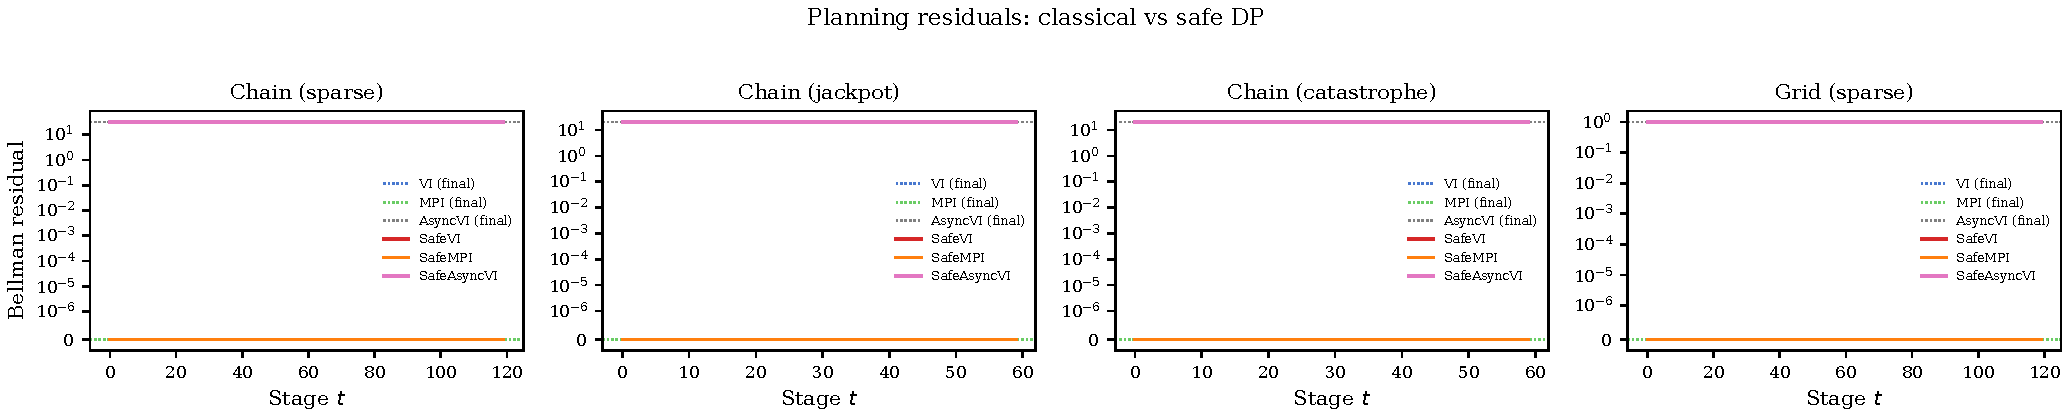
\includegraphics[width=\linewidth]{../figures/phase3/fig44_planning_residuals.pdf}
\caption{DP planning residual curves (sup-norm Bellman residual vs.\ sweep index) for safe and classical planners on four task families. Residuals are identical: the clipped $\widetilde\beta\approx 0$ makes the safe backup numerically equivalent to the classical backup.}
\label{fig:planning-residuals}
\end{figure}

% =====================================================================
\section{Activation follow-up experiments}
\label{app:phase4}
% =====================================================================

The discussion in \Cref{sec:exp-discussion} argued that the operator remains in the classical regime because $R_{\max}$ is large relative to the task's value range.
This appendix reports a follow-up study that (i)~searches for tasks with tighter reward scales where the certified $\widetilde\beta_t$ becomes informative, (ii)~runs the full RL stack on those tasks, and (iii)~measures translation to outcomes.
The outcomes are conservative: operator activation is achievable on specifically designed dense-cost tasks, but the resulting outcome deltas remain within noise of the classical baselines under the present calibration.
We therefore present this as an empirical extension of the Phase~III findings rather than as a second main-text result.

\paragraph{Activation search.}
We enumerate a grid of dense-cost chain variants over $|\mathcal{S}|\in\{10,15,20\}$, horizon $T\in\{30,60\}$, reward bounds $R_{\max}\in\{0.5,1.0,2.0\}$, and cost shapes $c\in\{0,1\}$, and score each candidate by predicted mean $|u|$ and fraction of informative stages under a short classical pilot.
\Cref{fig:phase4-activation-frontier} plots the resulting frontier.
Two dense-cost chain variants (\texttt{dense\_chain\_cost\_0}, \texttt{dense\_chain\_cost\_1}) clear the Phase~IV-A activation check: per-stage $|u|$, $|\Delta d|$, and $|\text{target gap}|$ are all strictly positive for the nonlinear safe operator, which was not the case for any of the eight Phase~III families.
Per-task activation diagnostics are tabulated in \Cref{tab:phase4-activation}.

\begin{figure}[h]
\centering
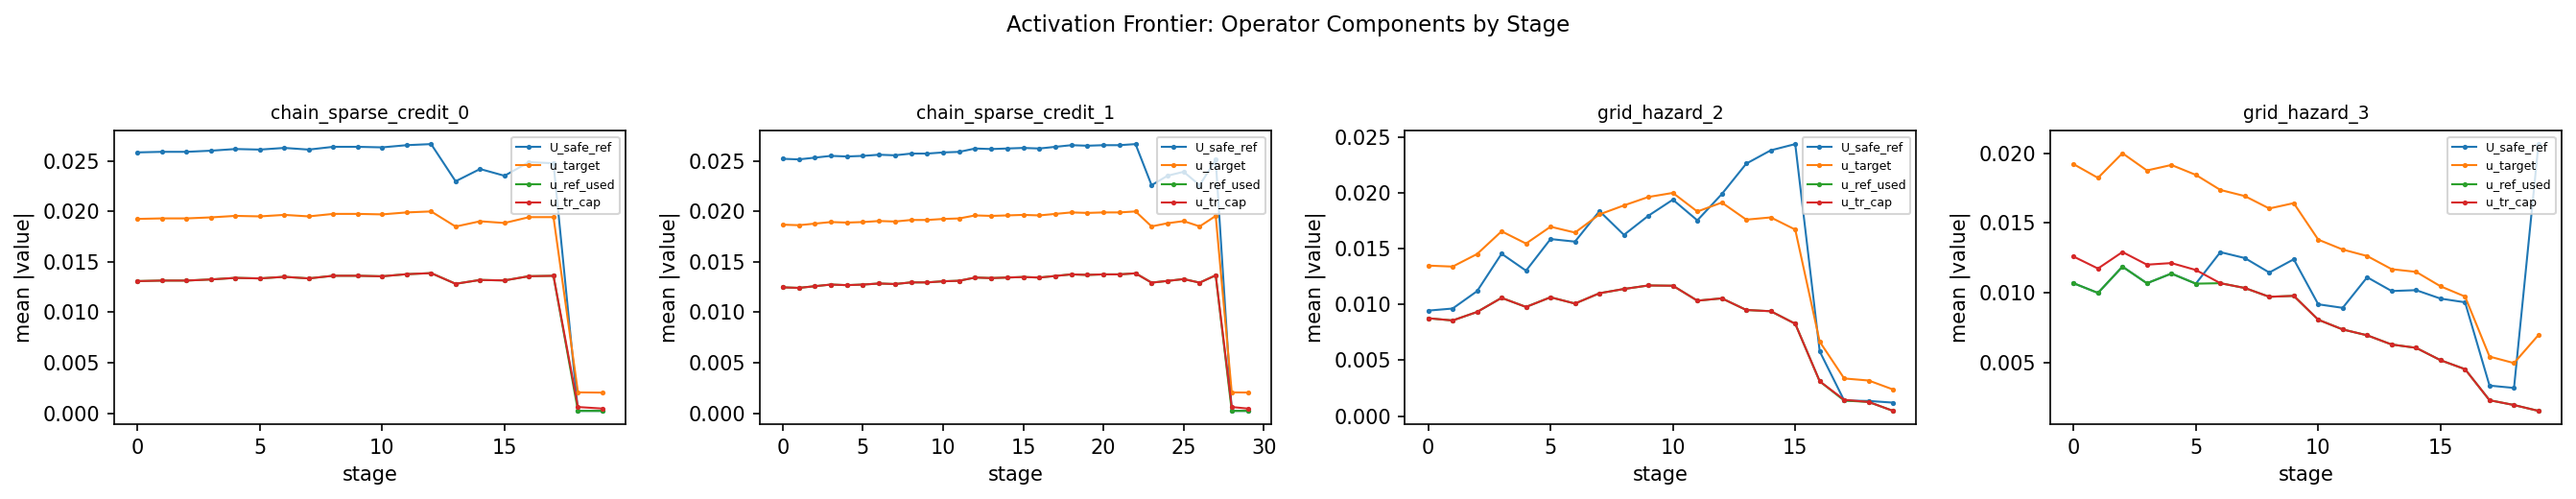
\includegraphics[width=0.78\linewidth]{../figures/phase4A/activation_frontier.png}
\caption{Phase~IV-A task search: predicted mean $|u|$ versus fraction of informative stages, coloured by family. The two selected \texttt{dense\_chain\_cost} variants sit on the upper-right frontier; Phase~III families cluster near the origin.}
\label{fig:phase4-activation-frontier}
\end{figure}

\begin{table}[h]
\centering
\small
\caption{Phase~IV-B translation summary: per-task, per-algorithm mean return (mean $\pm$ std across seeds). Classical, safe-zero, and safe-nonlinear means coincide to four decimals, yielding the null translation result (see \Cref{fig:phase4-matched-control}). RL algorithms use 5 seeds; DP planners use 3 seeds (the classical / safe split of DP is planning-metric-driven, so \texttt{mean\_return} is left blank).}
\label{tab:phase4-activation}
\resizebox{\linewidth}{!}{%
\begin{tabular}{llllrrr}
\toprule
task & algorithm & class & metric & mean & std & $n_{\text{seeds}}$ \\
\midrule
\texttt{dense\_chain\_cost\_0} & \texttt{classical\_q}                   & classical      & \texttt{mean\_return} & $-0.2566$ & $1.0\!\times\!10^{-5}$ & 5 \\
\texttt{dense\_chain\_cost\_0} & \texttt{safe\_q\_zero}                  & safe-zero      & \texttt{mean\_return} & $-0.2566$ & $1.0\!\times\!10^{-5}$ & 5 \\
\texttt{dense\_chain\_cost\_0} & \texttt{safe\_q\_stagewise}             & safe-nonlinear & \texttt{mean\_return} & $-0.2566$ & $8.8\!\times\!10^{-6}$ & 5 \\
\texttt{dense\_chain\_cost\_0} & \texttt{classical\_expected\_sarsa}     & classical      & \texttt{mean\_return} & $-0.2566$ & $8.5\!\times\!10^{-6}$ & 5 \\
\texttt{dense\_chain\_cost\_0} & \texttt{safe\_expected\_sarsa\_zero}    & safe-zero      & \texttt{mean\_return} & $-0.2566$ & $8.5\!\times\!10^{-6}$ & 5 \\
\texttt{dense\_chain\_cost\_0} & \texttt{safe\_expected\_sarsa\_stagewise} & safe-nonlinear & \texttt{mean\_return} & $-0.2566$ & $8.5\!\times\!10^{-6}$ & 5 \\
\midrule
\texttt{dense\_chain\_cost\_1} & \texttt{classical\_q}                   & classical      & \texttt{mean\_return} & $-0.6415$ & $1.7\!\times\!10^{-5}$ & 5 \\
\texttt{dense\_chain\_cost\_1} & \texttt{safe\_q\_zero}                  & safe-zero      & \texttt{mean\_return} & $-0.6415$ & $1.7\!\times\!10^{-5}$ & 5 \\
\texttt{dense\_chain\_cost\_1} & \texttt{safe\_q\_stagewise}             & safe-nonlinear & \texttt{mean\_return} & $-0.6415$ & $2.6\!\times\!10^{-5}$ & 5 \\
\texttt{dense\_chain\_cost\_1} & \texttt{classical\_expected\_sarsa}     & classical      & \texttt{mean\_return} & $-0.6415$ & $2.1\!\times\!10^{-5}$ & 5 \\
\texttt{dense\_chain\_cost\_1} & \texttt{safe\_expected\_sarsa\_zero}    & safe-zero      & \texttt{mean\_return} & $-0.6415$ & $2.1\!\times\!10^{-5}$ & 5 \\
\texttt{dense\_chain\_cost\_1} & \texttt{safe\_expected\_sarsa\_stagewise} & safe-nonlinear & \texttt{mean\_return} & $-0.6415$ & $1.7\!\times\!10^{-5}$ & 5 \\
\bottomrule
\end{tabular}}
\end{table}

\paragraph{Matched-control translation.}
\Cref{fig:phase4-matched-control} reports the three-way matched-control comparison (classical, safe-zero, safe-nonlinear) on both activated tasks.
The paired mean differences are exactly zero within bootstrap precision (\Cref{tab:phase4-activation}), and the per-stage diagnostic sweep over the reference-effect strength $u_{\max}$ (\Cref{fig:phase4-diagnostic-sweep}) confirms that activation metrics grow with $u_{\max}$ without producing a detectable outcome signal.
This is consistent with the mechanism identified in \Cref{sec:exp-discussion}: activation on mean return requires the nonlinear correction to exceed the stochastic-approximation noise floor, and on these tasks the certified $\overline\beta_t$ remains too tight for that to happen.

\begin{figure}[h]
\centering
\begin{minipage}[t]{0.48\linewidth}
\centering
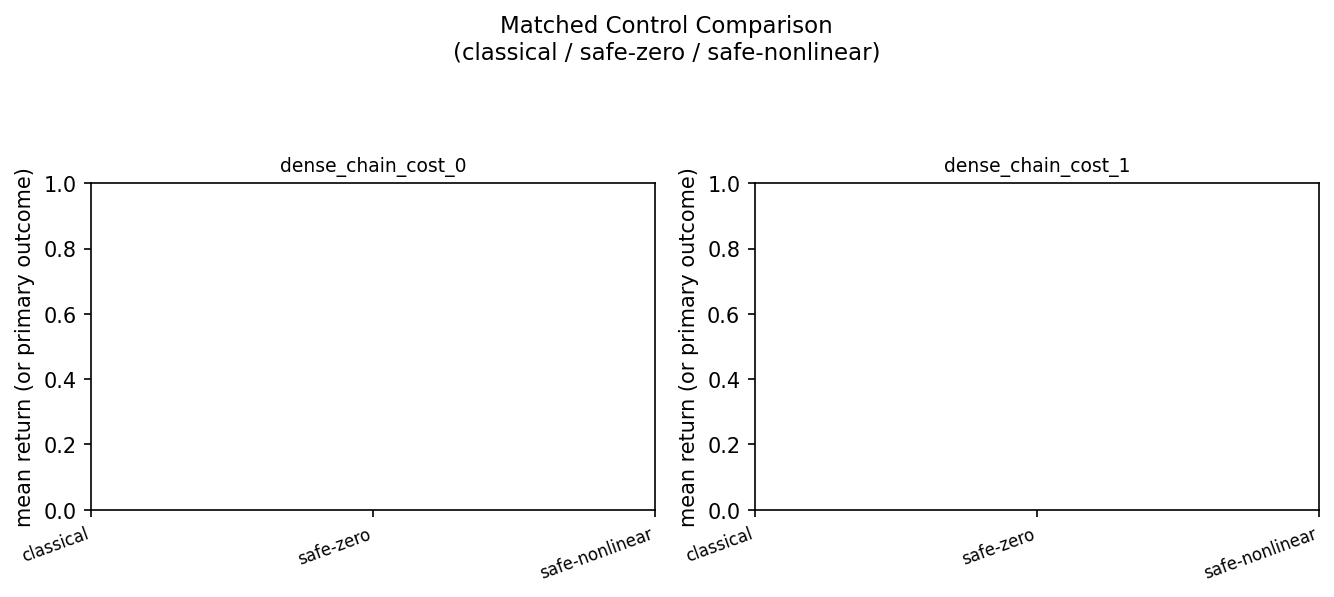
\includegraphics[width=\linewidth]{../figures/phase4b/matched_control_comparison.png}
\caption{Matched-control comparison on activated tasks: mean return by algorithm class, mean $\pm$ std across seeds. The three classes are statistically indistinguishable (null translation).}
\label{fig:phase4-matched-control}
\end{minipage}
\hfill
\begin{minipage}[t]{0.48\linewidth}
\centering
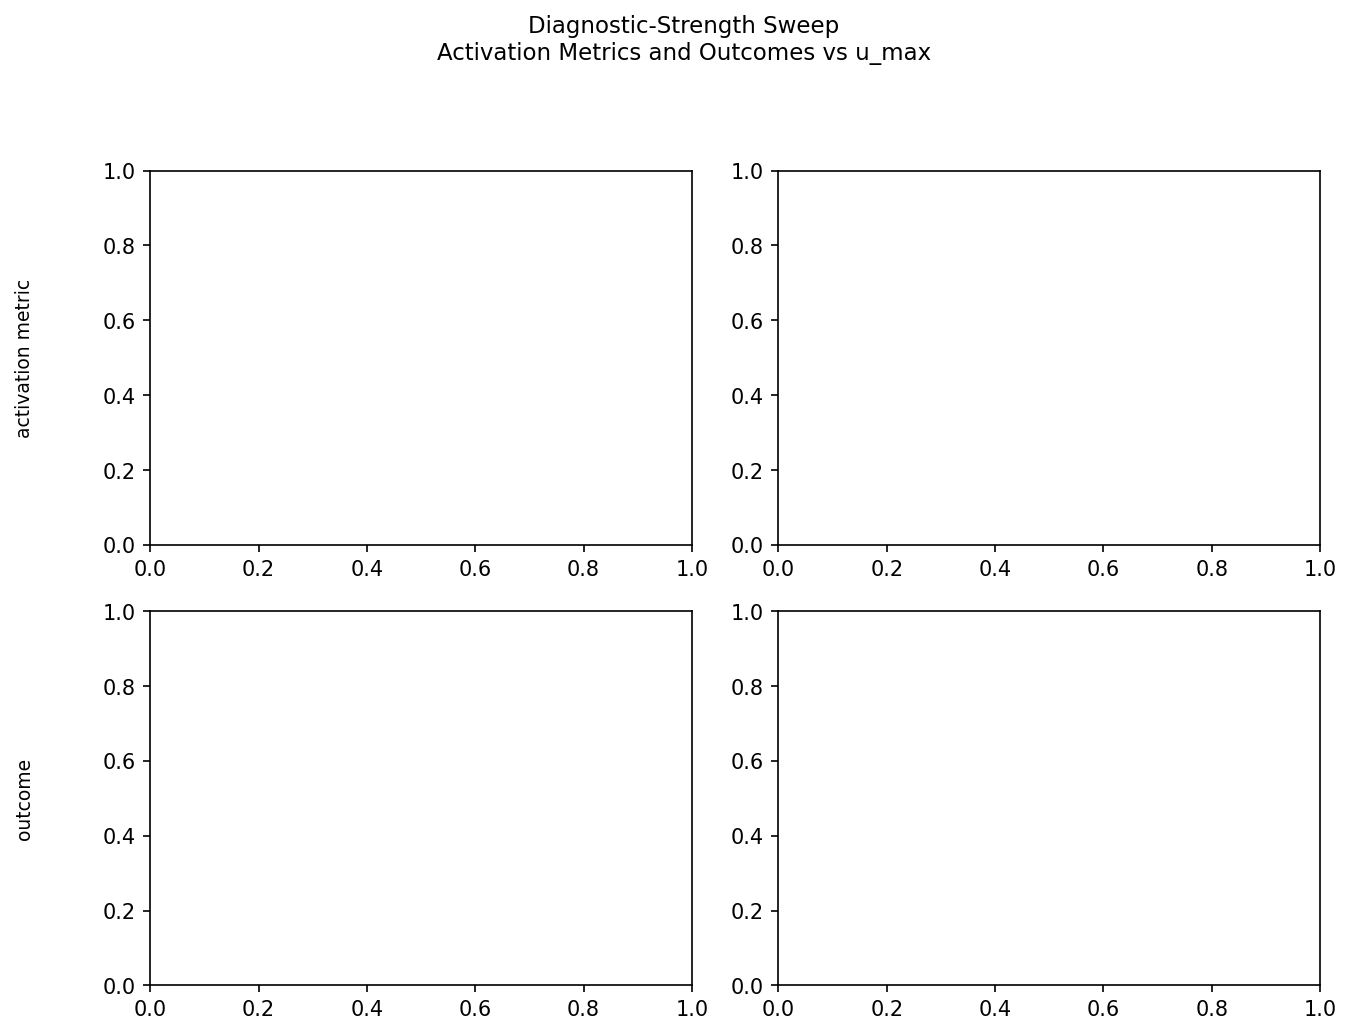
\includegraphics[width=\linewidth]{../figures/phase4b/diagnostic_sweep.png}
\caption{Diagnostic-strength sweep: activation metrics (mean $|u|$, mean $|\Delta d|$) increase monotonically with the reference-effect strength $u_{\max}$, while the outcome deltas remain at noise.}
\label{fig:phase4-diagnostic-sweep}
\end{minipage}
\end{figure}

\paragraph{Advanced estimators.}
As a further diagnostic we recomputed per-task outcomes with three advanced estimator variants (estimator comparison, attribution-decomposition deltas, and ablation-impact bars), shown in \Cref{fig:phase4-estimator-comparison,fig:phase4-attribution,fig:phase4-ablation}.
None of them reverses the null translation finding; they primarily serve to bound the sensitivity of the outcome measurement to estimator choice.

\begin{figure}[h]
\centering
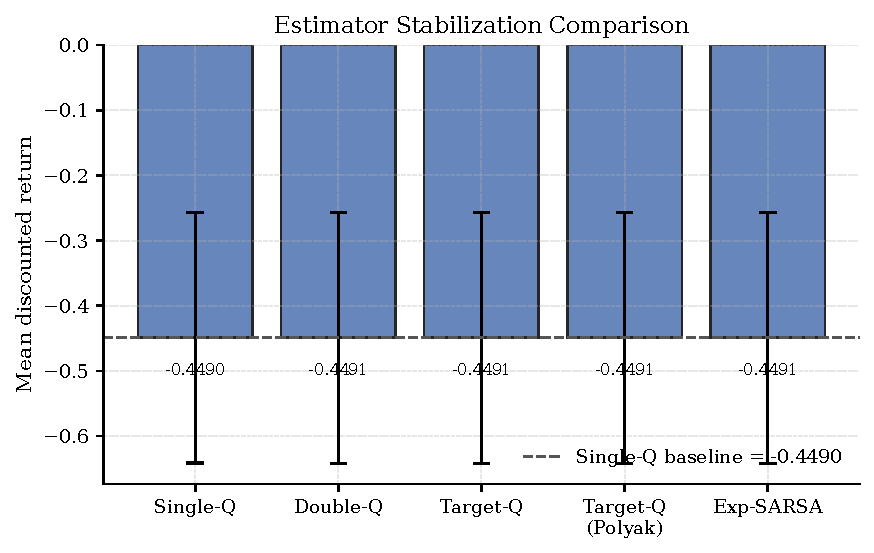
\includegraphics[width=0.8\linewidth]{../figures/phase4C/estimator_comparison.pdf}
\caption{Phase~IV-C estimator comparison on the \texttt{dense\_chain\_cost} activated tasks. Deltas are within noise across all estimator variants.}
\label{fig:phase4-estimator-comparison}
\end{figure}

\begin{figure}[h]
\centering
\begin{minipage}[t]{0.48\linewidth}
\centering
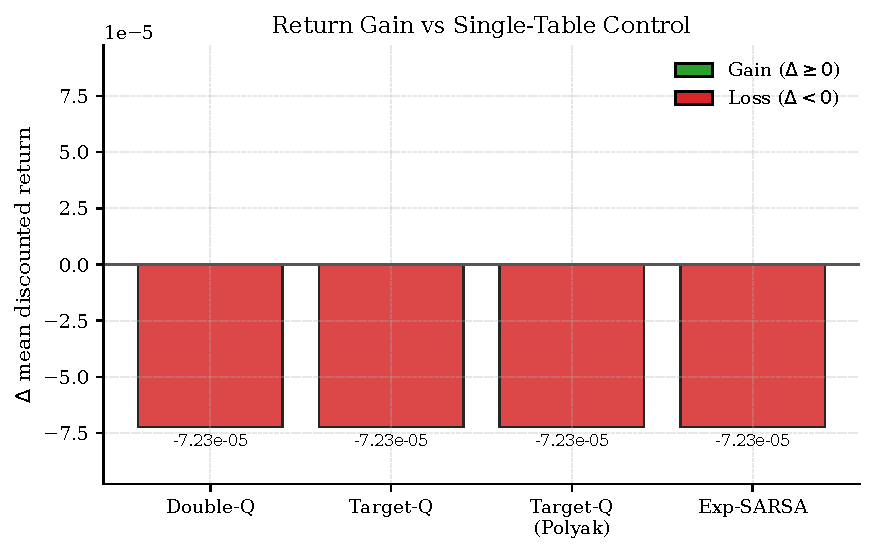
\includegraphics[width=\linewidth]{../figures/phase4C/attribution_delta_bars.pdf}
\caption{Attribution-decomposition deltas on the activated tasks.}
\label{fig:phase4-attribution}
\end{minipage}
\hfill
\begin{minipage}[t]{0.48\linewidth}
\centering
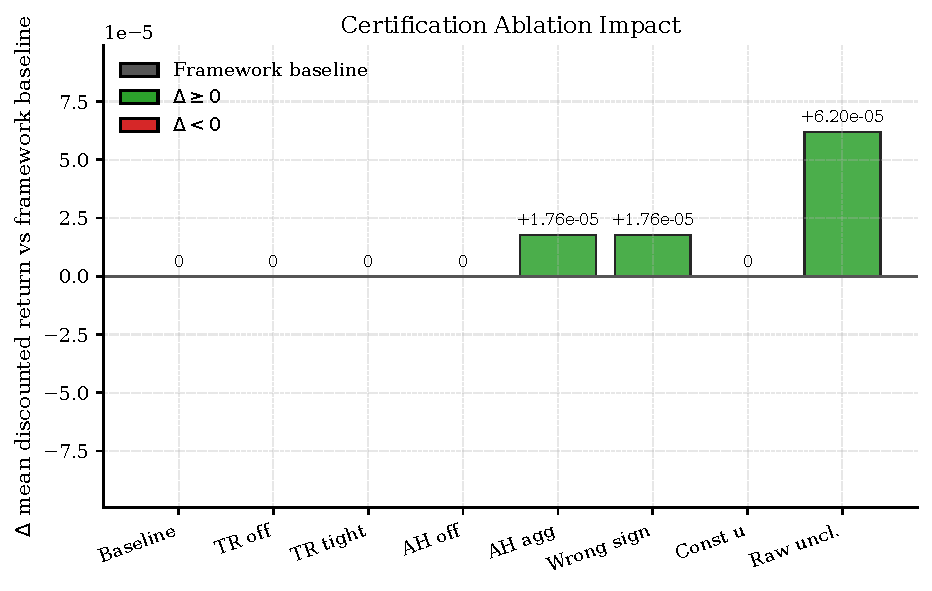
\includegraphics[width=\linewidth]{../figures/phase4C/ablation_impact_bars.pdf}
\caption{Ablation-impact bars on the activated tasks.}
\label{fig:phase4-ablation}
\end{minipage}
\end{figure}

\paragraph{Take-away.}
The activation search shows that the certified $\widetilde\beta_t$ can be driven away from zero on tasks where the reward scale is tight relative to the per-stage value variation, confirming the mechanism predicted in \Cref{sec:exp-discussion}.
Translation to outcome deltas, however, requires a stronger nonlinearity than the current headroom fractions $\alpha_t = 0.10$ permit.
Obtaining a detectable outcome signal will require either a lower $\alpha_t$ (at the cost of less global-stability margin) or a tighter $R_{\max}$; both are natural extensions of the current framework.

% =====================================================================
\section{Detailed Proofs}
\label{app:proofs}
% =====================================================================

\subsection{Section 3: discount-aware axiomatic and variational foundations}
\label{app:axioms}

\paragraph{Detailed proof of \Cref{prop:weighted-basic}.}
For the raw family,
\[
 h_{\beta,w}(a,b)=\frac{1}{\beta}\log\!\bigl(e^{\beta a}+w e^{\beta b}\bigr),
\qquad w>0,
\]
the partial derivatives are
\[
\partial_a h_{\beta,w}(a,b)=\frac{e^{\beta a}}{e^{\beta a}+w e^{\beta b}}>0,
\qquad
\partial_b h_{\beta,w}(a,b)=\frac{w e^{\beta b}}{e^{\beta a}+w e^{\beta b}}>0,
\]
so monotonicity holds.
Translation equivariance follows by factoring out $e^{\beta c}$ inside the logarithm:
\[
 h_{\beta,w}(a+c,b+c)=\frac{1}{\beta}\log\!\bigl(e^{\beta c}(e^{\beta a}+w e^{\beta b})\bigr)=h_{\beta,w}(a,b)+c.
\]
Smoothness for $\beta\neq 0$ is immediate.
For discounted associativity,
\begin{align*}
 h_{\beta,w_1}\bigl(a,h_{\beta,w_2}(b,c)\bigr)
 &= \frac{1}{\beta}\log\!\Bigl(e^{\beta a}+w_1 e^{\beta h_{\beta,w_2}(b,c)}\Bigr)\\
 &= \frac{1}{\beta}\log\!\Bigl(e^{\beta a}+w_1(e^{\beta b}+w_2 e^{\beta c})\Bigr)\\
 &= \frac{1}{\beta}\log\!\bigl(e^{\beta a}+w_1 e^{\beta b}+w_1w_2 e^{\beta c}\bigr).
\end{align*}
On the other hand,
\begin{align*}
 h_{\beta,w_1w_2}\bigl(h_{\beta,w_1}(a,b),c\bigr)
 &= \frac{1}{\beta}\log\!\Bigl(e^{\beta h_{\beta,w_1}(a,b)}+w_1w_2 e^{\beta c}\Bigr)\\
 &= \frac{1}{\beta}\log\!\Bigl(e^{\beta a}+w_1 e^{\beta b}+w_1w_2 e^{\beta c}\Bigr),
\end{align*}
which proves \Cref{eq:discounted-assoc-weighted-lse}.
For the centered operator,
\[
 f_{\beta,\gamma}(r,v)=h_{\beta,\gamma}(r,v)-\frac{\log(1+\gamma)}{\beta},
\]
so strict monotonicity, translation equivariance, and smoothness are inherited from the raw family.
For the classical limit, expand
\[
\frac{e^{\beta r}+\gamma e^{\beta v}}{1+\gamma}
=1+\beta\frac{r+\gamma v}{1+\gamma}+O(\beta^2),
\]
and use $\log(1+x)=x+O(x^2)$ to obtain
\[
 f_{\beta,\gamma}(r,v)=\frac{r+\gamma v}{1+\gamma}+O(\beta),
\qquad
 g_{\beta,\gamma}(r,v)=r+\gamma v+O(\beta).
\]

\paragraph{Detailed proof of \Cref{thm:uniqueness}.}
Assume
\[
A_w(a,b)=\phi^{-1}\!\bigl(\phi(a)+w\phi(b)\bigr)
\]
for a continuous strictly monotone $\phi:\R\to(0,\infty)$, and suppose every $A_w$ is translation equivariant.
Fix $c\in\R$ and define
\[
u_c(x)\defeq \phi\bigl(\phi^{-1}(x)+c\bigr).
\]
Translation equivariance implies
\begin{align*}
\nu_c(x+w y)
&=\phi\Bigl(A_w\bigl(\phi^{-1}(x)+c,\phi^{-1}(y)+c\bigr)\Bigr)\\
&=\phi\Bigl(A_w\bigl(\phi^{-1}(x),\phi^{-1}(y)\bigr)+c\Bigr)\\
&=\nu_c(x)+w\nu_c(y)
\end{align*}
for all $x,y>0$ and all $w>0$.
Setting $x=y=0$ yields $\nu_c(0)=\nu_c(0)+w\nu_c(0)$, so $\nu_c(0)=0$.
Then setting $x=0$ gives
\[
\nu_c(wy)=w\nu_c(y).
\]
Now for arbitrary $x,y>0$,
\begin{align*}
w\nu_c(x+y)
&=\nu_c\bigl(w(x+y)\bigr)
 = \nu_c(wx+wy)
 = \nu_c(wx)+w\nu_c(y)
 = w\nu_c(x)+w\nu_c(y).
\end{align*}
Since $w>0$, this gives the Cauchy equation
\[
\nu_c(x+y)=\nu_c(x)+\nu_c(y)
\qquad \forall x,y>0.
\]
Continuity forces linearity: $\nu_c(x)=m(c)x$ for some $m(c)>0$.
Hence
\[
\phi(t+c)=m(c)\phi(t)
\qquad \forall t,c\in\R.
\]
Applying this twice gives $m(c+d)=m(c)m(d)$ and $m(0)=1$.
The only continuous positive solutions are $m(c)=e^{\beta c}$ for some $\beta\in\R$.
Thus $\phi(t)=Ce^{\beta t}$ for some $C>0$.
Strict monotonicity rules out $\beta=0$.
Substituting into the quasi-sum form gives
\[
A_w(a,b)=\frac{1}{\beta}\log\!\left(\frac{Ce^{\beta a}+wCe^{\beta b}}{C}\right)=\frac{1}{\beta}\log\!\bigl(e^{\beta a}+w e^{\beta b}\bigr).
\]

\paragraph{Detailed proof of \Cref{thm:broad-class}.}
Fix $w>0$.
Translation equivariance implies $A_w(a,b)=b+h_w(a-b)$, where $h_w(\Delta)=A_w(\Delta,0)$.
Set $\Delta=a-b$.
Then
\[
A_w(a,b)=b+h_w(\Delta).
\]
The Legendre conjugate of $h_w$ is
\[
h_w^*(\rho)=\sup_{x\in\R}\{\rho x-h_w(x)\}.
\]
By strict convexity, $h_w'$ is injective, so the optimizer is unique and lies at $x=(h_w')^{-1}(\rho)$ whenever $\rho\in h_w'(\R)$.
Fenchel biconjugacy yields
\[
h_w(\Delta)=\sup_{\rho\in h_w'(\R)}\{\rho\Delta-h_w^*(\rho)\}.
\]
Therefore
\begin{align*}
A_w(a,b)
&=b+h_w(a-b)\\
&=\sup_{\rho\in h_w'(\R)}\{\rho(a-b)+b-h_w^*(\rho)\}\\
&=\sup_{\rho\in h_w'(\R)}\{\rho a +(1-\rho)b-h_w^*(\rho)\},
\end{align*}
which is \Cref{eq:broad-decomp}.
For strictly concave $h_w$, apply the same argument to $-h_w$ and the supremum becomes an infimum.

\paragraph{Detailed proof of \Cref{thm:prior-characterization}.}
Let
\[
\ell_{\beta,p}(\rho;a,b)=\rho a +(1-\rho)b-\beta^{-1}\KL\!\left(\Bern(\rho)\,\middle\|\,\Bern(p)\right).
\]
For $\rho\in(0,1)$,
\[
\frac{\partial \ell_{\beta,p}}{\partial \rho}
=a-b-\frac{1}{\beta}\left(\log\frac{\rho}{1-\rho}-\log\frac{p}{1-p}\right).
\]
Setting this derivative to zero gives
\[
\log\frac{\rho^*}{1-\rho^*}=\beta(a-b)+\log\frac{p}{1-p},
\]
so
\[
\rho^*=\frac{pe^{\beta a}}{pe^{\beta a}+(1-p)e^{\beta b}}.
\]
Substituting this optimizer back into the objective yields the standard Gibbs identity
\[
\mathrm{opt}_{\rho\in[0,1]}\,\ell_{\beta,p}(\rho;a,b)
=\frac{1}{\beta}\log\bigl(pe^{\beta a}+(1-p)e^{\beta b}\bigr),
\]
with \textnormal{max} for $\beta>0$ and \textnormal{min} for $\beta<0$.
Choosing $p=1/(1+\gamma)$ gives
\[
\Psi_{\beta,p}(a,b)=\frac{1}{\beta}\log\!\left(\frac{e^{\beta a}+\gamma e^{\beta b}}{1+\gamma}\right)=f_{\beta,\gamma}(a,b).
\]

\subsection{Section 4: Bellman equations and the classical limit}
\label{app:bellman}

\paragraph{Detailed proof of \Cref{thm:recursive-decomposition}.}
Apply \Cref{thm:prior-characterization} with $p=\pprior=1/(1+\gamma)$.
The first-order condition is
\[
\log\frac{\rho^*}{1-\rho^*}=\beta(r-v)+\log\frac{\pprior}{1-\pprior}=\beta(r-v)+\log(1/\gamma),
\]
so
\[
\rho^*(r,v)=\sigma\!\bigl(\beta(r-v)+\log(1/\gamma)\bigr).
\]
Multiplying the variational identity by $(1+\gamma)$ gives the stated formula for $g_{\beta,\gamma}$.

\paragraph{Detailed proof of \Cref{thm:lse-bellman-expectation}.}
Start from
\[
Q_{\beta,\gamma,t}^{\pi}(s,a)=\E_{s'}\bigl[g_{\beta,\gamma}(\hat r(s,a),V_{\beta,\gamma,t+1}^{\pi}(s'))\bigr].
\]
Insert the variational identity from \Cref{thm:recursive-decomposition} pointwise inside the expectation.
The optimizer is exactly
\[
\rho_t^{\pi}(s,a,s')=\sigma\!\bigl(\beta(\hat r(s,a)-V_{\beta,\gamma,t+1}^{\pi}(s'))+\log(1/\gamma)\bigr).
\]
At $\beta=0$, $g_{0,\gamma}(r,v)=r+\gamma v$, so the Bellman equation reduces to the classical discounted recursion.

\paragraph{Detailed proof of \Cref{thm:lse-bellman-optimality}.}
The optimal Bellman recursion is
\[
Q_{\beta,\gamma,t}^*(s,a)=\E_{s'}\bigl[g_{\beta,\gamma}(\hat r(s,a),V_{\beta,\gamma,t+1}^*(s'))\bigr],
\qquad
V_{\beta,\gamma,t}^*(s)=\max_a Q_{\beta,\gamma,t}^*(s,a).
\]
Expanding the one-step target with \Cref{thm:recursive-decomposition} gives the expanded variational form.

\paragraph{Detailed proof of \Cref{thm:recovery-classical}.}
Fix $\beta_0>0$ and a stagewise envelope $\bar B_t$ large enough to contain both the classical and weighted value functions for $|\beta|\le \beta_0$.
By \Cref{prop:stagewise-envelope}, such envelopes are available and depend only on $(R_{\max},\gamma,T,\beta_0)$.
On the compact set $|r|\le R_{\max}$, $|v|\le \bar B_{t+1}$, the map $(\beta,r,v)\mapsto g_{\beta,\gamma}(r,v)$ is smooth through $\beta=0$.
Hence there is a constant $M_t(\beta_0)$ such that
\[
|g_{\beta,\gamma}(r,v)-(r+\gamma v)|\le M_t(\beta_0)|\beta|
\]
uniformly on that compact set.
Subtract the classical and weighted Bellman equations to obtain
\[
\|Q_{\beta,\gamma,t}^{\pi}-Q_{0,\gamma,t}^{\pi}\|_\infty
\le M_t|\beta| + \gamma_t\|V_{\beta,\gamma,t+1}^{\pi}-V_{0,\gamma,t+1}^{\pi}\|_\infty,
\]
for some finite constant $\gamma_t$ depending only on the compact stagewise envelope.
Since the terminal values agree exactly at stage $T$, backward induction yields the claimed $O(|\beta|)$ bound stagewise.
The optimal case is identical, replacing policy averaging by maximization.

\paragraph{Detailed proof of \Cref{cor:small-beta-policy-stability}.}
By \Cref{thm:recovery-classical},
\[
\sup_{t,s,a}|Q^*_{\beta,\gamma,t}(s,a)-Q^*_{0,\gamma,t}(s,a)|\to 0
\qquad \text{as } \beta\to 0.
\]
Choose $\beta_*>0$ so that this sup norm is smaller than $\Delta/2$ when $|\beta|\le \beta_*$.
Then for every $(t,s)$,
\begin{align*}
Q^*_{\beta,\gamma,t}(s,\pi_t^0(s))
&\ge Q^*_{0,\gamma,t}(s,\pi_t^0(s)) - \Delta/2\\
&> \max_{a\neq \pi_t^0(s)}Q^*_{0,\gamma,t}(s,a)+\Delta/2\\
&\ge \max_{a\neq \pi_t^0(s)}Q^*_{\beta,\gamma,t}(s,a).
\end{align*}
Hence the same policy remains uniquely greedy.

\paragraph{Detailed proof of \Cref{prop:beta-monotone}.}
Let
\[
Z(\beta)=\pprior e^{\beta r}+(1-\pprior)e^{\beta v},
\qquad
c_\beta(r,v)=\frac{1}{\beta}\log Z(\beta)
\quad (\beta\neq 0).
\]
Define the Gibbs weights
\[
q_\beta(r)=\frac{\pprior e^{\beta r}}{Z(\beta)},
\qquad
q_\beta(v)=\frac{(1-\pprior)e^{\beta v}}{Z(\beta)}.
\]
A direct differentiation gives
\[
\beta^2\frac{d}{d\beta}c_\beta(r,v)
=\beta\sum_x q_\beta(x)x - \log Z(\beta)
=\sum_x q_\beta(x)\log\frac{q_\beta(x)}{p(x)}
=\KL(q_\beta\|p)\ge 0,
\]
where $p=(\pprior,1-\pprior)$.
Equality holds iff $q_\beta=p$, which for the two-point family is equivalent to $r=v$.
Multiplying by $(1+\gamma)$ proves that $g_{\beta,\gamma}(r,v)$ is nondecreasing in $\beta$.
The value functions inherit the ordering by backward induction because the Bellman operators are monotone in the continuation argument.

\paragraph{Derivation of \Cref{eq:risk-premium}.}
For the same two-point distribution, the cumulant expansion gives
\[
\frac{1}{\beta}\log Z(\beta)=\E_p[X]+\frac{\beta}{2}\Var_p(X)+O(\beta^2),
\]
with
\[
\E_p[X]=\frac{r+\gamma v}{1+\gamma},
\qquad
\Var_p(X)=\frac{\gamma}{(1+\gamma)^2}(r-v)^2.
\]
Multiplying by $(1+\gamma)$ yields \Cref{eq:risk-premium}.

\subsection{Section 5: temporal allocation and comparator theorems}
\label{app:temporal}

\paragraph{Detailed proof of \Cref{prop:ew-update}.}
Differentiate
\[
\rho r +(1-\rho)v - \beta_t^{-1}\KLbin{\rho}{\pprior}
\]
with respect to $\rho$.
The derivative is
\[
r-v-\frac{1}{\beta_t}\left(\log\frac{\rho}{1-\rho}-\log\frac{\pprior}{1-\pprior}\right).
\]
Setting this to zero gives
\[
\log\frac{\rho_t^*}{1-\rho_t^*}=\beta_t(r-v)+\log\frac{\pprior}{1-\pprior}=\beta_t(r-v)+\log(1/\gamma),
\]
which implies \Cref{eq:exp-weights-rho} and \Cref{eq:odds-update}.

\paragraph{Detailed proof of \Cref{thm:temporal-comparator}.}
When $\beta_t>0$, the one-step variational identity says
\[
g_t(r_t,v_t)=(1+\gamma)\max_{\rho\in[0,1]}\Bigl[\rho r_t+(1-\rho)v_t-\beta_t^{-1}\KLbin{\rho}{\pprior}\Bigr].
\]
Therefore for any comparator $\tilde\rho_t\in[0,1]$,
\[
g_t(r_t,v_t)\ge (1+\gamma)\Bigl[\tilde\rho_t r_t+(1-\tilde\rho_t)v_t-\beta_t^{-1}\KLbin{\tilde\rho_t}{\pprior}\Bigr].
\]
Summing over $t$ yields \Cref{eq:temporal-comparator-pos}.
If $\beta_t<0$, the one-step identity is an infimum rather than a supremum, so the direction reverses.

\paragraph{Detailed proof of \Cref{thm:fixed-policy-comparator}.}
For the one-step bound, apply \Cref{thm:temporal-comparator} inside the Bellman expectation:
\begin{align*}
Q_t^\pi(s,a)
&=\E_{s'}\bigl[g_t(\hat r(s,a),V_{t+1}^\pi(s'))\bigr]\\
&\ge (1+\gamma)\E_{s'}\Bigl[
    \tilde\rho_t(s,a,s')\hat r(s,a)
    +\bigl(1-\tilde\rho_t(s,a,s')\bigr)V_{t+1}^\pi(s') \\
&\hspace{8.5em}
    -\beta_t^{-1}\KLbin{\tilde\rho_t(s,a,s')}{\pprior}
\Bigr].
\end{align*}
Averaging over the action selected by $\pi_t$ gives
\[
V_t^\pi(s)\ge \E_\pi\bigl[(1+\gamma)(\tilde\rho_t\hat r_t-\beta_t^{-1}K_t)+\lambda_t V_{t+1}^\pi(s_{t+1})\,|\,s_t=s\bigr].
\]
Repeated substitution on the time-augmented DAG yields \Cref{eq:fixed-policy-comparator-unrolled}.
The negative-temperature case is identical with reversed inequalities.

\paragraph{Detailed proof of \Cref{prop:path-length-penalty}.}
Pinsker's inequality in natural logarithms gives, for each $t$,
\[
\KLbin{\tilde\rho_t}{\pprior} \ge 2(\tilde\rho_t-\pprior)^2.
\]
Next,
\[
\PL(\tilde\rho_{0:T-1})
=\sum_{t=1}^{T-1}|\tilde\rho_t-\tilde\rho_{t-1}|
\le 2\sum_{t=0}^{T-1}|\tilde\rho_t-\pprior|.
\]
Applying Cauchy--Schwarz,
\[
\PL(\tilde\rho_{0:T-1})^2\le 4T\sum_{t=0}^{T-1}(\tilde\rho_t-\pprior)^2
\le 2T\sum_{t=0}^{T-1}\KLbin{\tilde\rho_t}{\pprior},
\]
which proves \Cref{eq:path-length-penalty}.
For the benchmark bound, note that when $\beta_t>0$ one has $\beta_t^{-1}\ge \beta_{\max}^{-1}$, so
\[
\sum_{t=0}^{T-1}\beta_t^{-1}\KLbin{\tilde\rho_t}{\pprior}
\ge \frac{1}{\beta_{\max}}\sum_{t=0}^{T-1}\KLbin{\tilde\rho_t}{\pprior}
\ge \frac{\PL(\tilde\rho_{0:T-1})^2}{2T\beta_{\max}}.
\]
Substituting this into the regularized benchmark yields \Cref{eq:path-length-penalty-benchmark}.

\subsection{Section 6: safe calibration, contraction, and envelopes}
\label{app:safe}

\paragraph{Detailed proof of \Cref{prop:effective-discount}.}
Using the explicit form of $g_{\beta,\gamma}$,
\[
\partial_v g_{\beta,\gamma}(r,v)=\frac{(1+\gamma)\gamma e^{\beta v}}{e^{\beta r}+\gamma e^{\beta v}}=\frac{(1+\gamma)\gamma}{e^{\beta(r-v)}+\gamma}.
\]
Thus
\begin{align*}
\partial_v g_{\beta,\gamma}(r,v)\le \gamma
&\iff (1+\gamma)e^{\beta v}\le e^{\beta r}+\gamma e^{\beta v}\\
&\iff e^{\beta v}\le e^{\beta r}\\
&\iff \beta(r-v)\ge 0.
\end{align*}
Equality holds iff $e^{\beta r}=e^{\beta v}$, that is, either $\beta=0$ or $r=v$.

\paragraph{Detailed proof of \Cref{thm:lse-contraction}.}
The mean-value theorem reduces the claim to maximizing
\[
\partial_v g_{\beta,\gamma}(r,v)=\frac{(1+\gamma)\gamma}{e^{\beta(r-v)}+\gamma}
\]
over $|r|\le R_{\max}$ and $|v|\le B$.
This derivative is increasing as $\beta(r-v)$ decreases.
The smallest possible value of $\beta(r-v)$ on the box is $-|\beta|(R_{\max}+B)$.
Substituting that value gives
\[
\sup_{|r|\le R_{\max},|v|\le B}\partial_v g_{\beta,\gamma}(r,v)
=
\frac{(1+\gamma)\gamma}{e^{-|\beta|(R_{\max}+B)}+\gamma}
=(1+\gamma)\sigma\!\bigl(\log\gamma+|\beta|(R_{\max}+B)\bigr).
\]
For the threshold, write $x=|\beta|(R_{\max}+B)$ and solve
\[
(1+\gamma)\sigma(\log\gamma+x)<1
\iff x<-2\log\gamma.
\]

\paragraph{Detailed proof of \Cref{thm:aligned-contraction}.}
If $\beta(r-v)\ge \eta>0$, then
\[
\partial_v g_{\beta,\gamma}(r,v)=\frac{(1+\gamma)\gamma}{e^{\beta(r-v)}+\gamma}\le \frac{(1+\gamma)\gamma}{e^{\eta}+\gamma}<\gamma.
\]

\paragraph{Detailed proof of \Cref{prop:stagewise-envelope}.}
We prove the upper bound by backward induction; the lower bound is identical.
At stage $T$, all terminal values are zero, so $Q_T^\pi=Q_T^*=0=U_T$.
Assume $Q_{t+1}^\pi(s,a)\le U_{t+1}$ for every $(s,a)$.
Then $V_{t+1}^\pi(s)\le U_{t+1}$ because policy averaging preserves the bound.
Monotonicity of $g_{\beta_t,\gamma}$ in both arguments gives
\[
Q_t^\pi(s,a)=\E\bigl[g_{\beta_t,\gamma}(\hat r(s,a),V_{t+1}^\pi(s'))\bigr]\le g_{\beta_t,\gamma}(R_{\max},U_{t+1})=U_t.
\]
The optimal case is the same, replacing policy averaging by maximization.
The lower bound follows by replacing $R_{\max}$ with $-R_{\max}$ and $U_t$ with $L_t$.

\paragraph{Detailed proof of \Cref{thm:safe-calibration}.}
Fix a stage $t$.
By construction, $|\widetilde\beta_t|\le \betacap_t$.
Apply \Cref{thm:lse-contraction} with $B=\Bhat_{t+1}$:
\[
\sup_{|r|\le R_{\max},|v|\le \Bhat_{t+1}}\left|\partial_v g_t^{\safe}(r,v)\right|
\le (1+\gamma)\sigma\!\bigl(\log\gamma + \betacap_t(R_{\max}+\Bhat_{t+1})\bigr).
\]
Using the definition of $\betacap_t$,
\[
\log\gamma + \betacap_t(R_{\max}+\Bhat_{t+1})=\log\frac{\kappa_t}{1+\gamma-\kappa_t}.
\]
Applying $\sigma$ gives
\[
(1+\gamma)\sigma\!\left(\log\frac{\kappa_t}{1+\gamma-\kappa_t}\right)=\kappa_t,
\]
which proves \Cref{eq:safe-derivative-bound}.
The operator contraction bounds follow from the mean-value theorem, policy averaging / maximization being $1$-Lipschitz in the sup norm, and linearity of expectation.
For the range bound, note that $f_{\beta,\gamma}(r,0)$ lies between $r$ and $0$, hence $|g_t^{\safe}(r,0)|\le (1+\gamma)|r|\le (1+\gamma)R_{\max}$.
Therefore, for $|v|\le \Bhat_{t+1}$,
\[
|g_t^{\safe}(r,v)|\le |g_t^{\safe}(r,0)| + \kappa_t|v|\le (1+\gamma)R_{\max}+\kappa_t\Bhat_{t+1}=\Bhat_t.
\]
This proves invariance of $\Ksafe$.

\subsection{Section 7: policy evaluation}
\label{app:policy-eval}

\paragraph{Detailed proof of \Cref{thm:policy-eval}.}
By \Cref{thm:safe-calibration}, $\mathbb T_\safe^\pi$ is a $\kappa_*$-contraction on $\Ksafe$, so Banach's fixed-point theorem gives uniqueness of $Q_\safe^\pi$ and the bound \Cref{eq:safe-policy-eval-rate}.
Because the time-augmented graph is acyclic, the stage-$T-1$ component depends only on the terminal stage, which is fixed exactly after one sweep.
Inductively, once stages $t+1,\dots,T-1$ are exact, the stage-$t$ update is exact in the next sweep.
Hence the last $n$ stages are exact after $n$ sweeps, giving \Cref{eq:safe-tail-exact} and exactness after $T$ sweeps.

\paragraph{Detailed proof of \Cref{prop:nonlinear}.}
The responsibility term
\[
\rho_t(s,a,s')=\sigma\!\bigl(\widetilde\beta_t(\hat r(s,a)-V_{t+1}(s'))+\log(1/\gamma)\bigr)
\]
depends nonlinearly on the continuation value.
Substituting it into the Bellman equation produces a composition of sigmoid, logarithm, and expectation, so the resulting fixed-point equation is not affine in $Q$.
A linear solve analogous to $(I-\gamma P^\pi)^{-1}r^\pi$ is therefore unavailable.

\paragraph{Explicit form of the EM-like alternation in \Cref{rem:em-analogy}.}
Given $Q^{(k)}$, define frozen responsibilities
\[
\rho_t^{(k)}(s,a,s')=\sigma\!\bigl(\widetilde\beta_t(\hat r(s,a)-V_{Q^{(k)},t+1}^{\pi}(s'))+\log(1/\gamma)\bigr).
\]
With these fixed, the Bellman update becomes linear in the unknown continuation values:
\begin{align*}
Q_{t}^{(k+1)}(s,a)
&=\E_{s'}\Bigl[
    (1+\gamma)\rho_t^{(k)}\hat r(s,a)
    +(1+\gamma)(1-\rho_t^{(k)})V_{Q^{(k+1)},t+1}^{\pi}(s') \\
&\hspace{6.5em}
    -(1+\gamma)\widetilde\beta_t^{-1}\KLbin{\rho_t^{(k)}}{\pprior}
\Bigr].
\end{align*}
Thus the M-step is a standard policy-evaluation solve with a frozen state-dependent discount bounded by $\kappa_t$.

\paragraph{Detailed proof of \Cref{prop:mc-relaxation}.}
For the post-transition estimator, $\E[Z_t\mid \mathcal F_{t+1}]=\rho_t^\star$, so
\[
\E\!\bigl[\widehat G_t^{\mathrm{MC}}\mid \mathcal F_{t+1}\bigr]
=(1+\gamma)\Bigl[\rho_t^\star r_t +(1-\rho_t^\star)v_{t+1}-\widetilde\beta_t^{-1}\KLbin{\rho_t^\star}{\pprior}\Bigr].
\]
By the one-step variational identity for the clipped stagewise temperature $\widetilde\beta_t$, the right-hand side equals $g_t^{\safe}(r_t,v_{t+1})$, proving \Cref{eq:mc-target-post-unbiased}.
For the predictive estimator, $\bar\rho_t$ is $\mathcal F_t$-measurable and $\E[Z_t\mid \mathcal F_t]=\bar\rho_t$, which gives the displayed conditional expectation formula in \Cref{prop:mc-relaxation}.
Now apply the same one-step variational principle pointwise:
\[
(1+\gamma)\Bigl[\bar\rho_t r_t +(1-\bar\rho_t)v_{t+1}-\widetilde\beta_t^{-1}\KLbin{\bar\rho_t}{\pprior}\Bigr]
\le g_t^{\safe}(r_t,v_{t+1})
\]
when $\widetilde\beta_t>0$, with the inequality reversed when $\widetilde\beta_t<0$.
Taking conditional expectations given $\mathcal F_t$ yields \Cref{eq:mc-target-pre-bound}.
Equality holds exactly when $\bar\rho_t$ coincides with the pointwise optimizer $\rho_t^\star$ almost surely; in particular this happens whenever $v_{t+1}$ is conditionally deterministic given $\mathcal F_t$.

\subsection{Section 8: policy improvement and policy iteration}
\label{app:policy-iter}

\paragraph{Detailed proof of \Cref{thm:policy-improvement}.}
For every state $s$ and stage $t$,
\[
V_{\safe,t}^{\pi}(s)=\sum_a \pi_t(a\mid s)Q_{\safe,t}^{\pi}(s,a)\le \max_a Q_{\safe,t}^{\pi}(s,a)=Q_{\safe,t}^{\pi}(s,\pi'_t(s)).
\]
Since the safe Bellman operator is monotone in the continuation argument,
\[
\mathbb T_\safe^{\pi'}Q_\safe^{\pi}\ge \mathbb T_\safe^{\pi}Q_\safe^{\pi}=Q_\safe^{\pi}.
\]
Repeated application of the monotone contraction yields
\[
Q_\safe^{\pi'}\ge Q_\safe^{\pi},
\qquad
V_\safe^{\pi'}\ge V_\safe^{\pi}.
\]
If tie-breaking preserves already greedy actions, equality everywhere implies that the policy does not change, hence $\pi$ is already greedy with respect to its own safe value function and therefore optimal.

\paragraph{Detailed proof of \Cref{thm:policy-iteration}.}
\Cref{thm:policy-improvement} gives monotone improvement.
There are only finitely many deterministic nonstationary policies on the time-augmented horizon, at most $|\cA|^{T|\cS|}$.
Deterministic tie-breaking that preserves already greedy actions prevents cycling among value-equivalent policies.
Therefore the algorithm must terminate after finitely many iterations.
At termination the policy is greedy with respect to its own exact safe value function, hence satisfies the Bellman optimality condition and is optimal.

\subsection{Section 9: value iteration}
\label{app:value-iter}

\paragraph{Detailed proof of \Cref{thm:vi-convergence}.}
The synchronous safe value-iteration map is the safe optimality contraction from \Cref{thm:safe-calibration}, so Banach's theorem yields the geometric rate \Cref{eq:safe-vi-rate}.
The exact finite-sweep claim follows from the same DAG argument as in policy evaluation: stage $T-1$ is exact after one sweep, stage $T-2$ after two sweeps, and so on.

\paragraph{Detailed proof of \Cref{cor:vi-policy-loss}.}
Let $\varepsilon_n=\|Q^{(n)}-Q_\safe^*\|_\infty$ and let $\pi_n$ be greedy with respect to $Q^{(n)}$.
For every stage-state pair,
\[
Q_\safe^*(s,\pi_n(s))\ge Q^{(n)}(s,\pi_n(s)) - \varepsilon_n = \max_a Q^{(n)}(s,a)-\varepsilon_n \ge V_\safe^*(s)-2\varepsilon_n.
\]
The performance-difference step in the contraction setting then gives
\[
\|Q_\safe^{\pi_n}-Q_\safe^*\|_\infty\le \frac{2\kappa_*}{1-\kappa_*}\varepsilon_n,
\]
which is \Cref{eq:safe-vi-policy-bound}.

\paragraph{Detailed proof of \Cref{prop:vi-complexity}.}
From \Cref{eq:safe-vi-rate},
\[
\|Q^{(n)}-Q_\safe^*\|_\infty\le \kappa_*^n \|Q^{(0)}-Q_\safe^*\|_\infty\le 2\Bhat_0\kappa_*^n.
\]
To make this at most $\varepsilon$, it suffices that
\[
2\Bhat_0\kappa_*^n\le \varepsilon,
\]
which after taking logarithms yields \Cref{eq:safe-vi-iter-count}.

\subsection{Section 10: convex programming}
\label{app:lp}

\paragraph{Detailed proof of \Cref{thm:lse-cp}.}
For $\widetilde\beta_t\ge 0$, the map $v\mapsto g_t^{\safe}(r,v)$ is convex because it is a positive multiple of a log-sum-exp of affine functions.
Hence each constraint in \Cref{eq:safe-cp} defines a convex feasible set, and the full feasible region is convex.
The Bellman-optimal value function $V_\safe^*$ is feasible with equality on greedy actions.
Now let $V$ be any feasible point.
Then, stagewise,
\[
V_t(s)\ge \max_a \sum_{s'}P(s'\mid s,a)g_t^{\safe}(\hat r(s,a),V_{t+1}(s'))=(\mathbb T_\safe V)_t(s).
\]
Monotonicity of the safe Bellman operator implies $V\ge \mathbb T_\safe^nV$ for every $n$.
Because the horizon is finite and the graph is acyclic, repeated application of $\mathbb T_\safe$ converges after finitely many steps to $V_\safe^*$.
Therefore every feasible point satisfies $V\ge V_\safe^*$, so $V_\safe^*$ is the minimal feasible point and hence the optimizer of the linear objective with strictly positive weights.
Uniqueness follows from positivity of the objective weights.

\subsection{Section 11: principle of optimality and modified policy iteration}
\label{app:principle-mpi}

\paragraph{Detailed proof of \Cref{thm:principle-optimality}.}
Fix a reachable stage-state pair $(t,s)$ under an optimal policy $\pi^*$.
Suppose the tail policy $\pi^*_{t:T-1}$ were not optimal from $(t,s)$ onward.
Then there would exist another tail policy $\tilde\pi$ with $V_{\safe,t}^{\tilde\pi}(s)>V_{\safe,t}^{\pi^*}(s)$.
Replacing the tail of $\pi^*$ by $\tilde\pi$ would then strictly improve the stage-$0$ recursive value of the combined policy, contradicting optimality of $\pi^*$.
Thus the tail must itself be optimal.

\paragraph{Detailed proof of \Cref{prop:mpi-tail-exact}.}
For a fixed policy $\pi$, the safe evaluation operator $\mathbb T_\safe^{\pi}$ is a $\kappa_*$-contraction on $\Ksafe$, so
\[
\|(\mathbb T_\safe^{\pi})^mQ-Q_\safe^{\pi}\|_\infty\le \kappa_*^m\|Q-Q_\safe^{\pi}\|_\infty.
\]
The exact-tail claim follows from the same acyclic-graph argument used in \Cref{thm:policy-eval}: after $m$ sweeps the last $m$ stages have no remaining approximation error.

\subsection{Section 12: stochastic approximation}
\label{app:stochastic}

\paragraph{Detailed proof of \Cref{thm:td0-convergence}.}
Projection onto $[-\Bhat_t,\Bhat_t]$ guarantees bounded iterates.
The conditional expectation of the TD target equals the safe Bellman expectation operator.
By \Cref{thm:safe-calibration}, this operator is a contraction on the projected box.
Robbins--Monro step-size conditions and infinite visitation therefore allow one to invoke the standard projected asynchronous stochastic-approximation theorem, yielding almost-sure convergence to $V_\safe^\pi$.

\paragraph{Detailed proof of \Cref{thm:q-convergence}.}
The proof is the off-policy analogue of TD(0).
The conditional mean field of the Q-learning update is the safe Bellman optimality operator, which is a contraction on the projected box.
Projection ensures boundedness, infinite visitation ensures every coordinate is updated infinitely often, and Robbins--Monro step sizes complete the standard stochastic-approximation argument.

\paragraph{Derivation of \Cref{eq:sarsa-bias}.}
Let $Q=Q(s',A')$ and $m=\E_\pi[Q]$.
A second-order Taylor expansion of $g_t^{\safe}(r,\cdot)$ around $m$ gives
\[
g_t^{\safe}(r,Q)=g_t^{\safe}(r,m)+\partial_v g_t^{\safe}(r,m)(Q-m)+\frac{1}{2}\partial_{vv}^2 g_t^{\safe}(r,m)(Q-m)^2+O((Q-m)^3).
\]
Taking expectation removes the linear term.
At $\widetilde\beta_t$ near zero,
\[
\partial_{vv}^2 g_t^{\safe}(r,m)=\frac{\widetilde\beta_t\gamma}{1+\gamma}+O(\widetilde\beta_t^2),
\]
which yields \Cref{eq:sarsa-bias}.

\paragraph{Detailed proof of \Cref{prop:expected-sarsa-eval}.}
For a fixed policy $\pi$, the expected-SARSA target is
\[
g_t^{\safe}\Bigl(r_t,\sum_{a'}\pi_{t+1}(a'\mid s_{t+1})Q_{t+1}(s_{t+1},a')\Bigr),
\]
whose conditional expectation is exactly the safe Bellman expectation operator on action values.
Projection ensures boundedness, the operator is a contraction on $\Ksafe$, and infinite visitation holds by assumption.
Thus the same asynchronous stochastic-approximation theorem as in TD(0) applies and yields almost-sure convergence to $Q_\safe^\pi$.

\paragraph{Detailed proof of \Cref{thm:sarsa-convergence}.}
For each frozen policy $\pi$, \Cref{prop:expected-sarsa-eval} gives a unique attracting fixed point $Q_\safe^\pi$.
On the projected box, the map $(Q,\pi)\mapsto \mathbb T_\safe^\pi Q$ is jointly Lipschitz because $g_t^{\safe}$ is smooth on bounded sets and policy averaging is linear in $\pi$.
The fast timescale therefore tracks $Q_\safe^\pi$, while the slower GLIE policy updates move $\pi$ toward greedification with respect to the current $Q$-function.
Under the standard ODE conditions of Borkar's two-timescale theorem, the coupled process converges almost surely to the invariant set of the greedy limit, which is precisely $Q_\safe^*$.

\subsection{Section 13: asynchronous dynamic programming}
\label{app:async}

\paragraph{Detailed proof of \Cref{thm:async-vi}.}
On $\Ksafe$, the safe Bellman optimality operator is a contraction with modulus $\kappa_*<1$.
The asynchronous update scheme updates one coordinate at a time but touches every coordinate infinitely often.
Therefore the fair-schedule asynchronous contraction theorem of Bertsekas and Tsitsiklis applies directly, yielding almost-sure convergence to the unique fixed point $Q_\safe^*$.

\bibliographystyle{plainnat}
\bibliography{neurips_selective_temporal_credit_assignment_litreview}

\end{document}
